% memorder/memorder.tex
% mainfile: ../perfbook.tex
% SPDX-License-Identifier: CC-BY-SA-3.0

\QuickQuizChapter{chp:Advanced Synchronization: Memory Ordering}{高级同步：内存排序}{qqzmemorder}
\OriginallyPublished{chp:Advanced Synchronization: Memory Ordering}{Advanced Synchronization: Memory Ordering}{the Linux kernel}{Howells2009membartxt}
\OriginallyPublished{chp:Advanced Synchronization: Memory Ordering}{Advanced Synchronization: Memory Ordering}{Linux Weekly News}{JadeAlglave2017LWN-LKMM-1,JadeAlglave2017LWN-LKMM-2}
\OriginallyPublished{chp:Advanced Synchronization: Memory Ordering}{Advanced Synchronization: Memory Ordering}{ASPLOS '18}{Alglave:2018:FSC:3173162.3177156}
%
\Epigraph{进步的艺术在于在变化中保持秩序，在秩序中保持变化。}{Alfred North Whitehead}

因果关系和顺序性是深度直觉性的概念，程序员通常
对这些概念有很强的把握。
这些直觉在编写、分析和调试顺序代码时非常有帮助，
对于使用标准互斥机制（如锁）的并行代码也同样如此。
不幸的是，在复杂的并发代码中这些直觉完全失效，
例如Linux内核中经常使用弱序原子操作和memory barrier的代码。
这类代码的一个例子是标准互斥机制本身的实现，
另一个例子是使用较弱同步的快速路径。
尽管对直觉构成了冒犯，有些人认为弱序是一种
美德~\cite{JadeAlglave2013-WeaknessIsVirtue}。
无论是缺陷还是美德，本章将帮助你获得对memory ordering的理解，
通过实践，这将足以实现同步原语和性能关键的快速路径。

首先，\cref{sec:memorder:Memory-Model Intuitions}
提供了一些可靠的直觉和有用的经验法则，
这些通常可以作为学习完整Linux内核
memory model (LKMM)的有用替代方案\@。
然而，从事快速路径或并发原语工作的人将
需要后续章节提供的额外细节。
\Cref{sec:memorder:Ordering: Why and How?}
将演示真实计算机系统可以重排内存引用，
给出这样做的一些原因，并提供关于如何
防止不需要的重排的信息。
\Cref{sec:memorder:Tricks and Traps,%
sec:memorder:Compile-Time Consternation}
将分别涵盖硬件和编译器可能给
粗心的并行程序员带来的各种痛苦。
\Cref{sec:memorder:Higher-Level Primitives}
概述了在更高抽象层次建模memory ordering的好处。
最后，
\cref{sec:memorder:Hardware Specifics}
对几个代表性硬件平台提供了更多细节。

\QuickQuiz{
	本章自第一版以来已经重写，
	自第二版以来也经过了大量编辑。
	Memory ordering自2014年以来真的变化了\emph{那么}多吗，
	更不用说自2021年以来？
}\QuickQuizAnswer{
	早期的memory ordering章节根植于一对
	Linux Journal文章~\cite{PaulMcKenney2005i,PaulMcKenney2005j}，
	可以追溯到2005年。
	从那以后，C和C++内存模型~\cite{PeteBecker2011N3242}
	已经被形式化
	(and critiqued~\cite{MarkBatty2013OOTA-WorkingNote,Boehm:2014:OGA:2618128.2618134,Vafeiadis:2015:CCO:2775051.2676995,conf/esop/BattyMNPS15,Lahav:2017:RSC:3140587.3062352,OlivierGiroux2017-P0668R1}),
	计算机系统的可执行形式内存模型已经成为了
	norm~\cite{Maranget2012TutorialARMPower,PaulEMcKenney2011ppcmem,test6-pdf,JadeAlglave2011ppcmem,Alglave:2013:SVW:2450268.2450306,JadeAlglave2013-cav,Alglave:2014:HCM:2594291.2594347,PaulEMcKenney2014weakaxiom,Flur:2017:MCA:3093333.3009839,ARMv8A:2017},
	甚至还有一个Linux
	kernel~\cite{JadeAlglave2017LWN-LKMM-1,JadeAlglave2017LWN-LKMM-2,Alglave:2018:FSC:3173162.3177156},
	以及一篇描述C11和Linux内存模型差异的
	论文~\cite{PaulEMcKenney2016P0124R6-LKMM}。

	The \IXacrf{kcsan}~\cite{MarcoElver2020FearDataRaceDetector1,MarcoElver2020FearDataRaceDetector2},
	based in part on
	RacerD~\cite{SamBlackshear2018RacerD}
	and implementing \IXalthmr{\acr{lkmm}}{Linux kernel}{memory model},
	也已被添加到Linux内核中
	并已被大量使用。

	最后，现在有更好的方式来描述Linux内核
	memory model (LKMM)。

	鉴于所有这些进展，实质性的变化是必要的。
}\QuickQuizEnd

\section{内存模型直觉}
\label{sec:memorder:Memory-Model Intuitions}
%
\epigraph{几乎所有人都是聪明的。
	  他们缺乏的是方法。}
	 {F. W. Nichol}

本节面向那些希望避免学习\IXalthmr{Linux-kernel memory model (\acr{lkmm})}
{Linux kernel}{memory model}所有细节
以便更好地继续其并发编程生活的人。
好消息是，学习LKMM的很小一部分就能获得
其大部分好处。
% @@@ \cref{tab:memorder:Linux-Kernel Memory-Ordering Cheat Sheet}
% @@@ and \cref{sec:memorder:Basic Rules of Thumb},
% @@@ summarizing the intervening discussion with some appeals to transitive
% @@@ intuitions and with more sophisticated rules of thumb.

但首先，有必要理解有用的排序不是系统任何单个
组件的属性，而是系统整体的属性。
例如，如果编译器不同时保持排序，
硬件保持排序也没有帮助。
同样，如果开发者不使用它们，硬件和编译器都提供了
保持排序的方法也没有帮助。
Linux内核在此基础上添加了特定于架构的汇编语言原语，
这些原语也必须保持所需的排序。
简而言之，系统的所有组件必须协同工作才能提供
任何所需的排序。

接下来，有必要理解使用内存作为通信媒介时，
从一个线程到另一个线程的通信的时序性和非时序性，
这将在以下章节中详细讨论：
\cref{sec:memorder:Multicopy Atomicity}.
关键点在于，虽然load和store在概念上很简单，
但在真实的多核硬件上，需要相当长的时间
其效果才能对所有其他线程可见。
虽然看起来很奇怪，但这意味着给定store的值
可能不会被在挂钟时间上稍后发生的load返回，
同时也意味着给定store的值可能被在
挂钟时间上更早发生的store覆盖。

简单且直觉的情况发生在一个线程加载另一个线程
所存储的值时。
这种直接的因果情况表现出时序行为，因此
软件可以安全地假设store指令在load指令开始之前完成。
在现实中，load指令可能在store指令之前很长时间就已经开始，
但所有现代硬件必须仔细地向软件隐藏这种情况。
因此，当一个线程加载另一个线程存储的值时，
软件将看到预期的时序因果行为，
这将在\cref{sec:memorder:Happens-Before}中讨论。

这种直觉的时序行为为下一节的传递性直觉提供了基础。

\subsection{传递性直觉}
\label{sec:memorder:Transitive Intuitions}

本节列出了关于单线程或单变量、锁、release-acquire链、
RCU和完全有序代码的直觉。

\subsubsection{单一性的直觉福音}
\label{sec:memorder:Singular Intuitive Bliss}

只有一个变量或只有一个线程的程序将按顺序看到
所有访问。
有相当多的代码在现代计算机系统上单线程运行时
可以获得足够的性能，但本书主要关注
需要多个CPU的软件。
那么，让我们继续看下一节。

\subsubsection{锁的直觉}
\label{sec:memorder:Locking Intuitions}

另一个传递性直觉涉及那个饱受诟病的工作马——
锁，这将在以下章节中更详细地描述：
\cref{sec:memorder:Locking},
to say nothing of
\cref{chp:Locking}.
本节包含图形描述和文字描述。

\begin{figure*}
\centering
\resizebox{\onecolumntextwidth}{!}{\includegraphics{memorder/locktrans}}
\caption{锁的直觉}
\label{fig:memorder:Locking Intuitions}
\end{figure*}

图形描述如
\cref{fig:memorder:Locking Intuitions},
所示，显示了CPU~0、1和~2按此顺序获取和释放一个锁。
实心黑色箭头描绘了unlock-lock排序。
从它们延伸到宽绿色箭头的虚线
显示了对排序的影响。
具体来说：

\begin{enumerate}
\item	CPU~0的unlock先于CPU~1的lock这一事实确保了
	CPU~0在其临界区内或之前执行的任何访问
	都将被CPU~1在其临界区内和之后执行的访问所看到。
\item	CPU~0的unlock先于CPU~2的lock这一事实确保了
	CPU~0在其临界区内或之前执行的任何访问
	都将被CPU~2在其临界区内和之后执行的访问所看到。
\item	CPU~1的unlock先于CPU~2的lock这一事实确保了
	CPU~1在其临界区内或之前执行的任何访问
	都将被CPU~2在其临界区内和之后执行的访问所看到。
\end{enumerate}

简而言之，基于锁的排序在CPU~0、1和~2之间是传递的。
一个关键点是这种排序延伸到临界区之外，
因此更早的锁释放之前的所有内容都被
更晚的锁获取之后的所有内容所看到。

对于那些更喜欢文字而非图表的人来说，持有给定锁的代码
将会传递性地看到该锁所有先前临界区中的访问。
如果这样的代码看到了给定临界区中的访问，
它也将看到该CPU在该临界区之前的所有代码中的访问。
换句话说，当一个CPU释放给定的锁时，
该锁所有后续的临界区将看到该CPU在锁释放之前的所有代码中的访问。

反过来，持有给定锁的代码将被保护免于看到
该锁任何后续临界区中的访问，同样是传递性的。
如果这样的代码被保护免于看到给定临界区中的访问，
它也将被保护免于看到该CPU在该临界区之后的所有代码中的访问。
换句话说，当一个CPU获取给定的锁时，
该锁所有先前的临界区将被保护免于看到
该CPU在锁获取之后的所有代码中的访问。

但是``看到访问''到底是什么意思？究竟看到了哪些访问？

首先，一个访问要么是load，要么是store，可能作为
read-modify-write操作的一部分而发生。

如果一个CPU在释放给定锁之前的代码包含
对给定变量的访问A，而对同一变量的访问B
包含在任何CPU在随后获取同一锁之后的代码中：

\begin{enumerate}
\item	如果A和B都是load，那么B将返回与A相同的值或某个更晚的值。
\item	如果A是load而B是store，那么B将覆盖A所load的值或某个更晚的值。
\item	如果A是store而B是load，那么B将返回A所store的值或某个更晚的值。
\item	如果A和B都是store，那么B将覆盖A所store的值或某个更晚的值。
\end{enumerate}

这里，``某个更晚的值''是``某个中间访问所store的值''的简写。

\QuickQuiz{
	那reader-writer锁呢？
}\QuickQuizAnswer{
	Reader-writer锁的工作方式与排他锁相同，
	但有一个条件：排序仅在一对冲突的临界区之间得到保证。
	这意味着读侧临界区将排在后续的写侧临界区之前，反之亦然。
	但这也意味着，除非存在一个中间的写侧临界区，
	否则一对读侧临界区之间不保证排序。

	截至2023年中期，LKMM尚未对reader-writer锁建模，
	但这在待办事项列表中。
}\QuickQuizEnd

锁具有很强的直觉性，这是它经受住了这么多次
试图消除它的努力而幸存下来的原因之一。
这也是你应该在适用的地方使用它的原因之一。

\subsubsection{Release-Acquire直觉}
\label{sec:memorder:Release-Acquire Intuitions}

Release-acquire链也以传递性直觉的方式运行，
与锁并无不同，只是release-acquire链不提供互斥。
本节同样包含一个图形描述，后面跟着一个文字描述。

\begin{figure*}
\centering
\resizebox{\onecolumntextwidth}{!}{\includegraphics{memorder/relacqtrans}}
\caption{Release-Acquire直觉}
\label{fig:memorder:Release-Acquire Intuitions}
\end{figure*}

图形描述如\cref{fig:memorder:Release-Acquire Intuitions}所示，
它展示了一个贯穿CPU~0、1和~2的release-acquire链。
实心黑色箭头描绘了release-acquire排序。
从它们延伸到宽绿色箭头的虚线显示了对排序的影响。

\begin{enumerate}
\item	CPU~0对A的release被CPU~1对A的acquire所读取这一事实
	确保了CPU~0在其release之前执行的任何访问
	都将被CPU~1在其acquire之后执行的任何访问所看到。
\item	CPU~1对B的release被CPU~2对B的acquire所读取这一事实
	确保了CPU~1在其release之前执行的任何访问
	都将被CPU~2在其acquire之后执行的任何访问所看到。
\item	还要注意，CPU~0对A的release被CPU~1对A的acquire所读取，
	而后者先于CPU~1对B的release，而后者又被CPU~2对B的
	acquire所读取。
	综合起来，所有这些确保了CPU~0在其release之前执行的
	任何访问都将被CPU~2在其acquire之后执行的任何访问所看到。
\end{enumerate}

这说明正确构建的release-acquire排序在CPU~0、1和~2之间是传递性的，
实际上可以扩展到任意多个CPU。\footnote{
	但请注意，对A或B的杂散store可能会破坏release-acquire链，
	如\cref{lst:memorder:A Release-Acquire Chain With Added Store (Ordering?)}所示。}

对于那些更喜欢文字而非图表的人来说，当一个acquire load了
release所store的值时（在\cref{sec:memorder:Release-Acquire Chains}中讨论），
那么release之后的代码将看到acquire之前的所有访问。
更准确地说，如果CPU~0执行了一个acquire，load了CPU~1的release所store的值，
那么CPU~0随后执行的所有访问将看到CPU~1在其release之前的所有访问。

类似地，release访问之前的访问将被保护免于看到
acquire访问之后的访问。
（更精确的表述留给读者作为练习。）

Release和acquire可以被链接起来，例如CPU~0的release
store了CPU~1的acquire所load的值，CPU~1随后的release
store了CPU~2的acquire所load的值，依此类推。
给定acquire之后的访问将看到链中每个先前release之前的访问，
反过来，给定release之前的访问将被保护免于看到
链中每个后续acquire之后的访问。
一些长链示例将由
\cref{lst:memorder:Long LB Release-Acquire Chain,%
lst:memorder:Long ISA2 Release-Acquire Chain,%
lst:memorder:Long Z6.2 Release-Acquire Chain}
在
\cpageref{lst:memorder:Long LB Release-Acquire Chain,,%
lst:memorder:Long ISA2 Release-Acquire Chain,,%
lst:memorder:Long Z6.2 Release-Acquire Chain}
上分别说明。

看到和没有看到访问的工作方式与\cref{sec:memorder:Locking Intuitions}中描述的相同。

然而，正如\cpageref{lst:memorder:A Release-Acquire Chain With Added Store (Ordering?)}上的
\cref{lst:memorder:A Release-Acquire Chain With Added Store (Ordering?)}所说明的，
acquire访问必须恰好load release访问所store的值。
任何不属于同一release-acquire链的中间store都会破坏该链。
再说一次，release-acquire链不提供互斥。

尽管如此，正确构建的release-acquire链是传递性的、
直觉的，而且是有用的。

\subsubsection{RCU直觉}
\label{sec:memorder:RCU Intuitions}

如\cpageref{sec:defer:RCU Fundamentals}上的
\cref{sec:defer:RCU Fundamentals}所述，RCU提供了多项排序保证。

第一个是\cpageref{sec:defer:Publish-Subscribe Mechanism}上的
\cref{sec:defer:Publish-Subscribe Mechanism}中描述的
发布-订阅机制。
这类似于前一节讨论的acquire-release链，
但用\co{rcu_dereference()}系列原语替代了\co{smp_load_acquire()}。
与\co{smp_load_acquire()}不同，
\co{rcu_dereference()}所隐含的排序仅适用于
解引用该\co{rcu_dereference()}返回的指针的后续访问，
如\cpageref{fig:defer:Publication/Subscription Constraints}上的
\cref{fig:defer:Publication/Subscription Constraints}所示。

第二个保证是，如果RCU读侧临界区的任何部分
先于grace period的开始，那么该临界区的全部
都先于该grace period的结束，
如\cpageref{fig:defer:RCU Reader and Later Grace Period}上的
\cref{fig:defer:RCU Reader and Later Grace Period}所示。

第三个保证是，如果RCU读侧临界区的任何部分
在grace period结束之后，那么该临界区的全部
都在该grace period开始之后，
如\cpageref{fig:defer:RCU Reader and Earlier Grace Period}上的
\cref{fig:defer:RCU Reader and Earlier Grace Period}所示。

这两个保证都在\cpageref{sec:defer:Wait For Pre-Existing RCU Readers}上的
\cref{sec:defer:Wait For Pre-Existing RCU Readers}中讨论，
更多示例见\cpageref{fig:defer:RCU Reader Within Grace Period,fig:defer:Summary of RCU Grace-Period Ordering Guarantees}上的
\cref{fig:defer:RCU Reader Within Grace Period,%
fig:defer:Summary of RCU Grace-Period Ordering Guarantees}。
这两个保证还有进一步的版本维护后果，在\cpageref{sec:defer:Maintain Multiple Versions of Recently Updated Objects}上的
\cref{sec:defer:Maintain Multiple Versions of Recently Updated Objects}中讨论。

这些保证将在\cpageref{sec:memorder:RCU}上的
\cref{sec:memorder:RCU}中以更正式的方式讨论。

RCU的大部分复杂性不在于其保证，而在于其使用场景，
这是\cpageref{sec:defer:RCU Usage}起的
\cref{sec:defer:RCU Usage}的主题。

\subsubsection{完全有序直觉}
\label{sec:memorder:Fully Ordered Intuitions}

传递性的一个更极端的例子是在每对访问之间至少放置一个\co{smp_mb()}。
任何给定访问所看到的所有访问也将被所有后续访问所看到。

由此产生的程序将是完全有序的，尽管有些慢。
这样的程序将是顺序一致的，并且深受
专注于久经考验的1980年代证明技术的形式化验证专家的喜爱。
但无论快慢，当你需要时\co{smp_mb()}总是在那里！

然而，有些情况是这些直觉方法无法处理的。
因此下一节将呈现一组更完整（尽管传递性较低）的经验法则。

\subsection{经验法则}
\label{sec:memorder:Rules of Thumb}

前一节中提出的传递性直觉是非常有吸引力的，
至少就\IX{memory model}而言是这样。
不幸的是，当一个线程的store覆盖了另一个线程
加载或存储的值时，硬件没有义务提供
时序因果假象。
从软件的角度来看，很有可能一个较早的store
会覆盖一个较晚store的值，但只有当这两个store
由不同的线程执行时才会发生，这将由以下内容说明：
\cref{fig:memorder:Store-to-Store is Counter-Temporal}
on
\cpageref{fig:memorder:Store-to-Store is Counter-Temporal}.
类似地，一个较晚的load很可能读到被较早store
覆盖的值，但同样只有当该load和store由
不同的线程执行时才会发生，这将由以下内容说明：
\cref{fig:memorder:Load-to-Store is Counter-Temporal}
on
\cpageref{fig:memorder:Load-to-Store is Counter-Temporal}.
这种反直觉的行为是由于需要缓冲store以获得
足够性能而发生的，这将在以下章节中讨论：
\cref{sec:memorder:Propagation}
on
\cpageref{sec:memorder:Propagation}.

\begin{figure}
\centering
\resizebox{.5\onecolumntextwidth}{!}{\includegraphics{memorder/ifthen}}
\caption{Memory Ordering的If-Then性质}
\label{fig:memorder:If-Then Nature of Memory Ordering}
\end{figure}

因此，一个线程读取另一个线程写入的值的情况
可以使用远比一个线程覆盖另一个线程加载或存储的值的情况
更弱的排序。
这些差异被以下经验法则所捕获。
然而，重要的是要注意这些规则都不涉及互斥。
这些规则具有if-then的性质，如以下所示：
\cref{fig:memorder:If-Then Nature of Memory Ordering}.
在图中，如果CPU~1对Y的引用在CPU~0之后，
并且两个CPU在它们的两个访问之间提供了足够的排序，
那么CPU~0对X的访问也将先于CPU~1的访问。

请注意，CPU~0 和 CPU~1 的排序都是必需的。
原因在于，给定 CPU 执行的普通 memory-ordering 指令
仅影响该 CPU 和内存子系统，包括在
\cref{sec:memorder:Why Hardware Misordering?}
中更详细讨论的 store buffer、cache 和互连。
因此，如果两个 CPU 需要彼此同步，它们都需要执行
memory-ordering 指令，以便它们都能与内存子系统正确交互，
从而间接地与彼此交互。
也就是说，两个 CPU 的 memory-ordering 指令必须彼此
\emph{配对}，
这有时被称为 \emph{memory-barrier 配对}。
这种 memory-barrier 配对可以在
\cref{fig:memorder:If-Then Nature of Memory Ordering} 中看到，
其中 CPU~0 和~1 提供的排序协同工作以提供 if-then 排序。

第一条经验法则是，memory-ordering操作仅在
至少两个线程共享的至少两个变量之间有可能
交互时才是必需的，这是以下章节中提出的单一性直觉福音的基础：
\cref{sec:memorder:Singular Intuitive Bliss}.
鉴于中间的材料，这一句话概括了将在
\cpageref{sec:memorder:Basic Rules of Thumb}上的
\cref{sec:memorder:Basic Rules of Thumb}中呈现的
许多基本经验法则，
例如，请记住``memory-barrier配对''是``cycle''的双线程特殊情况。
而且，一如既往，如果单线程程序能提供足够的
性能，为什么要费心并行化呢？\footnote{
	当然，爱好者和研究人员可以随意忽略这个和许多其他警告。}
毕竟，避免并行也避免了memory-ordering操作的额外成本和复杂性。

第二条经验法则涉及load-buffering情况：
如果给定cycle中的所有线程间通信使用store-to-load
链接（即下一个线程的load返回上一个线程存储的值），
最小的排序就足够了。
最小排序包括dependencies和acquire以及所有更强的
排序操作。
因为锁获取必须加载该锁任何先前释放所存储的lock-word值，
这条经验法则是以下章节中提出的锁直觉的基础：
\cref{sec:memorder:Locking Intuitions}.

第三条经验法则涉及release-acquire链：
如果给定cycle中除一个之外的所有链接都是store-to-load
链接，那么对每个store-to-load链接使用release-acquire对
就足够了，这将由以下内容说明：
\cref{lst:memorder:Long ISA2 Release-Acquire Chain,%
lst:memorder:Long Z6.2 Release-Acquire Chain}
starting on
\cpageref{lst:memorder:Long ISA2 Release-Acquire Chain}.
这条规则是以下章节中提出的release-acquire直觉的基础：
\cref{sec:memorder:Release-Acquire Intuitions}.

在允许的环境中，你可以用dependency替换给定的acquire，
但要记住\IXalthmr{C11标准的memory model}{C11}{memory model}
\emph{并不}完全尊重dependency。
因此，通向load的dependency必须以
\co{READ_ONCE()}或\co{rcu_dereference()}开头：
普通的C语言load是不够的。
此外，请仔细查阅\cpageref{sec:memorder:Address- and Data-Dependency Difficulties,%
sec:memorder:Control-Dependency Calamities}上的
\cref{sec:memorder:Address- and Data-Dependency Difficulties,%
sec:memorder:Control-Dependency Calamities}，
因为被编译器破坏的dependency不会对任何东西排序。
共享唯一非store-to-load链接的两个线程有时可以
用\co{WRITE_ONCE()}加\co{smp_wmb()}替代\co{smp_store_release()}，
用\co{READ_ONCE()}加\co{smp_rmb()}替代\co{smp_load_acquire()}。
然而，明智的开发者会仔细检查这种替换，
例如使用\cpageref{sec:formal:Axiomatic Approaches}上的
\cref{sec:formal:Axiomatic Approaches}中描述的\co{herd}工具。

\QuickQuiz{
	为什么对于load-to-store和store-to-store链接需要使用更重量级的排序，
	而对于store-to-load链接则不需要？
	store-to-load链接到底有什么特别之处？？？
}\QuickQuizAnswer{
	回想一下，load-to-store和store-to-store链接可以是反时序的，
	如\cref{sec:memorder:Propagation}中的
	\cref{fig:memorder:Load-to-Store is Counter-Temporal,%
	fig:memorder:Store-to-Store is Counter-Temporal}所示。
	load-to-store和store-to-store链接的这种反时序性
	需要强排序。

	相比之下，store-to-load链接是时序性的，
	如\cref{lst:memorder:Load-Buffering Data-Dependency Litmus Test,%
	lst:memorder:Load-Buffering Control-Dependency Litmus Test}所示。
	store-to-load链接的这种时序性允许使用最小排序。
}\QuickQuizEnd

第四条也是最后一条经验法则确定了需要full memory barrier
（或更强）的场合：
如果给定的cycle包含两个或更多non-store-to-load链接
（即总共两个或更多load-to-store或store-to-store链接），
你将需要在该cycle中每对non-store-to-load链接之间
至少有一个full barrier，
如\cpageref{lst:memorder:W+WRC Litmus Test With More Barriers}上的
\cref{lst:memorder:W+WRC Litmus Test With More Barriers}所示，
尤其是\cpageref{sec:memorder:A Counter-Intuitive Case Study}上的
\cref{sec:memorder:A Counter-Intuitive Case Study}中呈现的示例。
% @@@ \cref{lst:memorder:W+WRC Litmus Test With More Barriers}
% @@@ as well as in the answer to
% @@@ \QuickQuizARef{\MemorderQQLitmusTestR}.
Full barrier包括\co{smp_mb()}、成功的全强度非\co{void}
原子RMW操作，以及与\co{smp_mb__before_atomic()}或
\co{smp_mb__after_atomic()}结合使用的其他原子RMW操作。
任何RCU的grace-period等待原语（\co{synchronize_rcu()}及其同族）
也作为full barrier起作用，但代价远比\co{smp_mb()}高。
力量伴随着代价，尽管full barrier通常对性能的损害
大于对可扩展性的损害。
这条经验法则的极端逻辑终点是
\cref{sec:memorder:Fully Ordered Intuitions}中提出的完全有序直觉的基础。

回顾这些规则：

\begin{enumerate}
\item	Memory-ordering操作仅在至少两个线程共享至少两个变量时才是必需的。
\item	如果一个cycle中的所有链接都是store-to-load链接，
	那么最小排序就足够了。
\item	如果一个cycle中除一个之外的所有链接都是store-to-load链接，
	那么每个store-to-load链接可以使用一个release-acquire对。
\item	否则，每对non-store-to-load链接之间至少需要一个full barrier。
\end{enumerate}

注意，架构被允许提供更强的保证，这将在以下章节中讨论：
\cref{sec:memorder:Hardware Specifics},
但这些保证只能在仅为该架构运行的代码中依赖。
此外，更精确的\IX{memory model}~\cite{Alglave:2018:FSC:3173162.3177156}
可能以比这些经验法则更低开销的操作提供更强的保证，
尽管代价是更大的复杂性。
在这些更正式的memory-ordering论文中，store-to-load链接是
reads-from (rf)链接的一个例子，load-to-store链接是
from-reads (fr)链接的一个例子，store-to-store链接是
coherence (co)链接的一个例子。

最后一个建议：
使用原始memory-ordering原语是最后的手段。
使用现有的原语（如锁或RCU）几乎总是更好的选择，
这样让这些原语为你处理memory ordering。

话虽如此，下一节描述了为什么硬件会对内存引用乱序
以及你可以采取的一些对策。

\section{排序：
		   为什么以及如何？}
\label{sec:memorder:Ordering: Why and How?}
%
\epigraph{在人们掌控之前，没有什么是有序的。
	  创世万物皆散乱无章。}
	 {Henry Ward Beecher, updated}

Memory ordering的一个动机可以从以下看似简单的
litmus test中看到：
\cref{lst:memorder:Memory Misordering: Store-Buffering Litmus Test}
(\path{C-SB+o-o+o-o.litmus}),
乍一看可能会
以为\co{exists}子句永远不会触发。\footnote{
	纯粹主义者会坚持说\co{exists}子句永远不会被\emph{满足}，
	但我们这里用``触发''来类比断言。}
毕竟，如果\co{exists}子句中所示的\nbco{0:r2=0}，\footnote{
	即Thread~\co{P0()}的局部变量\co{r2}实例等于零。
	关于litmus test命名法的文档，
	请参见\cref{sec:formal:Anatomy of a Litmus Test}。}
我们可能希望Thread~\co{P0()}从~\co{x1}到\co{r2}的load
一定发生在Thread~\co{P1()}对~\co{x1}的store之前，
这可能进一步让我们希望Thread~\co{P1()}从~\co{x0}
到\co{r2}的load一定发生在Thread~\co{P0()}对~\co{x0}的store之后，
从而\nbco{1:r2=2}，因此永远不会触发\co{exists}子句。
该示例是对称的，因此类似的推理可能
让我们希望\nbco{1:r2=0}保证\nbco{0:r2=2}。
不幸的是，缺少memory barrier打破了这些希望。
CPU有权重排Thread~\co{P0()}和Thread~\co{P1()}中的语句，
即使在x86这样相对强序的系统上也是如此。

\begin{listing}
\input{CodeSamples/formal/litmus/C-SB+o-o+o-o@whole.fcv}
\caption{内存乱序：
			     Store-Buffering Litmus Test}
\label{lst:memorder:Memory Misordering: Store-Buffering Litmus Test}
\end{listing}

\QuickQuiz{
	编译器也可以重排Thread~\co{P0()}和Thread~\co{P1()}在
	\cref{lst:memorder:Memory Misordering: Store-Buffering Litmus Test}中的
	内存访问，对吗？
}\QuickQuizAnswer{
	一般来说，编译器优化比CPU进行的重排更广泛、更深入。
	然而，在这种情况下，\co{READ_ONCE()}和\co{WRITE_ONCE()}
	中的volatile访问阻止了编译器重排。
	而且也阻止了其他许多事情，因此本章的示例将大量使用
	\co{READ_ONCE()}和\co{WRITE_ONCE()}。
	有关\co{READ_ONCE()}和\co{WRITE_ONCE()}必要性的更多细节，
	请参见\cref{sec:memorder:Compile-Time Consternation}。
}\QuickQuizEnd

这种重排的可能性可以使用以下工具确认：
\co{litmus7}~\cite{Alglave:2014:HCM:2594291.2594347},
在x86笔记本电脑上的100,000,000次试验中，
发现反直觉的排序发生了314次。
奇怪的是，两个load都返回值2这个完全合法的结果发生得更少，
在这种情况下只有167次。\footnote{
	请注意，结果对确切的硬件配置、系统负载程度
	以及许多其他因素都很敏感。
	所以为什么不在你自己的系统上试试呢？}
这里的教训很清楚：
反直觉性增加并不一定意味着概率降低！
% Run on June 23, 2017:
% litmus7 -r 1000 -carch X86 C-SB+o-o+o-o.litmus
% Test C-SB+o-o+o-o Allowed
% Histogram (4 states)
% 314   *>0:r2=0; 1:r2=0;
% 49999625:>0:r2=2; 1:r2=0;
% 49999894:>0:r2=0; 1:r2=2;
% 167   :>0:r2=2; 1:r2=2;

以下章节准确展示了这种直觉是如何失效的，
然后提出了一些memory ordering的思维模型，可以帮助
你避免这些陷阱。

\Cref{sec:memorder:Why Hardware Misordering?}
简要概述了为什么硬件会对内存访问乱序，然后
\cref{sec:memorder:How to Force Ordering?}
同样简要概述了你如何阻止这种乱序。
最后，\cref{sec:memorder:Basic Rules of Thumb}
列出了一些基本经验法则，这些将在后续章节中进一步细化。
这些章节重点关注硬件重排，但请放心，编译器
的重排比硬件曾经梦想的要积极得多。
编译器引起的重排将在以下章节中讨论：
\cref{sec:memorder:Compile-Time Consternation}.

\subsection{为什么硬件会乱序？}
\label{sec:memorder:Why Hardware Misordering?}

但为什么内存乱序会首先发生？
CPU不能自行跟踪排序吗？
这不就是我们首先拥有计算机的原因吗，为了跟踪事物？

\begin{figure*}
\centering
\resizebox{\textwidth}{!}{\includegraphics{memorder/Intel_Core2_arch}}
\caption{Intel Core 2架构}
\ContributedBy{fig:memorder:Intel Core 2 Architecture}{Wikipedia user “I, Appaloosa” CC BY-SA 3.0, reformatted}
\end{figure*}

许多人确实期望他们的计算机跟踪事物，
但许多人也坚持要求它们快速地跟踪。
事实上，对性能的关注如此强烈，以至于现代CPU
极其复杂，这可以从以下简化框图中看出：
\cref{fig:memorder:Intel Core 2 Architecture}.
那些需要从系统中榨取最后几个百分点性能的人
在调优软件时需要密切关注这个图的细节。
但是，对细节的密切关注意味着当给定的CPU
随着老化而退化时，软件将不再在其上快速运行。
例如，如果最左边的ALU失败，为充分利用所有ALU而调优的软件
可能比未调优的软件运行得更慢。
这个问题的一个解决方案是一旦CPU开始退化就将系统退出服务。

\begin{figure*}
\centering
\resizebox{\textwidth}{!}{\includegraphics{memorder/Intel_Core2_arch-simplified}}
\caption{简化的Intel Core 2架构}
\ContributedBy{fig:memorder:Intel Core 2 Architecture Simplified}{Wikipedia user “I, Appaloosa” CC BY-SA 3.0, reformatted}
\end{figure*}

另一个选择是回忆\cref{chp:Hardware and its Habits}中的教训，
特别是对于许多重要的工作负载，主存跟不上现代CPU，
现代CPU可以在从内存获取单个变量所需的时间内
执行数百条指令。
对于这样的工作负载，CPU的详细内部结构是无关紧要的，
CPU可以用\cref{fig:memorder:Intel Core 2 Architecture Simplified}中
标记为CPU、store buffer和cache的蓝色形状来近似。

由于这些数据密集型工作负载，CPU配备了越来越大的cache，
如\cref{fig:cpu:System Hardware Architecture}中所见，
这意味着虽然给定CPU从给定变量的第一次load
会导致昂贵的\emph{cache miss}（如\cref{sec:cpu:Cache Misses}中讨论的），
但该CPU对该变量的后续重复load可能执行得非常快，
因为初始的cache miss已经将该变量加载到了该CPU的cache中。

然而，也有必要适应多个CPU对一组共享变量的频繁并发store。
在cache-coherent系统中，如果cache持有给定变量的多个副本，
该变量的所有副本必须具有相同的值。
这对于并发load工作得非常好，但对于并发store就不那么好了：
每个store都必须处理旧值的所有副本（又一个cache miss！），
考虑到有限的光速和物质的原子特性，
这将比不耐烦的软件工程师所期望的要慢。
这些连续的store就是\cref{fig:memorder:Intel Core 2 Architecture Simplified}中
标记为store buffer的蓝色块的原因。

\begin{figure}
\centering
\resizebox{2.5in}{!}{\includegraphics{memorder/SystemArchSB}}
\caption{带Store Buffer的系统架构}
\label{fig:memorder:System Architecture With Store Buffers}
\end{figure}

从\cref{fig:memorder:Intel Core 2 Architecture Simplified}中
移除CPU内部复杂性，添加第二个CPU，并显示主存，
结果得到\cref{fig:memorder:System Architecture With Store Buffers}。
当给定CPU store到一个不在该CPU的cache中的变量时，
新值会被放入该CPU的store buffer中。
然后CPU可以立即继续执行，不必等待store处理
驻留在其他CPU的cache中的该变量的所有旧值。

\begin{figure}
\centering
\resizebox{2.4in}{!}{\includegraphics{cartoons/r-2014-Out-of-order}}
\caption{CPU可以乱序执行}
\ContributedBy{fig:memorder:CPUs Can Do Things Out of Order}{Melissa Broussard}
\end{figure}

虽然store buffer可以大大提高性能，但它们可能导致
指令和内存引用乱序执行，这反过来可能造成严重的混乱，
如\cref{fig:memorder:CPUs Can Do Things Out of Order}中夸张地所示。

\begin{table*}
\rowcolors{6}{}{lightgray}
\renewcommand*{\arraystretch}{1.1}
\small
\centering\OneColumnHSpace{-0.1in}
\ebresizewidth{
\begin{tabular}{rllllll}
	\toprule
	& \multicolumn{3}{c}{CPU 0} & \multicolumn{3}{c}{CPU 1} \\
	\cmidrule(l){2-4} \cmidrule(l){5-7}
	& Instruction & Store Buffer & Cache &
		Instruction & Store Buffer & Cache \\
	\cmidrule{1-1} \cmidrule(l){2-4} \cmidrule(l){5-7}
	1 & (Initial state) & & \tco{x1==0} &
		(Initial state) & & \tco{x0==0} \\
	2 & \tco{x0 = 2;} & \tco{x0==2} & \tco{x1==0} &
		\tco{x1 = 2;} & \tco{x1==2} & \tco{x0==0} \\
	3 & \tco{r2 = x1;} (0) & \tco{x0==2} & \tco{x1==0} &
		\tco{r2 = x0;} (0) & \tco{x1==2} & \tco{x0==0} \\
	4 & (Read-invalidate) & \tco{x0==2} & \tco{x0==0} &
		(Read-invalidate) & \tco{x1==2} & \tco{x1==0} \\
	5 & (Finish store) & & \tco{x0==2} &
		(Finish store) & & \tco{x1==2} \\
	\bottomrule
\end{tabular}
}
\caption{内存乱序：
			     Store-Buffering事件序列}
\label{tab:memorder:Memory Misordering: Store-Buffering Sequence of Events}
\end{table*}

具体来说，store buffer导致了
\cref{lst:memorder:Memory Misordering: Store-Buffering Litmus Test}所示的内存乱序。
\Cref{tab:memorder:Memory Misordering: Store-Buffering Sequence of Events}
显示了导致这种乱序的步骤。
第1行显示初始状态，其中CPU~0在其cache中有\co{x1}，
CPU~1在其cache中有\co{x0}，两个变量的值都为零。
\begin{fcvref}[ln:formal:C-SB+o-o+o-o:whole]
第2行显示了由每个CPU的store（\cref{lst:memorder:Memory Misordering: Store-Buffering Litmus Test}的\clnref{st0,st1}）
导致的状态变化。
因为两个CPU的cache中都没有被store的变量，
所以两个CPU都将它们的store记录在各自的store buffer中。
\end{fcvref}

\QuickQuiz{
	等等！！！
	在\cref{tab:memorder:Memory Misordering: Store-Buffering Sequence of Events}
	的第2行中，\co{x0}和\co{x1}每个同时有两个值，即零和二。
	这怎么可能工作？？？
}\QuickQuizAnswer{
	有一个底层的cache-coherence协议可以理顺这些事情，
	这在\cref{sec:app:whymb:Cache-Coherence Protocols}中讨论。
	但如果你认为一个变量同时具有两个值很令人惊讶，
	那就等到你看到\cref{sec:memorder:Variables With Multiple Values}吧！
}\QuickQuizEnd

\begin{fcvref}[ln:formal:C-SB+o-o+o-o:whole]
第3行显示了两个load（\cref{lst:memorder:Memory Misordering: Store-Buffering Litmus Test}的\clnref{ld0,ld1}）。
因为每个CPU加载的变量都在该CPU的cache中，
每个load立即返回缓存的值，在两种情况下都是零。
\end{fcvref}

但CPU还没有完成：
迟早，它们必须清空各自的store buffer。
因为cache以被称为\emph{cacheline}的相对较大的块来移动数据，
并且每个cacheline可以容纳多个变量，每个CPU必须将cacheline
放入自己的cache中，以便更新该cacheline中与其store buffer中
的变量对应的部分，同时不干扰cacheline的其他部分。
每个CPU还必须确保该cacheline不存在于任何其他CPU的cache中，
为此使用了read-invalidate操作。
如第4行所示，在两个read-invalidate操作完成后，
两个CPU交换了cacheline，因此CPU~0的cache现在包含\co{x0}，
CPU~1的cache现在包含\co{x1}。
一旦这两个变量到达它们的新位置，每个CPU就可以将其store buffer
刷入对应的\IX{cache line}，使每个变量具有如第5行所示的最终值。

\QuickQuiz{
	但是这些值不也需要从cache刷到主存吗？
}\QuickQuizAnswer{
	也许令人惊讶的是，不一定！
	在某些系统上，如果这两个变量被频繁使用，
	它们可能在CPU的cache之间来回弹跳，永远不会落到主存中。
}\QuickQuizEnd

总之，store buffer是CPU高效处理store指令所需的，
但它们可能导致反直觉的内存乱序。

但如果你的算法确实需要其内存引用有序怎么办？
例如，假设你正在使用一对标志与一个驱动程序通信，
一个标志表示驱动程序是否正在运行，
另一个标志表示是否有待处理的请求。
请求者需要设置请求待处理标志，然后检查驱动程序运行标志，
如果为假，则唤醒驱动程序。
一旦驱动程序处理了它所知道的所有待处理请求，
它需要清除其驱动程序运行标志，然后检查请求待处理标志
以确定是否需要重新启动。
这种非常合理的方法无法工作，除非有某种方式
确保硬件按顺序处理store和load。
这是下一节的主题。

\subsection{如何强制排序？}
\label{sec:memorder:How to Force Ordering?}

事实证明，有编译器指令和同步原语（如锁和RCU）
负责通过使用\emph{\IXBpl{memory barrier}}
（例如Linux内核中的\co{smp_mb()}）来维持排序的假象。
这些memory barrier可以是显式指令，如在\ARM、\Power{}、Itanium和Alpha上，
也可以由其他指令隐含，如在x86上经常出现的情况。
由于这些标准同步原语保持了排序的假象，
你最省力的路径就是简单地使用这些原语，
从而允许你停止阅读本节。

\begin{listing}
\input{CodeSamples/formal/litmus/C-SB+o-mb-o+o-mb-o@whole.fcv}
\caption{内存排序：
			  Store-Buffering Litmus Test}
\label{lst:memorder:Memory Ordering: Store-Buffering Litmus Test}
\end{listing}

然而，如果你需要实现同步原语本身，或者你只是
对理解memory ordering的工作原理感兴趣，请继续阅读！
旅程的第一站是
\cref{lst:memorder:Memory Ordering: Store-Buffering Litmus Test}
(\path{C-SB+o-mb-o+o-mb-o.litmus})，
它在\co{P0()}和\co{P1()}的store和load之间各放置了一个
\co{smp_mb()} Linux内核\IXh{full}{memory barrier}，
其他方面与\cref{lst:memorder:Memory Misordering: Store-Buffering Litmus Test}相同。
% Test C-SB+o-mb-o+o-mb-o Allowed
% Histogram (3 states)
% 49553298:>0:r2=2; 1:r2=0;
% 49636449:>0:r2=0; 1:r2=2;
% 810253:>0:r2=2; 1:r2=2;
% No
这些barrier在我的x86笔记本电脑上100,000,000次试验中
阻止了反直觉结果的发生。
有趣的是，这些barrier带来的额外开销导致
两个load都返回值2这个合法结果发生了超过800,000次，
而\cref{lst:memorder:Memory Misordering: Store-Buffering Litmus Test}中
无barrier代码只有167次。

\begin{table*}
\rowcolors{6}{}{lightgray}
\renewcommand*{\arraystretch}{1.1}
\small
\centering\OneColumnHSpace{-0.1in}
\ebresizewidth{
\begin{tabular}{rllllll}
	\toprule
	& \multicolumn{3}{c}{CPU 0} & \multicolumn{3}{c}{CPU 1} \\
	\cmidrule(l){2-4} \cmidrule(l){5-7}
	& Instruction & Store Buffer & Cache &
		Instruction & Store Buffer & Cache \\
	\cmidrule{1-1} \cmidrule(l){2-4} \cmidrule(l){5-7}
	1 & (Initial state) & & \tco{x1==0} &
		(Initial state) & & \tco{x0==0} \\
	2 & \tco{x0 = 2;} & \tco{x0==2} & \tco{x1==0} &
		\tco{x1 = 2;} & \tco{x1==2} & \tco{x0==0} \\
	3 & \tco{smp_mb();} & \tco{x0==2} & \tco{x1==0} &
		\tco{smp_mb();} & \tco{x1==2} & \tco{x0==0} \\
	4 & (Read-invalidate) & \tco{x0==2} & \tco{x0==0} &
		(Read-invalidate) & \tco{x1==2} & \tco{x1==0} \\
	5 & (Finish store) & & \tco{x0==2} &
		(Finish store) & & \tco{x1==2} \\
	6 & \tco{r2 = x1;} (2) & & \tco{x1==2} &
		\tco{r2 = x0;} (2) & & \tco{x0==2} \\
	\bottomrule
\end{tabular}
}
\caption{内存排序：
			  Store-Buffering事件序列}
\label{tab:memorder:Memory Ordering: Store-Buffering Sequence of Events}
\end{table*}

这些barrier对排序有深远的影响，
如\cref{tab:memorder:Memory Ordering: Store-Buffering Sequence of Events}所示。
虽然前两行与\cref{tab:memorder:Memory Misordering: Store-Buffering Sequence of Events}相同，
虽然第3行的\co{smp_mb()}指令本身不改变状态，
但它们确实导致store在
load（第6行）之前完成（第4行和第5行），
从而排除了\cref{tab:memorder:Memory Misordering: Store-Buffering Sequence of Events}中
显示的反直觉结果。
注意变量\co{x0}和\co{x1}在第2行仍然各有多个值，
然而，如前所述，\co{smp_mb()}调用最终把事情理顺了。

虽然像\co{smp_mb()}这样的full barrier具有极强的
排序保证，但它们的强度以放弃硬件和编译器优化为高昂代价。
很多情况可以用弱得多的排序保证来处理，
这些保证使用便宜得多的memory-ordering指令，
或者在某些情况下根本不需要memory-ordering指令。

\begin{table*}
\small
\centering\OneColumnHSpace{-0.7in}
\renewcommand*{\arraystretch}{1.1}
\rowcolors{7}{lightgray}{}
\ebresizewidth{
\begin{tabular}{lcccccccccccc}\toprule
	& & \multicolumn{4}{c}{Prior Ordered Operation} &
		\multicolumn{7}{c}{Subsequent Ordered Operation} \\
	\cmidrule(l){3-6} \cmidrule(l){7-13}
	Operation Providing Ordering & C &
		Self & R & W & RMW & Self & R & W & DR & DW & RMW & SV \\
	\cmidrule(r){1-1} \cmidrule{2-2} \cmidrule(l){3-6} \cmidrule(l){7-13}
	Store, for example, \tco{WRITE_ONCE()} &  &
		   Y &   &   &     &      &   &   &    &    &     &  Y \\
	Load, for example, \tco{READ_ONCE()} &  &
		   Y &   &   &     &      &   &   &  Y &  Y &     &  Y \\
	\tco{_relaxed()} RMW operation &  &
		   Y &   &   &     &      &   &   &  Y &  Y &     &  Y \\
	\tco{*_dereference()} &  &
		   Y &   &   &     &      &   &   &  Y &  Y &     &  Y \\
	Successful \tco{*_acquire()} &   &
		   R &   &   &     &      & Y & Y &  Y &  Y &   Y &  Y \\
	Successful \tco{*_release()} & C &
		     & Y & Y &   Y &    W &   &   &    &    &     &  Y \\
	\tco{smp_rmb()} &   &
		     & Y &   &   R &      & Y &   &  Y &    &   R &    \\
	\tco{smp_wmb()} &   &
		     &   & Y &   W &      &   & Y &    &  Y &   W &    \\
	\tco{smp_mb()} and \tco{synchronize_rcu()} & CP &
		     & Y & Y &   Y &      & Y & Y &  Y &  Y &   Y &    \\
	Successful full-strength non-\tco{void} RMW & CP &
		   Y & Y & Y &   Y &    Y & Y & Y &  Y &  Y &   Y &  Y \\
	\tco{smp_mb__before_atomic()} & CP &
		     & Y & Y &   Y &      & a & a & a  & a  &   Y &    \\
	\tco{smp_mb__after_atomic()} & CP &
		     & a & a &   Y &      & Y & Y &  Y &  Y &   Y &    \\
	\bottomrule
\end{tabular}
}

\vspace{5pt}\hfill
\ebresizeverb{.8}{
\framebox[\width]{\footnotesize\setlength{\tabcolsep}{3pt}
\rowcolors{1}{}{}
\begin{tabular}{lrl}
	Key:	& C: & Ordering is cumulative \\
		& P: & Ordering propagates \\
		& R: & Read, for example, \tco{READ_ONCE()}, or read portion of RMW \\
		& W: & Write, for example, \tco{WRITE_ONCE()}, or write portion of RMW \\
		& Y: & Provides the specified ordering \\
		& a: & Provides specified ordering given intervening RMW atomic operation \\
		& DR: & Dependent read (address dependency, \cref{sec:memorder:Address Dependencies}) \\
		& DW: & Dependent write (address, data, or control dependency, \crefrange{sec:memorder:Address Dependencies}{sec:memorder:Control Dependencies}) \\
		& RMW: & \IX{Atomic read-modify-write operation} \\
		& Self: & Orders self, as opposed to accesses both before
			  and after \\
		& SV: & Orders later accesses to the same variable \\
	\multicolumn{3}{l}{\emph{Applies to Linux kernel v4.15 and later.}} \\
\end{tabular}
}\OneColumnHSpace{-0.9in}
}
\caption{Linux内核Memory-Ordering速查表}
\label{tab:memorder:Linux-Kernel Memory-Ordering Cheat Sheet}
\end{table*}

\Cref{tab:memorder:Linux-Kernel Memory-Ordering Cheat Sheet}
提供了Linux内核排序原语及其保证的速查表。
每一行对应一个原语或一类原语，它们可能提供也可能不提供排序，
标记为``Prior Ordered Operation''和``Subsequent Ordered Operation''的列
是可能（或可能不）被排序的操作。
包含``Y''的单元格表示无条件提供排序，
而其他字符表示仅部分或有条件地提供排序。
空白单元格表示不提供排序。

``Store''行也涵盖了\IXalt{atomic RMW operation}{atomic read-modify-write operation}的store部分。
此外，``Load''行涵盖了成功的返回值的\co{_relaxed()} RMW原子操作
的load部分，尽管组合的``\co{_relaxed()} RMW operation''行
在返回值的情况下提供了方便的组合参考。
执行不成功的返回值原子RMW操作的CPU必须
从所有其他CPU的cache中使相应变量无效。
因此，不成功的返回值原子RMW操作具有store的许多属性，
这意味着``\co{_relaxed()} RMW operation''行也适用于
不成功的返回值原子RMW操作。

\co{*_acquire}行涵盖\co{smp_load_acquire()}、
\co{cmpxchg_acquire()}、\co{xchg_acquire()}等；\co{*_release}行涵盖
\co{smp_store_release()}、\co{rcu_assign_pointer()}、
\co{cmpxchg_release()}、\co{xchg_release()}等；
``Successful full-strength non-\co{void} RMW''行涵盖
\co{atomic_add_return()}、\co{atomic_add_unless()}、
\co{atomic_dec_and_test()}、\co{cmpxchg()}、\co{xchg()}等。
``Successful''限定符适用于诸如\co{atomic_add_unless()}、
\co{cmpxchg_acquire()}和\co{cmpxchg_release()}等原语，
当它们指示失败时对内存或排序没有任何影响，
如前面的``\co{_relaxed()} RMW operation''行所示。

列``C''表示cumulativity和propagation，
如\cref{sec:memorder:Cumulativity,%
sec:memorder:Propagation}中所解释的。
在此期间，当最多涉及两个线程时，通常可以忽略此列。

\QuickQuizSeries{%
\QuickQuizB{
	\cref{tab:memorder:Linux-Kernel Memory-Ordering Cheat Sheet}中的行
	看起来相当随意和混乱。
	这个表的概念基础到底是什么？？？
}\QuickQuizAnswerB{
	这些行大致对应于功能和开销递增的硬件机制。

	\co{WRITE_ONCE()}行捕获了对单个变量的访问总是完全有序的这一事实，
	如``SV''列所示。
	注意，所有其他提供对多个变量访问排序的操作
	也提供这种同变量排序。

	\co{READ_ONCE()}行捕获了这样一个事实：（截至2021年）编译器
	和CPU不会进行用户可见的推测性store，
	因此任何地址、数据或执行依赖于先前load的store
	保证在该load完成之后发生。
	然而，这个保证假设这些dependency已经被仔细构建，
	如\cref{sec:memorder:Address- and Data-Dependency Difficulties,%
	sec:memorder:Control-Dependency Calamities}中所述。

	``\co{_relaxed()} RMW operation''行捕获了这样一个事实：
	返回值的\co{_relaxed()} RMW执行了一个load和一个store，
	它们分别与\co{READ_ONCE()}和\co{WRITE_ONCE()}一样好。

	\co{*_dereference()}行捕获了\co{rcu_dereference()}及其同族
	提供的地址和数据dependency排序。
	同样，这些dependency必须被仔细构建，
	如\cref{sec:memorder:Address- and Data-Dependency Difficulties}中所述。

	``Successful \co{*_acquire()}''行捕获了这样一个事实：
	许多CPU具有load和原子RMW指令的特殊``acquire''形式，
	而许多其他CPU具有轻量级memory-barrier指令，
	可以对先前的load相对于后续的load和store进行排序。

	``Successful \co{*_release()}''行捕获了这样一个事实：
	许多CPU具有store和原子RMW指令的特殊``release''形式，
	而许多其他CPU具有轻量级memory-barrier指令，
	可以对先前的load和store相对于后续的store进行排序。

	\co{smp_rmb()}行捕获了许多CPU具有轻量级memory-barrier指令
	的事实，这些指令对先前的load相对于后续的load进行排序。
	类似地，
	\co{smp_wmb()}行捕获了许多CPU具有轻量级memory-barrier指令
	的事实，这些指令对先前的store相对于后续的store进行排序。

	到目前为止，所有排序操作都不要求先前的store
	相对于后续的load进行排序，这意味着这些操作
	不需要干扰store buffer，而store buffer的主要目的
	实际上就是将先前的store相对于后续的load进行重排。
	这些操作的轻量级性质正是由于它们不干扰store buffer的策略。
	然而，如前所述，有时有必要干扰store buffer
	以防止先前的store相对于后续的load被重排，
	这就引出了此表中的其余行。

	\co{smp_mb()}行对应于大多数平台上可用的\IXh{full}{memory barrier}，
	Itanium是证明规则的例外。
	然而，即使在Itanium上，\co{smp_mb()}也提供了
	相对于\co{READ_ONCE()}和\co{WRITE_ONCE()}的完全排序，
	如\cref{sec:memorder:Itanium}中所讨论的。

	``Successful full-strength non-\co{void} RMW''行捕获了
	在某些平台上（如x86）原子RMW指令在前后都提供完全排序的事实。
	因此Linux内核要求全强度non-\co{void}
	原子RMW操作在这些操作成功的情况下提供完全排序。
	（全强度原子RMW操作的名称不以
	\co{_relaxed}、\co{_acquire}或\co{_release}结尾。）
	如前所述，这些操作不成功的情况
	由``\co{_relaxed()} RMW operation''行涵盖。

	然而，Linux内核不要求\co{void}
	或\co{_relaxed()}原子RMW操作提供任何排序，
	典型的例子是\co{atomic_inc()}。
	因此，这些操作以及失败的non-\co{void}
	原子RMW操作可以在前面加上\co{smp_mb__before_atomic()}，
	在后面加上\co{smp_mb__after_atomic()}，
	以为前后的所有访问提供完全排序。
	不需要为\co{smp_mb__before_atomic()}（或类似地，
	\co{smp_mb__after_atomic()}）与原子RMW操作之间的访问提供排序，
	如表中\co{smp_mb__before_atomic()}和\co{smp_mb__after_atomic()}
	行上的``a''条目所示。

	简而言之，此表的结构由底层硬件的属性决定，
	这些属性仅受物理定律的约束，
	而物理定律在\cref{chp:Hardware and its Habits}中已经介绍过。
	也就是说，表不是随机的，尽管你很可能感到困惑。
}\QuickQuizEndB
%
\QuickQuizE{
	为什么\cref{tab:memorder:Linux-Kernel Memory-Ordering Cheat Sheet}
	缺少\co{smp_mb__after_unlock_lock()}和
	\co{smp_mb__after_spinlock()}？
}\QuickQuizAnswerE{
	这两个原语相当专业化，目前似乎很难放入
	\cref{tab:memorder:Linux-Kernel Memory-Ordering Cheat Sheet}中。
	\co{smp_mb__after_unlock_lock()}原语旨在紧接在锁获取之后放置，
	并确保所有CPU看到先前临界区中的所有访问
	发生在\co{smp_mb__after_unlock_lock()}之后的所有访问之前，
	也发生在后续临界区中的所有访问之前。
	这里的``所有CPU''包括那些没有持有该锁的CPU，
	``先前临界区''包括相关锁的所有先前临界区，
	以及执行\co{smp_mb__after_unlock_lock()}的同一CPU
	释放的所有其他锁的所有先前临界区。

	\co{smp_mb__after_spinlock()}提供与
	\co{smp_mb__after_unlock_lock()}相同的保证，
	但还为执行\co{smp_mb__after_spinlock()}的CPU
	执行的其他访问提供额外的可见性保证。
	给定在任何较早锁获取之前执行的store S
	和在\co{smp_mb__after_spinlock()}之后执行的load L，
	所有CPU将看到S发生在L之前。
	换句话说，如果一个CPU执行store S，获取一个锁，
	执行\co{smp_mb__after_spinlock()}，然后执行load L，
	所有CPU将看到S发生在L之前。
}\QuickQuizEndE
}

重要的是要注意，这个表只是一个速查表，
因此绝不能替代对memory ordering的良好理解。
为了开始建立这样的理解，下一节将提出一些基本经验法则。

\subsection{基本经验法则}
\label{sec:memorder:Basic Rules of Thumb}

本节提出了一些对许多情况"足够好"的基本经验法则。
事实上，你可以编写大量具有优异性能和可扩展性的
并发代码，而只需要这些经验法则。
更复杂的经验法则将在以下章节中提出：
\cref{sec:memorder:Memory-Model Intuitions}.

\QuickQuiz{
	但我怎么知道给定项目可以在这些经验法则的
	范围内设计和编码？
}\QuickQuizAnswer{
	本章其余部分的大部分目的正是
	回答这个问题！
}\QuickQuizEnd

\paragraph{给定线程按顺序看到自己的访问。}
此规则假设对共享变量的load和store分别使用
\co{READ_ONCE()}和\co{WRITE_ONCE()}。
否则，编译器可以深度打乱\footnote{
	许多编译器开发者更喜欢用``优化''这个词。}
你的代码，有时CPU也可以做一些打乱，
如\cref{sec:memorder:Itanium}中所讨论的。

\paragraph{中断和信号处理程序是线程的一部分。}
中断和信号处理程序都发生在线程中一对相邻指令之间。
这意味着从被中断线程的角度来看，给定的处理程序
似乎是原子执行的，至少在汇编语言级别是这样。
然而，C和C++语言没有定义处理程序和被中断线程
共享普通变量的结果。
相反，这样的共享变量必须是\co{sig_atomic_t}、无锁原子操作
或\co{volatile}。

另一方面，因为处理程序在被中断线程的上下文中执行，
用于同步处理程序和线程之间通信的memory ordering可以非常轻量级。
例如，acquire load的对应物是\co{READ_ONCE()}
后跟\co{barrier()}编译器指令，release store的对应物是
\co{barrier()}后跟\co{WRITE_ONCE()}。
Full memory barrier的对应物是\co{barrier()}。
最后，在线程中禁用中断或信号（视情况而定）可以排除处理程序。

% @@@ Using flags to avoid expensive interrupt-disabling instructions
% @@@ and signal-blocking system calls.  Harder than it looks!

\begin{figure}
\centering
\resizebox{3in}{!}{\includegraphics{memorder/memorybarrier}}
\caption{Memory Barrier提供条件性的If-Then排序}
\label{fig:memorder:Memory Barriers Provide Conditional If-Then Ordering}
\end{figure}

\paragraph{排序具有条件性的if-then语义。}
\Cref{fig:memorder:Memory Barriers Provide Conditional If-Then Ordering}
为memory barrier说明了这一点。
假设两个memory barrier都足够强，如果CPU~1的访问Y1
发生在CPU~0的访问Y0之后，那么CPU~1的访问X1
保证发生在CPU~0的访问X0之后。

\QuickQuiz{
	你怎么知道哪些memory barrier对给定用例
	足够强？
}\QuickQuizAnswer{
	啊，这是一个深层次的问题，其答案需要本章的
	大部分内容。
	但简短的答案是\co{smp_mb()}几乎总是
	足够强的，尽管有一些开销。
}\QuickQuizEnd

\begin{fcvref}[ln:formal:C-SB+o-mb-o+o-mb-o:whole]
\Cref{lst:memorder:Memory Ordering: Store-Buffering Litmus Test}
就是一个很好的例子。
\clnref{P0:mb,P1:mb}上的\co{smp_mb()}作为barrier，
\clnref{P0:st}上对\co{x0}的store作为X0，\clnref{P0:ld}上
从\co{x1}的load作为Y0，\clnref{P1:st}上对\co{x1}的store作为Y1，
\clnref{P1:ld}上从\co{x0}的load作为X1。
逐步应用if-then规则，我们知道如果\co{P0()}的局部变量\co{r2}
被设置为值零，那么\clnref{P1:st}上对\co{x1}的store
发生在\clnref{P0:ld}上从\co{x1}的load之后。
if-then规则随后将声明\clnref{P1:ld}上从\co{x0}的load
发生在\clnref{P0:st}上对\co{x0}的store之后。
换句话说，
\co{P1()}的局部变量\co{r2}保证
最终值为2，\emph{仅当}
\co{P0()}的局部变量\co{r2}最终值为零时。
这强调了memory ordering保证是有条件的，而非绝对的。
\end{fcvref}

虽然\cref{fig:memorder:Memory Barriers Provide Conditional If-Then Ordering}
特别提到了memory barrier，但同样的if-then规则
适用于Linux内核其余的排序操作。

\paragraph{排序操作必须成对。}
如果你仔细地排序了一个线程中的操作，但在另一个
线程中没有这样做，那么就没有排序。
两个线程都必须提供排序才能使if-then规则适用。\footnote{
	在\cref{sec:memorder:Propagation}中，配对将被推广为cycle。}

\paragraph{排序操作几乎从不加速执行。}
如果你发现自己想添加一个memory barrier来尝试
强制先前的store更快地刷新到内存，请抵制这种冲动！
添加排序通常会使事情变慢。
当然，也有添加指令能加快速度的情况，
如\cpageref{fig:defer:Pre-BSD Routing Table Protected by RCU QSBR}上的
\cref{fig:defer:Pre-BSD Routing Table Protected by RCU QSBR}所示，
但在这种情况下需要仔细的基准测试。
即便如此，虽然你可能在\emph{你的}系统上稍微加快了速度，
但很可能在你的用户系统上显著降低了速度。
或者在你未来的系统上也是如此。

\paragraph{排序操作不是魔法。}
当你的程序由于某些\IX{race condition}而失败时，
通常会想扔几个memory-ordering操作来
试图将bug屏障出去。
一个好得多的反应是以精心设计的方式
使用更高层次的原语。
在并发编程中，通过设计消除bug几乎总是
比将它们降低到更低概率更好。

\paragraph{这些只是粗略的经验法则。}
虽然这些经验法则涵盖了实际实践中看到的绝大多数情况，
但与任何一组经验法则一样，它们确实有其局限性。
下一节将通过引入技巧和陷阱litmus test来展示这些
局限性，这些test旨在冒犯你的直觉
同时增加你的理解。
这些litmus test还将阐明
\cref{tab:memorder:Linux-Kernel Memory-Ordering Cheat Sheet}中所示的
Linux内核memory ordering速查表中表示的许多概念，
并且可以在适当的工具支持下自动分析~\cite{Alglave:2018:FSC:3173162.3177156}。
\Cref{sec:memorder:Memory-Model Intuitions}将回到这个速查表，
根据从所有中间的技巧和陷阱中学到的知识，
提出一套更复杂的经验法则。

\QuickQuiz{
	等等！！！
	我在哪里能找到自动分析
	litmus test的工具？？？
}\QuickQuizAnswer{
	获取v4.17（或更高版本）的Linux内核源代码，
	然后按照\path{tools/memory-model/README}中的说明
	安装所需的工具。
	然后按照进一步的说明在你选择的
	litmus test上运行这些工具。
}\QuickQuizEnd

\section{技巧与陷阱}
\label{sec:memorder:Tricks and Traps}
%
\epigraph{知道陷阱在哪里------这是避开它的第一步。}
	 {Duke Leto Atreides, \emph{Dune}, Frank Herbert}

现在你知道硬件可以重排内存访问，并且你可以阻止它
这样做，下一步是让你承认你的直觉有问题。
这个痛苦的任务由以下章节承担：
\cref{sec:memorder:Variables With Multiple Values},
展示了一些代码，演示标量变量可以
同时拥有多个值，
以及\crefthro{sec:memorder:Memory-Reference Reordering}
{sec:memorder:Multicopy Atomicity}，
展示了一系列直觉正确但在真实硬件上
惨败的代码片段。
一旦你的直觉经历了悲伤过程，后续章节将
总结memory ordering遵循的基本规则。

但首先，让我们快速看看一个单一变量在单一
时间点可能有多少个值。

\subsection{具有多个值的变量}
\label{sec:memorder:Variables With Multiple Values}

自然而然地会认为变量以明确定义的全局顺序
接受一系列明确定义的值。
不幸的是，旅程的下一站要对这个令人安慰的假象说"再见"。
希望你在看到\cref{tab:memorder:Memory Misordering: Store-Buffering Sequence of Events,%
tab:memorder:Memory Ordering: Store-Buffering Sequence of Events}的第2行时
已经开始说``再见''了，如果是这样，本节的目的是进一步强调这一点。

\begin{fcvref}[ln:memorder:Software Logic Analyzer]
为此，考虑\cref{lst:memorder:Software Logic Analyzer}中显示的程序片段。
这段代码由多个CPU并行执行。
\Clnref{setid}将一个共享变量设置为当前CPU的ID，
\clnref{init}从\co{gettb()}函数初始化几个变量，
该函数返回一个在所有CPU之间同步的细粒度硬件``时间基准''计数器的值
（不幸的是，并非所有CPU架构都提供！），
从\clnrefrange{loop:b}{loop:e}的循环记录
变量保持该CPU赋予它的值的时间长度。
当然，其中一个CPU会``获胜''，因此如果不是
\clnrefrange{iftmout}{break}上的检查，它将永远不会退出循环。
\end{fcvref}

\QuickQuiz{
	\cref{lst:memorder:Software Logic Analyzer}中的代码片段
	做了什么假设可能在真实硬件上无效？
}\QuickQuizAnswer{
	代码假设一旦给定CPU停止看到自己的值，
	它将立即看到最终一致同意的值。
	在真实硬件上，某些CPU可能会在收敛到最终值之前
	看到几个中间结果。
	因此，用于生成本节后面讨论的图中数据的实际代码
	要更加复杂一些。
}\QuickQuizEnd

\begin{listing}
\begin{fcvlabel}[ln:memorder:Software Logic Analyzer]
\begin{VerbatimL}[commandchars=\\\[\]]
state.variable = mycpu;			\lnlbl[setid]
lasttb = oldtb = firsttb = gettb();	\lnlbl[init]
while (state.variable == mycpu) {	\lnlbl[loop:b]
	lasttb = oldtb;
	oldtb = gettb();
	if (lasttb - firsttb > 1000)	\lnlbl[iftmout]
		break;			\lnlbl[break]
}					\lnlbl[loop:e]
\end{VerbatimL}
\end{fcvlabel}
\caption{软件逻辑分析仪}
\label{lst:memorder:Software Logic Analyzer}
\end{listing}

退出循环时，\co{firsttb}将保存赋值后不久获取的时间戳，
\co{lasttb}将保存在共享变量仍保留赋值值的最后一次采样之前
获取的时间戳，如果共享变量在进入循环之前就已更改，
则其值等于\co{firsttb}。
这允许我们绘制每个CPU对\co{state.variable}值的视图
在532纳秒时间段内的变化，如\cref{fig:memorder:A Variable With Multiple Simultaneous Values}所示。
这些数据于2006年在1.5\,GHz \Power{5}系统上收集，
该系统有8个核心，每个核心包含一对硬件线程。
CPU~1、2、3和~4记录了值，而CPU~0控制测试。
时间基准计数器周期约为5.32\,ns，足够精细
以允许观察中间cache状态。

\begin{figure}
\centering
\resizebox{3in}{!}{\includegraphics{memorder/MoreThanOneValue}}
\caption{同时具有多个值的变量}
\label{fig:memorder:A Variable With Multiple Simultaneous Values}
\end{figure}

每个水平条代表给定CPU随时间的观察，
左侧灰色区域表示相应CPU首次测量之前的时间。
在最初的5\,ns内，只有CPU~3对变量的值有意见。
在接下来的10\,ns内，CPU~2和~3对变量的值不一致，
但之后它们一致认为值为``2''，这实际上就是最终一致同意的值。
然而，CPU~1认为值为``1''持续了将近300\,ns，
CPU~4认为值为``4''持续了将近500\,ns。

\QuickQuizSeries{%
\QuickQuizB{
	CPU怎么可能\emph{在同一时间}对单个变量的值有不同的看法？
}\QuickQuizAnswerB{
	如\cref{sec:memorder:Why Hardware Misordering?}中所讨论的，
	许多CPU具有store buffer来记录最近store的值，
	这些值在对应的cache line到达CPU之前不会变得全局可见。
	因此，在单个时间点上，每个CPU完全可能看到给定变量
	的自己的值（在自己的store buffer中），
	而主存可能持有另一个值。
	发明memory barrier的原因之一就是允许软件
	优雅地处理这样的情况。

	幸运的是，软件很少关心多个CPU可能同时看到
	同一变量的多个值这一事实。
}\QuickQuizEndB
%
\QuickQuizE{
	为什么CPU~2和~3这么快就达成一致，
	而CPU~1和~4要花这么长时间才跟上来？
}\QuickQuizAnswerE{
	CPU~2和~3是同一核心上的一对硬件线程，
	共享相同的cache层次结构，因此通信延迟非常低。
	这是\IXacr{numa}，或者更准确地说，是\IXacr{nuca}效应。

	这引出了一个问题：为什么CPU~2和~3会不一致呢？
	一个可能的原因是，除了一个较大的共享cache之外，
	它们各自可能还拥有一小部分私有cache。
	另一个可能的原因是指令重排，考虑到不一致
	持续的时间只有短短的10纳秒，而且代码片段中
	完全没有memory-ordering操作。
}\QuickQuizEndE
}

如果你觉得四个CPU的情况已经很有趣了，请看
\cref{fig:memorder:A Variable With More Simultaneous Values}，
它展示了相同的情况，但这次有15个CPU，每个CPU在时间~$t=0$时
将其编号赋给一个共享变量。图与\cref{fig:memorder:A Variable With Multiple Simultaneous Values}的绘制方式相同。
唯一的区别是水平轴的单位是时间基准tick，
每个tick持续约5.3纳秒。
因此整个序列比\cref{fig:memorder:A Variable With Multiple Simultaneous Values}中
记录的事件持续时间稍长，这与CPU数量的增加是一致的。
上面的图显示了整体情况，而下面的图放大了前50个时间基准tick。
同样，CPU~0协调测试，因此不记录任何值。

\begin{figure*}
\centering
\IfEbookSize{
\resizebox{\onecolumntextwidth}{!}{\includegraphics{memorder/MoreThanOneValue-15CPU}}
}{
\resizebox{5in}{!}{\includegraphics{memorder/MoreThanOneValue-15CPU}}
}
\caption{同时具有更多值的变量}
\ContributedBy{fig:memorder:A Variable With More Simultaneous Values}{Akira Yokosawa}
\end{figure*}

所有CPU最终都同意最终值为~9，但在此之前
值~15和~12一度领先。
注意，在下图中垂直线所示的时间~21处，
对变量值有十四种不同的看法。
还要注意，所有CPU看到的序列的排序与
\cref{fig:memorder:Possible Global Orders With More Simultaneous Values}
中显示的有向图一致。
尽管如此，这些图强调了正确使用memory ordering操作的重要性。

\begin{figure}
\centering
\resizebox{2.0in}{!}{\includegraphics{memorder/store15tred}}
\caption{更多同时值的可能全局顺序}
\label{fig:memorder:Possible Global Orders With More Simultaneous Values}
\end{figure}

一个变量在单一时间点可以有多少个值？
系统中每个store buffer一个！
因此我们已经进入了一个必须告别关于变量值和
时间流逝的舒适直觉的领域。
这就是需要memory-ordering操作的领域。

但请牢记以下章节的教训：
\cref{chp:Hardware and its Habits,%
chp:Partitioning and Synchronization Design}.
让所有CPU同时存储到同一变量
绝不是设计并行程序的方式，至少
如果性能和可扩展性对你很重要的话不是。

不幸的是，memory ordering还有许多其他方式
冒犯你的直觉，并非所有这些方式都与性能和
可扩展性冲突。
下一节概述了不相关内存引用的重排。

\subsection{内存引用重排}
\label{sec:memorder:Memory-Reference Reordering}

\Cref{sec:memorder:Why Hardware Misordering?}
显示了即使像x86这样相对强序的系统也可以
将先前的store与后续的load重排，至少当
store和load针对不同的变量时。
本节在该结果的基础上，考察load和store的
其他组合。

\begin{listing}
\input{CodeSamples/formal/litmus/C-MP+o-wmb-o+o-o@whole.fcv}
\caption{消息传递Litmus Test（无排序）}
\label{lst:memorder:Message-Passing Litmus Test (No Ordering)}
\end{listing}

\subsubsection{Load后跟Load}
\label{sec:memorder:Load Followed By Load}

\begin{fcvref}[ln:formal:C-MP+o-wmb-o+o-o:whole]
\Cref{lst:memorder:Message-Passing Litmus Test (No Ordering)}
(\path{C-MP+o-wmb-o+o-o.litmus})
显示了经典的\emph{消息传递}litmus test，其中\co{x0}是
消息，\co{x1}是指示消息是否可用的标志。
在此test中，\co{smp_wmb()}强制\co{P0()}的store有序，
但没有为load指定排序。
相对强序的架构（如x86）确实强制排序。
然而，弱序架构通常不会
不会~\cite{JadeAlglave2011ppcmem}。
因此，列表中\clnref{exists}上的\co{exists}子句\emph{可以}被触发。
\end{fcvref}

从不同位置重排load的一个理由是，这样做
允许在较早的load未命中缓存时继续执行，
而较晚load的值已经存在。

\QuickQuiz{
	但为什么要让load-load重排对用户可见？
	为什么不直接使用推测执行来允许在常见情况下
	（没有中间store，在这种情况下重排无论如何不可见）
	继续执行？
}\QuickQuizAnswer{
	它们确实可以，而且很多系统就是这样做的，否则包含
	强序CPU的系统确实会很慢。
	然而，推测执行确实有其缺点，特别是
	如果推测必须频繁回滚，尤其是在电池供电的系统上。
	推测执行还可能引入侧信道，
	这些侧信道又可能被利用来窃取信息。
	但也许未来的系统将能够克服这些缺点。
	在那之前，我们可以预期供应商将继续生产弱序CPU。
}\QuickQuizEnd

\begin{listing}
\input{CodeSamples/formal/litmus/C-MP+o-wmb-o+o-rmb-o@whole.fcv}
\caption{强制消息传递Litmus Test的排序}
\label{lst:memorder:Enforcing Order of Message-Passing Litmus Test}
\end{listing}

\begin{fcvref}[ln:formal:C-MP+o-wmb-o+o-rmb-o:whole]
因此，依赖于有序load的可移植代码必须
添加显式排序，例如\cref{lst:memorder:Enforcing Order of Message-Passing Litmus Test}
(\path{C-MP+o-wmb-o+o-rmb-o.litmus})中的\clnref{rmb}，
这阻止了\co{exists}子句被触发。
\end{fcvref}

\begin{listing}
\input{CodeSamples/formal/litmus/C-LB+o-o+o-o@whole.fcv}
\caption{Load-Buffering Litmus Test（无排序）}
\label{lst:memorder:Load-Buffering Litmus Test (No Ordering)}
\end{listing}

\subsubsection{Load后跟Store}
\label{sec:memorder:Load Followed By Store}

\begin{fcvref}[ln:formal:C-LB+o-o+o-o:whole]
\Cref{lst:memorder:Load-Buffering Litmus Test (No Ordering)}
(\path{C-LB+o-o+o-o.litmus})
显示了经典的\emph{load-buffering} litmus test。
虽然像x86或IBM大型机这样相对强序的系统不会
将先前的load与后续的store重排，
但许多弱序架构确实允许这种
重排~\cite{JadeAlglave2011ppcmem}。
因此，\clnref{exists}上的\co{exists}子句确实可以被触发。
\end{fcvref}

\begin{listing}
\input{CodeSamples/formal/litmus/C-LB+o-r+a-o@whole.fcv}
\caption{强制Load-Buffering Litmus Test的排序}
\label{lst:memorder:Enforcing Ordering of Load-Buffering Litmus Test}
\end{listing}

\begin{fcvref}[ln:formal:C-LB+o-r+a-o:whole]
虽然实际硬件很少表现出这种
重排~\cite{LucMaranget2017aarch64}，
但一种可能希望这样做的情况是当load未命中cache，
store buffer几乎已满，而后续store的cacheline已经在手边时。
因此，可移植代码必须强制任何所需的排序，例如
\cref{lst:memorder:Enforcing Ordering of Load-Buffering Litmus Test}
(\path{C-LB+o-r+a-o.litmus})所示。
\co{smp_store_release()}和\co{smp_load_acquire()}保证
\clnref{exists}上的\co{exists}子句永远不会触发。
\end{fcvref}

\QuickQuiz{
	为什么系统将先前的load与后续的store重排应该是罕见的？
}\QuickQuizAnswer{
	请记住，传统计算机系统不允许使给定CPU的推测性store
	对其他CPU可见。

	这个约束有其后果。

	例如，假设先前load的地址转换尚未完成。
	在这种情况下，这个地址转换很可能
	导致段错误，而这反过来可能意味着
	后续store永远不会执行。
	因此，给定store在每一个先前load的地址转换完成之前
	都不能使其值对其他CPU可见。

	当然，与地址转换延迟相比，内存延迟可能相当长，
	特别是如果给定地址转换所需的所有信息
	已经存在于转换后备缓冲区（TLB）中时。
	虽然这些长内存延迟应该为store-to-load重排提供充分的机会，
	但事实是这种重排可证明是罕见的，
	特别是在预期具有最长内存延迟的大型系统上。

	其原因是大型系统最有可能对内存进行
	奇偶校验或纠错码（ECC）检查。

	不可纠正的奇偶校验或ECC错误会导致load触发故障，
	这将像段错误一样阻止后续store的执行。
	因此，在具有奇偶校验或ECC的系统上，
	后续store在所有先前load的奇偶校验或ECC检查完成之前
	不能向其他CPU暴露其值。
	给定load的检查显然在该load的值返回之前
	（包括检查位）无法进行，
	这产生了禁止先前load与后续store重排的副作用。

	因此，唯一能表现出load-to-store重排的系统
	是那些同时缺少奇偶校验和ECC的系统，
	例如小型嵌入式系统和GPGPU。

	鉴于load-to-store重排在常见计算机系统上不可能发生，
	为什么硬件memory model继续允许它？
	只有CPU架构师才确切知道，但以下是一些可能的原因：

	\begin{enumerate}
	\item	对不需要奇偶校验或ECC的小型系统的需求可能会增加。
	\item	内存可能变得更可靠，使得较大的系统不再需要奇偶校验或ECC。
	\item	每个核心有多个硬件线程的系统可能允许跨硬件线程推测，
		这将允许推测性store使其值对该核心中的其他线程可见。
	\item	操作系统和硬件可能协同工作，终止受不可纠正的
		奇偶校验或ECC错误影响的任何进程。
		这可能允许推测性store使其值对其他CPU可见，
		不考虑调试器和断言等因素。
	\end{enumerate}

	在所有这些情况下，重新允许load-to-store重排
	可能带来令人信服的性能优势。
}\QuickQuizEnd

\begin{listing}
\input{CodeSamples/formal/litmus/C-MP+o-o+o-rmb-o@whole.fcv}
\caption{消息传递Litmus Test，无写者排序（无排序）}
\label{lst:memorder:Message-Passing Litmus Test; No Writer Ordering (No Ordering)}
\end{listing}

\subsubsection{Store后跟Store}
\label{sec:memorder:Store Followed By Store}

\Cref{lst:memorder:Message-Passing Litmus Test; No Writer Ordering (No Ordering)}
(\path{C-MP+o-o+o-rmb-o.litmus})
再次显示了经典的消息传递litmus test，
\co{smp_rmb()}为\co{P1()}的load提供排序，
但没有为\co{P0()}的store提供任何排序。
同样，相对强序的架构确实强制排序，
但弱序架构不一定
如此~\cite{JadeAlglave2011ppcmem}，这意味着
\co{exists}子句可以被触发。
这种重排可能有益的一种情况是当store buffer已满，
另一个store准备好执行，但最旧store所需的cacheline尚不可用。
在这种情况下，允许store乱序完成将允许执行继续进行。
因此，可移植代码必须显式排序store，
例如以下所示：
\cref{lst:memorder:Enforcing Order of Message-Passing Litmus Test},
从而阻止\co{exists}子句被触发。

\QuickQuiz{
	为什么强序系统要为不必要的\co{smp_rmb()}和\co{smp_wmb()}
	调用付出性能代价？弱序系统不应该承担其乱序选择的
	全部成本吗？？？
}\QuickQuizAnswer{
	事实上确实如此。
	在强序系统上，\co{smp_rmb()}和\co{smp_wmb()}
	不产生任何指令，而只是约束编译器。
	因此，在这种情况下，弱序系统确实承担了
	其memory ordering选择的全部成本。
}\QuickQuizEnd

\subsection{地址依赖}
\label{sec:memorder:Address Dependencies}

\emph{\IXBh{address}{dependency}}发生在一个load指令返回的值
被用于计算后续内存引用指令所使用的地址时。
这意味着在单线程代码中用于遍历链式数据结构的完全相同的指令序列
在并发代码中提供了弱但极其有用的排序。

\QuickQuiz{
	address dependency必须以load指令开始吗？
	为什么不能是像\co{xchg_relaxed()}这样也从内存加载值的东西？
}\QuickQuizAnswer{
	是的，几乎任何从内存load值的指令都可以开始一个address dependency，
	包括某些原子操作如\co{xchg_relaxed()}。
	\cref{sec:memorder:Control Dependencies,sec:memorder:Data Dependencies}中
	讨论的control和data dependency也是如此。

	然而，在所有三种情况下，如果你打算用原子操作开始你的dependency，
	通常更方便和更易维护的做法是使用具有acquire语义的原子操作，
	在这个例子中是\co{xchg_acquire()}，
	甚至可能只是完全有序的\co{xchg()}。
}\QuickQuizEnd

\begin{listing}
\input{CodeSamples/formal/litmus/C-MP+o-wmb-o+o-addr-o@whole.fcv}
\caption{消息传递Address Dependency Litmus Test（v4.15之前无排序）}
\label{lst:memorder:Message-Passing Address-Dependency Litmus Test (No Ordering Before v4.15)}
\end{listing}

\begin{fcvref}[ln:formal:C-MP+o-wmb-o+o-addr-o:whole]
\Cref{lst:memorder:Message-Passing Address-Dependency Litmus Test (No Ordering Before v4.15)}
(\path{C-MP+o-wmb-o+o-addr-o.litmus})
展示了消息传递模式的一个链式变体。
头指针是\co{x1}，最初引用\co{int}变量\co{y}（\clnref{init:x1}），
后者又被初始化为值$1$（\clnref{init:y}）。
\co{P0()}更新头指针\co{x1}以引用\co{x0}（\clnref{P0:x1}），
但仅在将其初始化为$2$（\clnref{P0:x0}）
并强制排序（\clnref{P0:wmb}）之后。
\co{P1()}获取头指针\co{x1}（\clnref{P1:x1}），
然后load被引用的值（\clnref{P1:ref}）。
因此从\clnref{P1:x1}上的load到\clnref{P1:ref}上的load
存在一个address dependency。
在这种情况下，\clnref{P1:x1}返回的值恰好是
\clnref{P1:ref}使用的地址，但许多变体是可能的，
\end{fcvref}
包括使用C语言\co{->}运算符的字段访问、
加法、减法和数组索引。\footnote{
	但请注意，在Linux内核中，address dependency必须通过
	指向数组的指针传递，而不是通过数组索引。}

\begin{fcvref}[ln:formal:C-MP+o-wmb-o+o-addr-o:whole]
人们可能希望\clnref{P1:x1}从头指针的load在\clnref{P1:ref}的解引用之前排序，
这在Linux v4.15及更高版本上确实如此。
然而，在v4.15之前，在DEC Alpha上并非如此，它实际上可以
为依赖的load使用推测的值，如\cref{sec:memorder:Alpha}中更详细地描述。
因此，在较旧版本的Linux上，
\cref{lst:memorder:Message-Passing Address-Dependency Litmus Test (No Ordering Before v4.15)}的
\co{exists}子句\emph{可以}被触发。
\end{fcvref}

\begin{listing}
\begin{fcvlabel}[ln:memorder:Enforced Ordering of Message-Passing Address-Dependency Litmus Test (Before v4.15)]
\begin{VerbatimL}[commandchars=\@\[\]]
C C-MP+o-wmb-o+ld-addr-o

{
y=1;
x1=y;
}

P0(int* x0, int** x1) {
	WRITE_ONCE(*x0, 2);
	smp_wmb();
	WRITE_ONCE(*x1, x0);
}

P1(int** x1) {
	int *r2;
	int r3;

	r2 = lockless_dereference(*x1); // Obsolete @lnlbl[deref]
	r3 = READ_ONCE(*r2);			    @lnlbl[read]
}

exists (1:r2=x0 /\ 1:r3=1)
\end{VerbatimL}
\end{fcvlabel}
\caption{强制消息传递Address Dependency Litmus Test的排序（v4.15之前）}
\label{lst:memorder:Enforced Ordering of Message-Passing Address-Dependency Litmus Test (Before v4.15)}
\end{listing}

\begin{fcvref}[ln:formal:C-MP+o-wmb-o+o-addr-o:whole]
\Cref{lst:memorder:Enforced Ordering of Message-Passing Address-Dependency Litmus Test (Before v4.15)}
% \path{C-MP+o-wmb-o+ld-addr-o.litmus} available at commit bc4b1c3f3b35
% ("styleguide: Loosen restriction on comment in litmus test")
展示了如何在运行于DEC Alpha上的v4.15之前的Linux内核上可靠地实现这一点，
通过将\cref{lst:memorder:Message-Passing Address-Dependency Litmus Test (No Ordering Before v4.15)}的
\clnref{P1:x1}上的\co{READ_ONCE()}替换为
\apikh{lockless_dereference()}，\footnote{
	注意\co{lockless_dereference()}在v4.15及更高版本上不需要，
	因此在这些更高版本的Linux内核中不可用。
	在包含此脚注的本书版本中也不需要。}
它在除DEC Alpha之外的所有平台上都像\co{READ_ONCE()}一样工作，
在DEC Alpha上则像\co{READ_ONCE()}后跟一个\co{smp_mb()}，
从而在所有平台上强制所需的排序，
进而阻止\co{exists}子句被触发。
\end{fcvref}

\begin{listing}
\input{CodeSamples/formal/litmus/C-S+o-wmb-o+o-addr-o@whole.fcv}
\caption{S Address Dependency Litmus Test}
\label{lst:memorder:S Address-Dependency Litmus Test}
\end{listing}

\begin{fcvref}[ln:formal:C-S+o-wmb-o+o-addr-o:whole]
但如果依赖的操作是store而不是load会发生什么，
例如，在\cref{lst:memorder:S Address-Dependency Litmus Test}
(\path{C-S+o-wmb-o+o-addr-o.litmus})中所示的
\emph{S} litmus test~\cite{JadeAlglave2011ppcmem}中？
因为没有生产级平台对store进行推测，
\clnref{P0:x0}上的\co{WRITE_ONCE()}不可能覆盖
\clnref{P1:r2}上的\co{WRITE_ONCE()}，这意味着
\clnref{exists}上的\co{exists}子句不能被触发，
即使在DEC Alpha上，即使在v4.15之前的Linux内核中。
\end{fcvref}

\QuickQuizSeries{%
\QuickQuizB{
	但我们怎么知道\emph{所有}平台真的避免触发
	\cref{lst:memorder:Enforced Ordering of Message-Passing Address-Dependency Litmus Test (Before v4.15),%
	lst:memorder:S Address-Dependency Litmus Test}中的
	\co{exists}子句？
}\QuickQuizAnswerB{
	回答这个问题需要识别三大类平台：
	\begin{enumerate*}[(1)]
	\item Total-store-order (TSO)平台，
	\item 弱序平台，以及
	\item DEC Alpha。
	\end{enumerate*}

	\begin{fcvref}[ln:memorder:Enforced Ordering of Message-Passing Address-Dependency Litmus Test (Before v4.15)]
	TSO平台对除先前store与后续load之外的所有内存引用对进行排序。
	因为\cref{lst:memorder:Enforced Ordering of Message-Passing Address-Dependency Litmus Test (Before v4.15)}的
	\clnref{deref,read}上的address dependency是一个load后跟另一个load，
	所以TSO平台保留了这个address dependency。
	\end{fcvref}
	\begin{fcvref}[ln:formal:C-S+o-wmb-o+o-addr-o:whole]
	它们也保留了\cref{lst:memorder:S Address-Dependency Litmus Test}的
	\clnref{P1:x1,P1:r2}上的address dependency，
	因为这是一个load后跟一个store。
	因为address dependency必须从load开始，
	TSO平台隐式但完全地尊重它们，不考虑编译器优化，
	因此需要\co{READ_ONCE()}。
	\end{fcvref}

	弱序平台不一定维护无关访问的排序。
	然而，\cref{lst:memorder:Enforced Ordering of Message-Passing Address-Dependency Litmus Test (Before v4.15),%
	lst:memorder:S Address-Dependency Litmus Test}中的
	address dependency并非无关的：
	存在一个address dependency。
	硬件跟踪dependency并维护所需的排序。

	\begin{fcvref}[ln:memorder:Enforced Ordering of Message-Passing Address-Dependency Litmus Test (Before v4.15)]
	对于弱序平台，这条规则有一个（著名的）例外，
	那就是DEC Alpha对于load-to-load address dependency的情况。
	这就是为什么在v4.15之前的Linux内核中，DEC Alpha
	需要现已过时的\apikh{lockless_dereference()}在
	\cref{lst:memorder:Enforced Ordering of Message-Passing Address-Dependency Litmus Test (Before v4.15)}的
	\clnref{deref}上为其提供的显式memory barrier。
	\end{fcvref}
	\begin{fcvref}[ln:formal:C-S+o-wmb-o+o-addr-o:whole]
	然而，DEC Alpha确实跟踪load-to-store address dependency，
	这就是为什么\cref{lst:memorder:S Address-Dependency Litmus Test}的
	\clnref{P1:x1}不需要\co{lockless_dereference()}，
	即使在v4.15之前的Linux内核中。
	\end{fcvref}

	总结一下，当前平台要么隐式地尊重address dependency，
	如TSO平台（x86、大型机、SPARC等），
	要么具有address dependency的硬件跟踪
	（\ARM、PowerPC、MIPS等），要么具有所需的memory barrier
	（由\co{READ_ONCE()}提供，DEC Alpha在Linux内核v4.15及更高版本上），
	或者由\co{rcu_dereference()}提供
	（DEC Alpha在Linux内核v4.14及更早版本上）。
}\QuickQuizEndB
%
\QuickQuizM{
	为什么在\cref{lst:memorder:Enforced Ordering of Message-Passing Address-Dependency Litmus Test (Before v4.15),%
	lst:memorder:S Address-Dependency Litmus Test}中使用\co{smp_wmb()}？
	\co{smp_store_release()}不是更好的选择吗？
}\QuickQuizAnswerM{
	在大多数情况下，\co{smp_store_release()}确实是更好的选择。
	然而，\co{smp_wmb()}在Linux内核中出现得更早，
	因此了解如何使用它仍然很有价值。
}\QuickQuizEndM
%
\QuickQuizE{
	SP、MP、LB，现在又是~S。
	所有这些litmus test缩写从哪里来，
	如何跟踪它们？
}\QuickQuizAnswerE{
	最好的记分卡是著名的
	\co{test6.pdf}~\cite{test6-pdf}。
	不幸的是，并非所有缩写都有像SB（store buffering）、
	MP（message passing）和LB（load buffering）这样易记的展开，
	但至少缩写列表是容易获得的。
}\QuickQuizEndE
}

然而，重要的是要注意address dependency可能是脆弱的，
容易被编译器优化破坏，
如\cref{sec:memorder:Address- and Data-Dependency Difficulties}中所讨论的。

\subsection{数据依赖}
\label{sec:memorder:Data Dependencies}

\emph{\IXBh{data}{dependency}}发生在load指令返回的值
被用于计算后续store指令所存储的数据时。
注意上面的``数据''：
如果load返回的值被用于计算后续store指令使用的地址，
那将是address dependency，
已在\cref{sec:memorder:Address Dependencies}中介绍。
然而，data dependency的存在意味着
在单线程代码中用于更新链式数据结构的完全相同的指令序列
在并发代码中提供了弱但极其有用的排序。

\begin{listing}
\input{CodeSamples/formal/litmus/C-LB+o-r+o-data-o@whole.fcv}
\caption{Load-Buffering Data Dependency Litmus Test}
\label{lst:memorder:Load-Buffering Data-Dependency Litmus Test}
\end{listing}

\begin{fcvref}[ln:formal:C-LB+o-r+o-data-o:whole]
\Cref{lst:memorder:Load-Buffering Data-Dependency Litmus Test}
(\path{C-LB+o-r+o-data-o.litmus})
类似于\cref{lst:memorder:Enforcing Ordering of Load-Buffering Litmus Test}，
不同之处在于\co{P1()}在\clnref{ld,st}之间的排序
不是由\IX{acquire load}强制的，而是由data dependency强制的：
\clnref{ld}load的值就是\clnref{st}所store的值。
这个data dependency提供的排序足以阻止\co{exists}子句被触发。
\end{fcvref}

与address dependency一样，data dependency是脆弱的，
容易被编译器优化破坏，
如\cref{sec:memorder:Address- and Data-Dependency Difficulties}中所讨论的。
事实上，data dependency可能比address dependency更加脆弱。
其原因是address dependency通常涉及指针值。
相比之下，如\cref{lst:memorder:Load-Buffering Data-Dependency Litmus Test}所示，
通过整数值传递data dependency很有诱惑力，
但编译器有更大的自由将其优化到不存在。
举一个例子，如果load的整数乘以常量零，
编译器会知道结果为零，因此可以用常量零替代load的值，
从而破坏dependency。

\QuickQuiz{
	\begin{fcvref}[ln:formal:C-LB+o-r+o-data-o:whole]
	等等！！！
	\cref{lst:memorder:Load-Buffering Data-Dependency Litmus Test}的
	\Clnref{ld}使用了\co{READ_ONCE()}，
	它将load标记为volatile，
	这意味着即使值后来乘以零，编译器也绝对必须生成load指令。
	那么编译器怎么可能破坏这个data dependency？
	\end{fcvref}
}\QuickQuizAnswer{
	是的，编译器绝对必须为volatile load生成一条load指令。
	但是如果你将加载的值乘以零，编译器完全有权
	用常量零替代该乘法的结果，这将在许多平台上
	破坏data dependency。

	更糟的是，如果依赖的store不使用\co{WRITE_ONCE()}，
	编译器可以将其提升到load之上，这甚至会导致
	TSO平台也无法提供排序。
}\QuickQuizEnd

简而言之，只有当你阻止编译器破坏data dependency时，
你才能依赖它们。

\subsection{控制依赖}
\label{sec:memorder:Control Dependencies}

\emph{\IXBh{control}{dependency}}发生在load指令返回的值
被测试以确定后续store指令是否执行时。
换句话说，一个简单的条件分支或条件移动指令
可以充当弱但低开销的memory-barrier指令。
然而，请注意``后续store指令''：
虽然所有平台都尊重load-to-store dependency，
但许多平台\emph{不}尊重load-to-load control dependency。

\begin{listing}
\input{CodeSamples/formal/litmus/C-LB+o-r+o-ctrl-o@whole.fcv}
\caption{Load-Buffering Control Dependency Litmus Test}
\label{lst:memorder:Load-Buffering Control-Dependency Litmus Test}
\end{listing}

\begin{fcvref}[ln:formal:C-LB+o-r+o-ctrl-o:whole]
\Cref{lst:memorder:Load-Buffering Control-Dependency Litmus Test}
(\path{C-LB+o-r+o-ctrl-o.litmus})
展示了另一个load-buffering示例，这次使用control
dependency（\clnref{if}）来排序\clnref{ld}上的load和
\clnref{st}上的store。
排序足以阻止\co{exists}被触发。
\end{fcvref}

然而，control dependency比data dependency更容易被优化到不存在，
\cref{sec:memorder:Control-Dependency Calamities}
描述了为防止编译器破坏你的control dependency
而必须遵循的一些规则。

\begin{listing}
\input{CodeSamples/formal/litmus/C-MP+o-r+o-ctrl-o@whole.fcv}
\caption{消息传递Control Dependency Litmus Test（无排序）}
\label{lst:memorder:Message-Passing Control-Dependency Litmus Test (No Ordering)}
\end{listing}

\begin{fcvref}[ln:formal:C-MP+o-r+o-ctrl-o:whole]
值得重申的是，control dependency仅提供从load到store的排序。
因此，\cref{lst:memorder:Message-Passing Control-Dependency Litmus Test (No Ordering)}
(\path{C-MP+o-r+o-ctrl-o.litmus})的
\clnrefrange{ld1}{ld2}上显示的load-to-load control dependency
\emph{不}提供排序，因此\emph{不能}
阻止\co{exists}子句被触发。
\end{fcvref}

总之，control dependency可以很有用，但它们是高维护成本的项目。
因此，你应该仅在性能考虑不允许其他解决方案时才使用它们。

\QuickQuiz{
	如果control dependency被语言标准强制要求，
	它们不会更加健壮吗？？？
}\QuickQuizAnswer{
	当然会！
	也许随着时间的推移，它们会被如此强制要求。
}\QuickQuizEnd

\subsection{Cache一致性}
\label{sec:memorder:Cache Coherence}

在cache-coherent平台上，所有CPU对给定变量的load和store顺序达成一致。
幸运的是，当使用\co{READ_ONCE()}和\co{WRITE_ONCE()}时，
几乎所有平台都是cache-coherent的，
如\cref{tab:memorder:Linux-Kernel Memory-Ordering Cheat Sheet}中
速查表的``SV''列所示。
不幸的是，这个属性太受欢迎了，以至于被命名了多次，
``single-variable SC''、\footnote{
	回忆一下SC代表顺序一致。}
``single-copy atomic''~\cite{Stone:1995:SP:623262.623912}
和简单的``coherence''~\cite{JadeAlglave2011ppcmem}
都有使用。
本书使用``\IX{cache coherence}''和``coherence''互换使用，
而不是通过为这个概念发明另一个术语来进一步增加混乱。

\begin{listing}
\input{CodeSamples/formal/litmus/C-CCIRIW+o+o+o-o+o-o@whole.fcv}
\caption{Cache-Coherent IRIW Litmus Test}
\label{lst:memorder:Cache-Coherent IRIW Litmus Test}
\end{listing}

\begin{fcvref}[ln:formal:C-CCIRIW+o+o+o-o+o-o:whole]
\Cref{lst:memorder:Cache-Coherent IRIW Litmus Test}
(\path{C-CCIRIW+o+o+o-o+o-o.litmus})
展示了一个测试cache coherence的litmus test，
其中``IRIW''代表
``independent reads of independent writes''（独立写入的独立读取）。
因为此litmus test只使用一个变量，
\co{P2()}和\co{P3()}必须就\co{P0()}和\co{P1()}的store顺序达成一致。
换句话说，如果\co{P2()}认为\co{P0()}的store先到，
那么\co{P3()}最好不要认为\co{P1()}的store先到。
事实上，如果这种情况发生，
\clnref{exists}上的\co{exists}子句将被触发。
\end{fcvref}

\QuickQuiz{
	但在\cref{lst:memorder:Cache-Coherent IRIW Litmus Test}中，
	如果\co{P2()}的\co{r1}和\co{r2}分别获得值~2和~1，
	而\co{P3()}的\co{r3}和\co{r4}分别获得值~1和~2，
	不是一样糟糕吗？
}\QuickQuizAnswer{
	是的，一样糟糕。
	请随意修改\co{exists}子句来检查该结果，看看会发生什么。
}\QuickQuizEnd

人们很容易推测，对单个内存区域的不同大小的重叠load和store
（如可能使用C语言\co{union}关键字设置的那样）
会提供类似的排序保证。
然而，Flur等人~\cite{Flur:2017:MCA:3093333.3009839}发现了一些
令人惊讶的简单litmus test，证明这种保证
在真实硬件上可以被违反。
因此，至少如果可移植性是一个考虑因素，
有必要将代码限制为对给定变量的非重叠的同大小对齐访问。\footnote{
	有理由相信对所有store使用原子RMW操作
	（例如\co{xchg()}）将提供顺序一致的排序，
	但这尚未被证明或证伪。}

添加更多变量和线程会增加重排和其他反直觉行为的范围，
如下一节所讨论的。

\subsection{多重拷贝原子性}
\label{sec:memorder:Multicopy Atomicity}

\begin{figure}
\centering
\resizebox{3.0in}{!}{\includegraphics{memorder/SystemArchBus}}
\caption{全局系统总线与Multi-Copy Atomicity}
\label{fig:memorder:Global System Bus And Multi-Copy Atomicity}
\end{figure}

在完全\emph{multicopy atomic}~\cite{Stone:1995:SP:623262.623912}
平台上运行的线程保证对store的顺序达成一致，
即使是对不同变量的store。
这样一个系统的有用思维模型是
\cref{fig:memorder:Global System Bus And Multi-Copy Atomicity}中
所示的单总线架构。
如果每个store都导致总线上的一个消息，并且总线一次只能容纳一个store，
那么任何一对CPU都会就它们观察到的所有store的顺序达成一致。
不幸的是，如图所示构建一个没有store buffer甚至cache的计算机系统
会导致极其缓慢的计算。
大多数有兴趣提供\IXBalt{multicopy atomicity}{multi-copy atomic}的CPU厂商
因此转而提供略弱的
\emph{other-multicopy atomicity}~\cite[Section B2.3]{ARMv8A:2017}，
它将执行给定store的CPU从所有CPU必须就所有store的顺序达成一致的要求中排除。\footnote{
	截至2021年初，\ARMv8和x86提供other-multicopy atomicity，
	IBM大型机提供完整的multicopy atomicity，
	而PPC根本不提供multicopy atomicity。
	更多细节见
	\cref{tab:memorder:Summary of Memory Ordering}，位于
	\cpageref{tab:memorder:Summary of Memory Ordering}。}
这意味着如果只有一部分CPU在执行store，
其他CPU将就store的顺序达成一致，因此在
``\IXBalthy{other-multicopy atomicity}{other-}{multi-copy atomic}''中有``other''。
与multicopy-atomic平台不同，在other-multicopy-atomic平台中，
执行store的CPU被允许提前观察到自己的store，
这允许其后续的load直接从store buffer获取新存储的值，
从而提高性能。

\QuickQuiz{
	你能给出一个具体的例子，展示multicopy atomic和
	other-multicopy atomic之间的不同行为吗？
}\QuickQuizAnswer{
	\Cref{lst:memorder:Litmus Test Distinguishing Multicopy Atomic From Other Multicopy Atomic}
	(\path{C-MP-OMCA+o-o-o+o-rmb-o.litmus})
	展示了这样一个test。

\begin{listing}
\input{CodeSamples/formal/litmus/C-MP-OMCA+o-o-o+o-rmb-o@whole.fcv}
\caption{区分Multicopy Atomic与Other Multicopy Atomic的Litmus Test}
\label{lst:memorder:Litmus Test Distinguishing Multicopy Atomic From Other Multicopy Atomic}
\end{listing}

	\begin{fcvref}[ln:formal:C-MP-OMCA+o-o-o+o-rmb-o:whole]
	在multicopy-atomic平台上，\co{P0()}在\clnref{P0:st}上对\co{x}的store
	必须同时对\co{P0()}和\co{P1()}可见。
	由于此store在\clnref{P0:ld}上对\co{P0()}可见，
	早于\co{P0()}在\clnref{P0:y}上对\co{y}的store，
	\co{P0()}对\co{x}的store必须在任何地方都先于其对\co{y}的store可见，
	包括\co{P1()}。
	因此，如果\co{P1()}在\clnref{P1:y}上从\co{y}的load返回
	值1，则其在\clnref{P1:x}上从\co{x}的load也必须返回1，
	因为\clnref{P1:rmb}上的\co{smp_rmb()}强制这两个load按序执行。
	因此，\clnref{exists}上的\co{exists}子句在multicopy-atomic平台上
	不能被触发。
	\end{fcvref}

	相反，在other-multicopy-atomic平台上，\co{P0()}
	可能提前看到自己的store，因此\co{P0()}的两个store的可见顺序
	不受约束，这反过来允许\co{exists}子句被触发。
}\QuickQuizEnd

也许终有一天所有平台都会提供某种形式的
multicopy atomicity，但
in the meantime, \IXalthy{non-multicopy-atomic}{non-}{multi-copy atomic}
platforms do exist, and so software must deal with them.

\begin{listing}
\input{CodeSamples/formal/litmus/C-WRC+o+o-data-o+o-rmb-o@whole.fcv}
\caption{带Dependencies的WRC Litmus Test（无排序）}
\label{lst:memorder:WRC Litmus Test With Dependencies (No Ordering)}
\end{listing}

\begin{fcvref}[ln:formal:C-WRC+o+o-data-o+o-rmb-o:whole]
\Cref{lst:memorder:WRC Litmus Test With Dependencies (No Ordering)}
(\path{C-WRC+o+o-data-o+o-rmb-o.litmus})
展示了multicopy atomicity，即在multicopy-atomic平台上，
\clnref{exists}上的\co{exists}子句不能被触发。
相反，在non-multicopy-atomic平台上，
尽管\co{P1()}的访问由data dependency排序，
\co{P2()}的访问由\co{smp_rmb()}排序，
此\co{exists}子句仍然可以被触发。
请记住，multicopy atomicity的定义要求所有thread
就store的顺序达成一致，可以理解为所有store同时到达所有thread。
因此，在non-multicopy-atomic平台上，一个store可能在不同时间
到达不同的thread。
特别是，\co{P0()}的store可能在到达\co{P2()}之前很久就已经到达\co{P1()}，
这就产生了\co{P1()}的store可能在\co{P0()}的store之前到达\co{P2()}的可能性。
\end{fcvref}

\begin{figure}
\centering
\resizebox{3.0in}{!}{\includegraphics{memorder/NonMCAplatform}}
\caption{共享Store Buffer与Multi-Copy Atomicity}
\label{fig:memorder:Shared Store Buffers And Multi-Copy Atomicity}
\end{figure}

这就引出了一个问题：为什么一个受制于常规物理定律的真实系统
会触发\cref{lst:memorder:WRC Litmus Test With Dependencies (No Ordering)}的\co{exists}子句？
这样一个真实系统的示意图如
\cref{fig:memorder:Shared Store Buffers And Multi-Copy Atomicity}所示。
CPU~0和CPU~1共享一个store buffer，CPU~2和~3也是如此。
这意味着CPU~1可以从store buffer中load一个值，
从而可能立即看到CPU~0存储的值。
相反，CPU~2和~3将不得不等待相应的\IX{cache
line}将这个新值传递给它们。

\QuickQuiz{
	那谁会\emph{想到}设计一个具有共享store buffer的系统呢？？？
}\QuickQuizAnswer{
	事实上，对于任何每个核心有多个硬件线程的系统来说，
	这是一个非常自然的设计。
	至少从硬件的角度来看是这样的！
}\QuickQuizEnd

\begin{table*}
\small
\centering\OneColumnHSpace{-0.8in}
\renewcommand*{\arraystretch}{1.1}
\rowcolors{10}{}{lightgray}
\ebresizewidth{
\begin{tabular}{rlllllll}\toprule
	& \multicolumn{1}{c}{\tco{P0()}} & \multicolumn{2}{c}{\tco{P0()} \& \tco{P1()}} &
		\multicolumn{1}{c}{\tco{P1()}} & \multicolumn{3}{c}{\tco{P2()}} \\
	\cmidrule(l){2-2} \cmidrule(l){3-4} \cmidrule(lr){5-5} \cmidrule(l){6-8}
	& Instruction & Store Buffer & Cache & Instruction &
			Instruction & Store Buffer & Cache \\
	\cmidrule{1-1} \cmidrule(l){2-2} \cmidrule(l){3-4}
		\cmidrule(lr){5-5} \cmidrule(l){6-8}
	1 & (Initial state) & & \tco{y==0} &
		(Initial state) &
			(Initial state) & & \tco{x==0} \\
	2 & \tco{x = 1;} & \tco{x==1} & \tco{y==0} &
		 & & & \tco{x==0} \\
	3 & (Read-Invalidate \tco{x}) & \tco{x==1} & \tco{y==0} & \tco{r1 = x} (1)
		 & & & \tco{x==0} \\
	4 &  & \tco{x==1} \tco{y==1} & \tco{y==0} & \tco{y = r1}
		 & \tco{r2 = y} & & \tco{x==0} \\
	5 &  & \tco{x==1} & \tco{y==1} & (Finish store)
		 & (Read \tco{y}) & & \tco{x==0} \\
	6 & (Respond \tco{y}) & \tco{x==1} & \tco{y==1} &
		 & (\tco{r2==1}) & & \tco{x==0} \tco{y==1} \\
	7 & & \tco{x==1} & \tco{y==1} &
		 & \tco{smp_rmb()} & & \tco{x==0} \tco{y==1} \\
	8 & & \tco{x==1} & \tco{y==1} &
		 & \tco{r3 = x (0)} & & \tco{x==0} \tco{y==1} \\
	9 & & \tco{x==1} & \tco{x==0} \tco{y==1} &
		 & (Respond \tco{x}) & & \tco{y==1} \\
	10 & (Finish store) & & \tco{x==1} \tco{y==1} &
		 &  & & \tco{y==1} \\
	\bottomrule
\end{tabular}
}
\caption{内存排序：
			  WRC事件序列}
\label{tab:memorder:Memory Ordering: WRC Sequence of Events}
\end{table*}

\Cref{tab:memorder:Memory Ordering: WRC Sequence of Events}
展示了导致\cref{lst:memorder:WRC Litmus Test With Dependencies (No Ordering)}
中\co{exists}子句被触发的一种事件序列。
这个事件序列关键取决于\co{P0()}和\co{P1()}以
\cref{fig:memorder:Shared Store Buffers And Multi-Copy Atomicity}中所示的方式共享cache和store buffer。

\QuickQuiz{
	但让\co{P0()}和\co{P1()}共享一个store buffer和一个cache，
	而\co{P2()}却各自拥有独立的，这公平吗？？？
}\QuickQuizAnswer{
	大概还有一个\co{P3()}，正如
	\cref{fig:memorder:Shared Store Buffers And Multi-Copy Atomicity}中
	所示，与\co{P2()}共享store buffer和cache。
	但也不一定。
	一些平台允许不同的核心禁用不同数量的thread，
	使硬件能够适应当前工作负载的需求。
	例如，工作负载的单thread关键路径部分可能被分配到
	只启用一个thread的核心上，从而允许运行该部分工作负载的
	单个thread使用该核心的全部能力。
	其他更高度并行但容易cache miss的工作负载部分
	可能被分配到启用了所有硬件thread的核心上，
	以提供更高的吞吐量。
	这种吞吐量的提高可能是因为当一个硬件thread因cache miss而停顿时，
	其他硬件thread可以继续前进。

	在这些情况下，性能需求会凌驾于人类关于公平性的朴素观念之上。
}\QuickQuizEnd

\begin{fcvref}[ln:formal:C-WRC+o+o-data-o+o-rmb-o:whole]
第1行显示了初始状态，\co{y}的初始值在\co{P0()}和\co{P1()}的共享cache中，
\co{x}的初始值在\co{P2()}的cache中。

第2行显示了\co{P0()}在\clnref{P0:x}上执行store的即时效果。
由于包含\co{x}的cacheline不在\co{P0()}和\co{P1()}的共享cache中，
新值（\co{1}）被存储在共享store buffer中。

第3行显示了两个转换。
首先，\co{P0()}发出一个read-invalidate操作来获取包含\co{x}的cacheline，
以便它能将\co{x}的新值从共享store buffer中刷新出去。
其次，\co{P1()}从\co{x}加载（\clnref{P1:x}），
这个操作立即完成，因为\co{x}的新值可以从共享store buffer中立即获取。

第4行也显示了两个转换。
首先，它显示了\co{P1()}执行对\co{y}的store（\clnref{P1:y}）的即时效果，
将新值放入共享store buffer中。
其次，它显示了\co{P2()}开始从\co{y}加载（\clnref{P2:y}）。

第5行延续了显示两个转换的传统。
首先，它显示\co{P1()}完成对\co{y}的store，
从共享store buffer刷新到cache。
其次，它显示\co{P2()}请求包含\co{y}的cacheline。

第6行显示\co{P2()}接收到包含\co{y}的cacheline，
使其能够完成对\co{r2}的load，\co{r2}的值变为\co{1}。

第7行显示\co{P2()}执行其\co{smp_rmb()}（\clnref{P2:rmb}），
从而保持其两个load有序。

第8行显示\co{P2()}执行其从\co{x}的load，
该load立即从\co{P2()}的cache中返回值零。

第9行显示\co{P2()}终于响应\co{P0()}在第3行就发出的
获取包含\co{x}的cacheline的请求。

最后，第10行显示\co{P0()}完成其store，
将\co{x}的值从共享store buffer刷新到共享cache。

请注意，\clnref{exists}上的\co{exists}子句已被触发。
\co{r1}和\co{r2}的值都是一，而\co{r3}的最终值是零。
这个奇怪的结果发生是因为\co{P0()}的\co{x}新值
在传递给\co{P2()}之前很久就已经传递给了\co{P1()}。
\end{fcvref}

\QuickQuiz{
	\begin{fcvref}[ln:formal:C-WRC+o+o-data-o+o-rmb-o:whole]
	参考\cref{tab:memorder:Memory Ordering: WRC Sequence of Events}，
	为什么\co{P0()}的store需要这么长时间才能完成，
	而\co{P1()}的store完成得这么快？
	换句话说，\cref{lst:memorder:WRC Litmus Test With Dependencies (No Ordering)}
	中\clnref{exists}上的\co{exists}子句真的会在真实系统上被触发吗？
	\end{fcvref}
}\QuickQuizAnswer{
	你需要面对这样一个事实：它真的可以被触发。
	Akira Yokosawa使用\co{litmus7}工具在一个\Power{8}系统上运行了这个litmus test。
	在1,000,000,000次运行中，有4次触发了\co{exists}子句。
	因此，触发\co{exists}子句不仅仅是一百万分之一的事件，
	而是一亿分之一的事件。
	但它确实在真实系统上被触发了。
}\QuickQuizEnd

这个反直觉的结果发生是因为虽然dependency确实提供排序，
但它们只在各自的thread范围内提供排序。
这个三thread示例需要更强的排序，这正是
\crefthro{sec:memorder:Cumulativity}{sec:memorder:Release-Acquire Chains}的主题。

\subsubsection{累积性}
\label{sec:memorder:Cumulativity}

\cref{lst:memorder:WRC Litmus Test With Dependencies (No Ordering)}
中展示的三thread示例需要\emph{累积}排序，即\emph{cumulativity}。
累积的memory-ordering操作不仅对其前面的任何给定访问进行排序，
而且还对任何thread对该同一变量的更早访问进行排序。

\begin{listing}
\input{CodeSamples/formal/litmus/C-WRC+o+o-r+a-o@whole.fcv}
\caption{带Release的WRC Litmus Test}
\label{lst:memorder:WRC Litmus Test With Release}
\end{listing}

Dependency不提供cumulativity，
这就是为什么\cref{tab:memorder:Linux-Kernel Memory-Ordering Cheat Sheet}中
\co{READ_ONCE()}行的``C''列为空白，该表位于
\cpageref{tab:memorder:Linux-Kernel Memory-Ordering Cheat Sheet}。
然而，正如其``C''列中的``C''所示，
release操作确实提供cumulativity。
因此，
\cref{lst:memorder:WRC Litmus Test With Release}
(\path{C-WRC+o+o-r+a-o.litmus})
用一个release操作替代了
\cref{lst:memorder:WRC Litmus Test With Dependencies (No Ordering)}中的
data dependency。
\begin{fcvref}[ln:formal:C-WRC+o+o-r+a-o:whole]
由于release操作是累积的，其排序不仅适用于
\cref{lst:memorder:WRC Litmus Test With Release}中
\co{P1()}在\clnref{P1:x}上从\co{x}的load，还适用于\co{P0()}在\clnref{P0:x}上
对\co{x}的store---但前提是该load返回存储的值，
这与\clnref{exists}上\co{exists}子句中的\co{1:r1=1}匹配。
这意味着\co{P2()}的load-acquire足以强制
\clnref{P2:x}上从\co{x}的load发生在\clnref{P0:x}上的store之后，
因此返回的值是一，与\co{2:r3=0}不匹配，
这反过来阻止了\co{exists}子句被触发。
\end{fcvref}

\begin{figure*}
\centering
\includegraphics{memorder/memorybarriercum}
\caption{Cumulativity}
\label{fig:memorder:Cumulativity}
\end{figure*}

\begin{fcvref}[ln:formal:C-WRC+o+o-r+a-o:whole]
这些排序约束在
\cref{fig:memorder:Cumulativity}中以图形方式展示。
还要注意，cumulativity不限于时间上的单步回溯。
如果在\clnref{P0:x}上的store之前，任何thread有另一个从\co{x}的load
或对\co{x}的store，那个先前的load或store也会被
排在\clnref{P2:x}上的load之前，但前提是\co{r1}和\co{r2}
最终都包含值\co{1}。
\end{fcvref}

总之，在某些情况下，使用累积排序操作可以抑制
non-multicopy-atomic行为。
然而cumulativity有其局限性，下一节将对此进行考察。

\subsubsection{传播}
\label{sec:memorder:Propagation}

\begin{fcvref}[ln:formal:C-W+RWC+o-r+a-o+o-mb-o:whole]
\Cref{lst:memorder:W+RWC Litmus Test With Release (No Ordering)}
(\path{C-W+RWC+o-r+a-o+o-mb-o.litmus})
展示了cumulativity和store-release的局限性，
即使使用了完整的memory barrier。
问题在于，虽然\clnref{P0:sr}上的\co{smp_store_release()}具有cumulativity，
虽然该cumulativity确实对\clnref{P2:ld}上的\co{P2()}的load进行排序，
但\co{smp_store_release()}的排序不能通过\co{P1()}的
load（\clnref{P1:ld}）和\co{P2()}的store（\clnref{P2:st}）的组合传播。
这意味着\clnref{exists}上的\co{exists}子句确实可以被触发。
\end{fcvref}

\begin{listing}
\input{CodeSamples/formal/litmus/C-W+RWC+o-r+a-o+o-mb-o@whole.fcv}
\caption{带Release的W+RWC Litmus Test（无排序）}
\label{lst:memorder:W+RWC Litmus Test With Release (No Ordering)}
\end{listing}

\QuickQuiz{
	除非litmus test中至少有三个thread，
	否则不需要担心传播，对吧？
}\QuickQuizAnswer{
	错误。

\begin{listing}
\input{CodeSamples/formal/litmus/C-R+o-wmb-o+o-mb-o@whole.fcv}
\caption{带Write Memory Barrier的R Litmus Test（无排序）}
\label{lst:memorder:R Litmus Test With Write Memory Barrier (No Ordering)}
\end{listing}

	\begin{fcvref}[ln:formal:C-R+o-wmb-o+o-mb-o:whole]
	\Cref{lst:memorder:R Litmus Test With Write Memory Barrier (No Ordering)}
	(\path{C-R+o-wmb-o+o-mb-o.litmus})
	展示了一个需要传播的双thread litmus test，
	因为它的两个thread之间只有store-to-store和load-to-store链接。
	尽管\co{P0()}被\co{smp_wmb()}完全排序，
	\co{P1()}被\co{smp_mb()}完全排序，
	但链接的反时序性质意味着
	\clnref{exists}上的\co{exists}子句确实可以被触发。
	为了防止这种触发，\clnref{wmb}上的\co{smp_wmb()}
	必须变为\co{smp_mb()}，使传播发挥作用两次，
	每个非时序链接一次。
	\end{fcvref}
}\QuickQuizEnd

\QuickQuizLabel{\MemorderQQLitmusTestR}

\begin{figure}
\centering
\resizebox{\twocolumnwidth}{!}{\includegraphics{memorder/fr}}
\caption{Load-to-Store是反时序的}
\label{fig:memorder:Load-to-Store is Counter-Temporal}
\end{figure}

这种情况看起来可能完全反直觉，但请记住，
光速是有限的，计算机的尺寸不为零。
因此，\co{P2()}对\co{z}的store的影响传播到\co{P1()}需要时间，
这反过来意味着\co{P1()}对\co{z}的读取可能在时间上发生得晚得多，
但仍然看到旧值零。
这种情况在
\cref{fig:memorder:Load-to-Store is Counter-Temporal}中描绘：\footnote{
	该图使用\co{x}作为通用变量名，表示与
	\cref{lst:memorder:W+RWC Litmus Test With Release (No Ordering)}中
	使用变量\co{z}的相同的反时序模式。}
仅仅因为一个load看到旧值\emph{并不}意味着
这个load比新值的store更早执行。

请注意，
\cref{lst:memorder:W+RWC Litmus Test With Release (No Ordering)}
还展示了memory-barrier配对的局限性，因为
它不是两个而是三个进程。
这些更复杂的litmus test可以说具有\emph{cycle}，
其中memory-barrier配对是双thread cycle的特殊情况。
\begin{fcvref}[ln:formal:C-W+RWC+o-r+a-o+o-mb-o:whole]
\cref{lst:memorder:W+RWC Litmus Test With Release (No Ordering)}中的
cycle经过\co{P0()}（\clnref{P0:st,P0:sr}）、\co{P1()}（\clnref{P1:la,P1:ld}）、
\co{P2()}（\clnref{P2:st,P2:mb,P2:ld}），然后回到\co{P0()}（\clnref{P0:st}）。
\co{exists}子句勾勒出这个cycle：
\co{1:r1=1}表示\clnref{P1:la}上的\co{smp_load_acquire()}
返回了\clnref{P0:sr}上\co{smp_store_release()}存储的值，
\co{1:r2=0}表示\clnref{P2:st}上的\co{WRITE_ONCE()}来得太晚，
无法影响\clnref{P1:ld}上\co{READ_ONCE()}返回的值，
最后\co{2:r3=0}表示
\clnref{P0:st}上的\co{WRITE_ONCE()}来得太晚，
无法影响\clnref{P2:ld}上\co{READ_ONCE()}返回的值。
在这种情况下，\co{exists}子句可以被触发意味着
该cycle是\emph{允许的}。
相反，在\co{exists}子句不能被触发的情况下，
该cycle是\emph{禁止的}。
\end{fcvref}

\begin{listing}
\input{CodeSamples/formal/litmus/C-W+RWC+o-mb-o+a-o+o-mb-o@whole.fcv}
\caption{带更多Barrier的W+WRC Litmus Test}
\label{lst:memorder:W+WRC Litmus Test With More Barriers}
\end{listing}

\begin{fcvref}[ln:formal:C-W+RWC+o-r+a-o+o-mb-o:whole]
但如果我们需要禁止对应于
\cref{lst:memorder:W+RWC Litmus Test With Release (No Ordering)}
中\clnref{exists}上的\co{exists}子句的cycle呢？
一个解决方案是将\co{P0()}的\co{smp_store_release()}
替换为\co{smp_mb()}，
\cref{tab:memorder:Linux-Kernel Memory-Ordering Cheat Sheet}
显示它不仅具有cumulativity，还具有传播性。
\end{fcvref}
结果展示在
\cref{lst:memorder:W+WRC Litmus Test With More Barriers}
(\path{C-W+RWC+o-mb-o+a-o+o-mb-o.litmus})中。

\QuickQuiz{
	\begin{fcvref}[ln:formal:C-W+RWC+o-r+a-o+o-mb-o:whole]
	既然\co{smp_mb()}具有传播属性，
	为什么\cref{lst:memorder:W+RWC Litmus Test With Release (No Ordering)}
	中\clnref{P2:mb}上的\co{smp_mb()}不能阻止\co{exists}子句被触发？
	\end{fcvref}
}\QuickQuizAnswer{
	\begin{fcvref}[ln:formal:C-W+RWC+o-r+a-o+o-mb-o:whole]
	作为一条粗略的经验法则，\co{smp_mb()}屏障的传播属性
	只足以维持进程间一个load-to-store链接的排序。
	不幸的是，
	\cref{lst:memorder:W+RWC Litmus Test With Release (No Ordering)}
	有两个load-to-store链接，第一个是从\clnref{P1:ld}上的\co{READ_ONCE()}到
	\clnref{P2:st}上的\co{WRITE_ONCE()}，第二个是从
	\clnref{P2:ld}上的\co{READ_ONCE()}到\clnref{P0:st}上的\co{WRITE_ONCE()}。
	因此，要阻止\co{exists}子句被触发，
	预计需要两个而非一个\co{smp_mb()}实例。
	\end{fcvref}

	作为此经验法则的一个特殊例外，release-acquire链
	可以在进程间有一个load-to-store链接仍然禁止该cycle。
}\QuickQuizEnd

\begin{figure}
\centering
\resizebox{\twocolumnwidth}{!}{\includegraphics{memorder/co}}
\caption{Store-to-Store是反时序的}
\label{fig:memorder:Store-to-Store is Counter-Temporal}
\end{figure}

为了完整起见，
\cref{fig:memorder:Store-to-Store is Counter-Temporal}
显示了一组对同一变量的store中，``获胜的''store
不一定是最后开始的那个。
对于仔细检查过
\cref{fig:memorder:A Variable With More Simultaneous Values}（位于
\cpageref{fig:memorder:A Variable With More Simultaneous Values}）的人来说，
这不应该感到惊讶。
一种理解load-to-store和store-to-store排序的反时序性质的方法是
清楚地区分store指令执行的时间顺序（一方面）
和相应cacheline访问执行这些指令的CPU的顺序（另一方面）。
正是cacheline访问顺序定义了实际store的外部可见排序。
这种cacheline访问顺序对于执行store指令的代码来说不是直接可见的，
这导致了load-to-store和store-to-store排序的反直觉反时序性质。\footnote{
	在一些硬件多线程系统中，一旦store到达共享store buffer，
	它就会对同一核心中的其他CPU可见。
	因此，这样的系统是non-multicopy atomic的。}

\begin{listing}
\input{CodeSamples/formal/litmus/C-2+2W+o-wmb-o+o-wmb-o@whole.fcv}
\caption{带Write Barrier的2+2W Litmus Test}
\label{lst:memorder:2+2W Litmus Test With Write Barriers}
\end{listing}

\QuickQuiz{
	但是对于只有有序 store 的 litmus test，如
	\cref{lst:memorder:2+2W Litmus Test With Write Barriers}
	(\path{C-2+2W+o-wmb-o+o-wmb-o.litmus}) 所示，
	研究表明循环是被禁止的，即使在 \ARM\ 和
	Power~\cite{test6-pdf} 这样的弱排序系统上也是如此。
	那么，store-to-store 排序真的是\emph{总是}反时序的吗？
}\QuickQuizAnswer{
	这个 litmus test 确实是一个非常有趣的奇例。
	在典型的弱排序硬件设计下，它的排序显然是自然产生的，
	这通常被认为是相关物理定律和
	cache 一致性协议数学给出的一份厚礼。

	\begin{fcvref}[ln:formal:C-2+2W+o-wmb-o+o-wmb-o:whole]
	不幸的是，没有人能为这份礼物找到一个没有更好替代实现的
	软件使用场景。
	因此，C11 和 Linux 内存模型都没有提供
	与 \cref{lst:memorder:2+2W Litmus Test With Write Barriers} 对应的
	保证。
	这意味着 \clnref{exists} 上的 \co{exists} 子句
	可以被触发。
	\end{fcvref}

\begin{listing}
\input{CodeSamples/formal/litmus/C-2+2W+o-o+o-o@whole.fcv}
\caption{2+2W Litmus Test（无排序）}
\label{lst:memorder:2+2W Litmus Test (No Ordering)}
\end{listing}

	当然，没有屏障的情况下，即使在真正的弱排序硬件上
	也没有排序保证，如
	\cref{lst:memorder:2+2W Litmus Test (No Ordering)}
	(\path{C-2+2W+o-o+o-o.litmus}) 所示。
}\QuickQuizEnd

但有时候时间确实站在我们这一边。
请继续阅读！

\subsubsection{先发生关系}
\label{sec:memorder:Happens-Before}

如
\cref{fig:memorder:Store-to-Load is Temporal}
所示，在没有用户可见推测执行的平台上，如果一次 load 返回了
某个特定 store 的值，那么，由于光速有限且现代计算系统的
非零尺寸，该 store 绝对是在 load 之前执行的。
这意味着精心构造的程序可以依赖
时间本身的流逝作为一种内存排序操作。

\QuickQuiz{
	为什么我们不坚持使用像 x86 这样排序合理的 CPU 系列，
	这样时间就\emph{永远}站在我们这一边了？
}\QuickQuizAnswer{
	很抱歉要告诉你这个坏消息，但 x86 CPU 有 store buffer，
	而且它们不怕使用它们。

	\crefrange{fig:memorder:x86 CPUs Can Disagree}{fig:memorder:Store-to-Load is Temporal on x86}
	中显示的数据来自一系列压力测试
	(\path{perftemporal.sh})，运行在一个双路 x86 系统上，
	总共 80 个硬件
	thread。\footnote{
		\co{Intel(R) Xeon(R) Gold 6138 CPU @ 2.00GHz}，
		供需要更多细节的读者参考。}

\begin{figure}
\centering
\resizebox{\twocolumnwidth}{!}{\includegraphics{CodeSamples/cpu/data/coe-nvals}}
\caption{x86 CPU可能存在分歧}
\label{fig:memorder:x86 CPUs Can Disagree}
\end{figure}

	\Cref{fig:memorder:x86 CPUs Can Disagree}
	来自一次与生成
	\cref{fig:memorder:A Variable With More Simultaneous Values}
	（见
	\cpageref{fig:memorder:A Variable With More Simultaneous Values}）类似的
	压力测试运行，但显示的是单位时间内不同意见的数量，
	其中每个时间戳周期为 0.5 纳秒。\footnote{
		回忆一下，每个 CPU 将自己的编号写入一个共享变量，
		每个 CPU 反复轮询该变量，
		在每次值变化时记录时间和值。}
	如你所见，有一段相当长的时间内，对于单个共享变量的值
	有超过 40 种不同的意见。
	即使在 x86 上也是如此。

\begin{figure}
\centering
\resizebox{.85\twocolumnwidth}{!}{\includegraphics{memorder/co-hopes}}
\caption{x86上Store-to-Store是反时序的吗？}
\label{fig:memorder:Is Store-to-Store Counter-Temporal on x86?}
\end{figure}

	但也许我们可以期望在 x86 上，全局时间顺序中最后一个执行
	store 的 CPU 会"胜出"，即共享变量的最终值就是那个最后的 store。
	如果是这样，任何在"胜出" store 完成后开始的 store 都会
	覆盖胜出的 store。
	然而我们知道，在弱排序系统上，一个反直觉的 store（如
	\cref{fig:memorder:Is Store-to-Store Counter-Temporal on x86?}
	底部所示）可能会被旧值覆盖，尽管它在胜出 store 完成后
	$t$ 个时间戳周期才开始，如图中标记为 $-t$ 的时间间隔所示。\footnote{
		这里的"完成"是从包含该 store 的指令流的角度来看的。
		存储的值很可能在之后很长一段时间内仍留在 store buffer 中。}

\begin{figure}
\centering
\resizebox{\twocolumnwidth}{!}{\includegraphics{CodeSamples/cpu/data/coe}}
\caption{x86上Store-to-Store是反时序的}
\label{fig:memorder:Store-to-Store is Counter-Temporal on x86}
\end{figure}

	然而，
	\cref{fig:memorder:Store-to-Store is Counter-Temporal on x86}
	粉碎了 x86 不会进行反直觉的反时序 store 这一美好期望。
	此图中的数据总结了 79,000 次压力测试运行的结果，
	这些运行与生成 \cref{fig:memorder:x86 CPUs Can Disagree}
	的类型相同，是非胜出 CPU 的 store 开始到胜出 CPU 的 store 结束之间
	最小时间间隔的直方图。
	当然，如果此值为负数，则胜出的 store 在另一个 store
	开始之前就已完成（尽管其值可能还没有传播到 store buffer 之外）。
	而图中的负时间数据点表明，这种反时序行为确实可以在大多数
	时间内被触发，即使在 x86 上也是如此。

\begin{figure}
\centering
\resizebox{.6\twocolumnwidth}{!}{\includegraphics{memorder/fr-hopes}}
\caption{x86上Load-to-Store是反时序的吗？}
\label{fig:memorder:Is Load-to-Store Counter-Temporal on x86?}
\end{figure}

	但也许我们可以转而期望，一旦 store 执行完毕，
	之后对该同一变量的任何 load 都保证返回新值。
	然而我们知道，在弱排序系统上，一个反直觉的 load（如
	\cref{fig:memorder:Is Load-to-Store Counter-Temporal on x86?}
	底部所示）可能返回旧值，尽管它在 store 结束后 $t$
	个时间戳周期才开始，同样如图中 $-t$ 所示。

\begin{figure}
\centering
\resizebox{\twocolumnwidth}{!}{\includegraphics{CodeSamples/cpu/data/fre}}
\caption{x86上Load-to-Store是反时序的}
\label{fig:memorder:Load-to-Store is Counter-Temporal on x86}
\end{figure}

	然而，
	\cref{fig:memorder:Load-to-Store is Counter-Temporal on x86}
	粉碎了"在给定 store 之后执行的 load 会看到该 store 的值
	（或某个更新的值）"的美好期望。
	这些数据由一个程序的 1,000 次运行生成，其中
	父 thread 生成子 thread，每个子 thread 轮询一个共享变量。
	在所有子 thread 运行后，父 thread 向共享变量写入一个新值。
	图中直方图的量是 store 之后到最后一次加载旧值之前的时间。
	大多数数据点位于负 x 轴上，
	清楚地表明压力测试可以轻松触发
	跨 thread load-to-store 的反时序特性。

\begin{figure}
\centering
\resizebox{\twocolumnwidth}{!}{\includegraphics{memorder/rf-hopes}}
\caption{x86上Store-to-Load是反时序的吗？}
\label{fig:memorder:Is Store-to-Load Counter-Temporal on x86?}
\end{figure}

\begin{figure}
\centering
\resizebox{\twocolumnwidth}{!}{\includegraphics{CodeSamples/cpu/data/rfe}}
\caption{x86上Store-to-Load是时序的}
\label{fig:memorder:Store-to-Load is Temporal on x86}
\end{figure}

	合理的假设是，在 store 开始之前结束的 load 不可能
	加载到该 store 的值，如
	\cref{fig:memorder:Is Store-to-Load Counter-Temporal on x86?}
	所示，即使在弱排序系统上也是如此。
	而 \cref{fig:memorder:Store-to-Load is Temporal on x86}
	中所有 1,000 次运行的数据点
	都位于正 x 轴上，因此至少在这种情况下，我们的时序
	直觉、期望和梦想已经实现。

	这些结果应该不足为奇。
	即使在 x86 上，cache line 也在核心和插槽之间穿梭，
	\cref{fig:memorder:x86 CPUs Can Disagree}
	表明一个给定的 store 可以在其 CPU 的 store buffer 中
	停留超过一微秒，这对于当今多 GHz 的 CPU 来说
	足以检测到由此产生的反时序行为。

	然而，对于 store-to-load 的情况，物理定律保证了时序排列，
	因为有限的光速和原子的非零尺寸共同保证了
	在一个 CPU 上的 store 和另一个 CPU 上对该 store 值的 load
	之间会有一定的时间间隔。

	细心的读者可能已经注意到
	\cref{fig:memorder:Store-to-Store is Counter-Temporal on x86}
	中显示的分布几乎是单峰的，而
	\cref{fig:memorder:Load-to-Store is Counter-Temporal on x86}
	和 \cref{fig:memorder:Store-to-Load is Temporal on x86}
	中的是明显的三峰分布。
	鼓励此类读者思考这可能是什么原因，
	也许可以参考 \path{CodeSamples/cpu/perftemporal.sh} 和
	它调用的脚本和程序。

	鼓励所有读者注意，即使在像 x86 这样相对强排序的 CPU 上，
	store-to-store 和 load-to-store 的 IPC 链接也可能是强烈反时序的。
}\QuickQuizEnd

\begin{figure}
\centering
\resizebox{\twocolumnwidth}{!}{\includegraphics{memorder/rf}}
\caption{Store-to-Load是时序的}
\label{fig:memorder:Store-to-Load is Temporal}
\end{figure}

\begin{listing}
\input{CodeSamples/formal/litmus/C-LB+a-o+o-data-o+o-data-o@whole.fcv}
\caption{带一个Acquire的LB Litmus Test}
\label{lst:memorder:LB Litmus Test With One Acquire}
\end{listing}

当然，仅仅时间的流逝本身是不够的，如
\cref{lst:memorder:Load-Buffering Litmus Test (No Ordering)}
（见 \cpageref{lst:memorder:Load-Buffering Litmus Test (No Ordering)}）所示，
其中只有 store-to-load 链接，由于它不提供任何排序，
仍然可以触发其 \co{exists} 子句。
然而，只要每个 thread 提供最弱的可能排序，
\co{exists} 子句就无法触发。
例如，
\cref{lst:memorder:LB Litmus Test With One Acquire}
（\path{C-LB+a-o+o-data-o+o-data-o.litmus}）
展示了 \co{P0()} 由 \co{smp_load_acquire()} 排序，
\co{P1()} 和 \co{P2()} 都由数据依赖排序。
这些排序接近
\cref{tab:memorder:Linux-Kernel Memory-Ordering Cheat Sheet} 的顶部，
足以防止 \co{exists} 子句被触发。

\QuickQuiz{
	你能构建一个像 \cref{lst:memorder:LB Litmus Test With One Acquire}
	中那样的 litmus test，\emph{仅}使用依赖关系吗？
}\QuickQuizAnswer{
	\Cref{lst:memorder:LB Litmus Test With No Acquires}
	展示了一个有些荒谬但非常真实的示例。
	创建一个更有用（但仍然真实）的 litmus test
	留作读者的练习。

\begin{listing}
\input{CodeSamples/formal/litmus/C-LB+o-data-o+o-data-o+o-data-o@whole.fcv}
\caption{不带Acquire的LB Litmus Test}
\label{lst:memorder:LB Litmus Test With No Acquires}
\end{listing}
}\QuickQuizEnd

利用时间对内存访问进行排序的一个重要用途将在
下一节中介绍。

\subsubsection{Release-Acquire链}
\label{sec:memorder:Release-Acquire Chains}

\cref{lst:memorder:Enforcing Ordering of Load-Buffering Litmus Test}
（见 \cpageref{lst:memorder:Enforcing Ordering of Load-Buffering Litmus Test}）
展示了一个最小的 release-acquire 链，但这些链可以长得多，如
\cref{lst:memorder:Long LB Release-Acquire Chain}
（\path{C-LB+a-r+a-r+a-r+a-r.litmus}）所示。
release-acquire 链越长，从时间流逝中获得的排序就越多，
因此无论涉及多少个 thread，对应的 \co{exists} 子句都无法触发。

\begin{listing}
\input{CodeSamples/formal/litmus/C-LB+a-r+a-r+a-r+a-r@whole.fcv}
\caption{长LB Release-Acquire链}
\label{lst:memorder:Long LB Release-Acquire Chain}
\end{listing}

虽然 release-acquire 链本质上是 store-to-load 的，
但事实证明它们可以容忍一个 load-to-store 步骤，尽管
这种步骤是反时序的，如
\cref{fig:memorder:Load-to-Store is Counter-Temporal}
（见 \cpageref{fig:memorder:Load-to-Store is Counter-Temporal}）所示。
例如，
\cref{lst:memorder:Long ISA2 Release-Acquire Chain}
（\path{C-ISA2+o-r+a-r+a-r+a-o.litmus}）
展示了一个三步 release-acquire 链，其中 \co{P3()} 的
最后访问是对 \co{x0} 的 \co{READ_ONCE()}，而 \co{x0} 通过
\co{P0()} 的 \co{WRITE_ONCE()} 访问，从而在这两个进程之间
形成了一个非时序的 load-to-store 链接。
\begin{fcvref}[ln:formal:litmus:C-ISA2+o-r+a-r+a-r+a-o:whole]
然而，因为 \co{P0()} 的 \co{smp_store_release()}（\clnref{P0:rel}）
是累积的，如果 \co{P3()} 的 \co{READ_ONCE()} 返回零，
这种累积性将迫使 \co{READ_ONCE()} 排序在
\co{P0()} 的 \co{smp_store_release()} 之前。
此外，release-acquire 链
（\clnref{P0:rel,P1:acq,P1:rel,P2:acq,P2:rel,P3:acq}）
迫使 \co{P3()} 的 \co{READ_ONCE()} 排序在 \co{P0()} 的
\co{smp_store_release()} 之后。
由于 \co{P3()} 的 \co{READ_ONCE()} 不能既在 \co{P0()} 的
\co{smp_store_release()} 之前又在其之后，因此以下两件事中的
一件或两件必须为真：
\end{fcvref}

\begin{listing}
\input{CodeSamples/formal/litmus/C-ISA2+o-r+a-r+a-r+a-o@whole.fcv}
\caption{长ISA2 Release-Acquire链}
\label{lst:memorder:Long ISA2 Release-Acquire Chain}
\end{listing}

\begin{enumerate}
\item	\co{P3()} 的 \co{READ_ONCE()} 在 \co{P0()} 的
	\co{WRITE_ONCE()} 之后执行，因此 \co{READ_ONCE()} 返回
	值二，从而 \co{exists} 子句的 \co{3:r2=0} 为假。
\item	release-acquire 链没有形成，即 \co{exists} 子句的
	\co{1:r2=2}、\co{2:r2=2} 或 \co{3:r1=2} 中的一个或多个为假。
\end{enumerate}

无论哪种方式，\co{exists} 子句都无法触发，尽管这个 litmus test
在 \co{P3()} 和 \co{P0()} 之间包含了一个臭名昭著的 load-to-store 链接。
但永远不要忘记，release-acquire 链只能容忍一个
load-to-store 链接，如
\cref{lst:memorder:W+RWC Litmus Test With Release (No Ordering)} 中所见。

\begin{listing}
\input{CodeSamples/formal/litmus/C-Z6.2+o-r+a-r+a-r+a-o@whole.fcv}
\caption{长Z6.2 Release-Acquire链}
\label{lst:memorder:Long Z6.2 Release-Acquire Chain}
\end{listing}

release-acquire 链也可以容忍单个 store-to-store 步骤，
如 \cref{lst:memorder:Long Z6.2 Release-Acquire Chain}
（\path{C-Z6.2+o-r+a-r+a-r+a-o.litmus}）所示。
\begin{fcvref}[ln:formal:C-Z6.2+o-r+a-r+a-r+a-o:whole]
与前面的示例一样，\co{smp_store_release()} 的累积性
与 release-acquire 链的时序特性相结合，
防止了 \clnref{exists} 上的 \co{exists} 子句被触发。
\end{fcvref}

\begin{listing}
\input{CodeSamples/formal/litmus/C-Z6.2+o-r+a-o+o-mb-o@whole.fcv}
\caption{Z6.2 Release-Acquire链（有排序吗？）}
\label{lst:memorder:Z6.2 Release-Acquire Chain (Ordering?)}
\end{listing}

\QuickQuiz{
	假设我们有一个短的 release-acquire 链，外加一个
	load-to-store 链接和一个 store-to-store 链接，如
	\cref{lst:memorder:Z6.2 Release-Acquire Chain (Ordering?)} 所示。
	鉴于每种非 store-to-load 类型的链接只有一个，
	\co{exists} 不能触发，对吧？
}\QuickQuizAnswer{
	错。
	重要的是非 store-to-load 链接的数量。
	如果只有一个非 store-to-load 链接，release-acquire 链
	可以防止 \co{exists} 子句被触发。
	然而，如果有多个非 store-to-load 链接，
	无论是 store-to-store、load-to-store 还是它们的任意组合，
	在每个非 store-to-load 链接之间都需要至少一个完整屏障
	（\co{smp_mb()} 或更高）。
	在
	\cref{lst:memorder:Z6.2 Release-Acquire Chain (Ordering?)} 中，
	因此要防止 \co{exists} 子句被触发，
	需要在 \co{P0()} 或 \co{P1()} 的访问之间
	添加一个额外的完整屏障。
}\QuickQuizEnd

\begin{listing}
\input{CodeSamples/formal/litmus/C-MP+o-r+a-o@whole.fcv}
\caption{排序多个访问的Release-Acquire链}
\label{lst:memorder:A Release-Acquire Chain Ordering Multiple Accesses}
\end{listing}

\begin{listing}
\input{CodeSamples/formal/litmus/C-MPO+o-r+a-o+o@whole.fcv}
\caption{添加了Store的Release-Acquire链（有排序吗？）}
\label{lst:memorder:A Release-Acquire Chain With Added Store (Ordering?)}
\end{listing}

但要注意：
添加第二个 store-to-store 链接允许相应更新的
\co{exists} 子句被触发。
要理解这一点，请查看
\cref{lst:memorder:A Release-Acquire Chain Ordering Multiple Accesses,%
lst:memorder:A Release-Acquire Chain With Added Store (Ordering?)}，
它们具有相同的 \co{P0()} 和 \co{P1()} 进程。
唯一的代码区别是
\cref{lst:memorder:A Release-Acquire Chain With Added Store (Ordering?)}
有一个额外的 \co{P2()}，对 \co{P0()} 释放和 \co{P1()} 获取的
\co{x2} 变量执行 \co{smp_store_release()}。
\co{exists} 子句也被调整为排除
\co{P2()} 的 \co{smp_store_release()} 先于 \co{P0()} 执行的情况。

运行 \cref{lst:memorder:A Release-Acquire Chain With Added Store (Ordering?)}
中的 litmus test 表明，添加 \co{P2()} 可以完全破坏
release-acquire 链的排序。
因此，在构造 release-acquire 链时，请注意正确构造。

\QuickQuiz{
	有 store-to-load 链接、load-to-store 链接和
	store-to-store 链接。
	那么 load-to-load 链接呢？
}\QuickQuizAnswer{
	load-to-load 链接概念的问题在于，
	如果来自同一变量的两次 load 返回相同的值，
	就无法确定它们的排序。
	确定它们排序的唯一方法是它们返回不同的值，
	在这种情况下必然存在一个介入的 store。
	而这个介入的 store 意味着不存在 load-to-load 链接，
	而是一个 load-to-store 链接后跟一个 store-to-load 链接。
}\QuickQuizEnd

简而言之，正确构造的 release-acquire 链形成了一个
（约束相当严格的）直觉上的
平和之岛，被更复杂内存排序约束的
强烈反直觉之海所包围。

\subsection{一个反直觉的案例研究}
\label{sec:memorder:A Counter-Intuitive Case Study}

本节将重新审视
\cref{lst:memorder:R Litmus Test With Write Memory Barrier (No Ordering)}
（见 \cpageref{lst:memorder:R Litmus Test With Write Memory Barrier (No Ordering)}），
该内容曾在
\QuickQuizARef{\MemorderQQLitmusTestR} 的答案中呈现。
这个 litmus test 只有两个 thread，\co{P0()} 中的 store
由 \co{smp_wmb()} 排序，\co{P1()} 中的访问
由 \co{smp_mb()} 排序。
尽管这个 litmus test 体量很小且有大量排序，
\co{exists} 子句中显示的反直觉结果实际上是允许的。

一种理解方式曾在 \QuickQuizARef{\MemorderQQLitmusTestR} 的答案中呈现，
即从 \co{P0()} 到 \co{P1()} 的链接是 store-to-store 链接，
从 \co{P1()} 到 \co{P0()} 的也是 store-to-store 链接。
两个链接都是反时序的，因此两个进程都需要完整内存屏障。
重新审视 \cref{fig:memorder:Store-to-Store is Counter-Temporal,%
fig:memorder:Store-to-Load is Temporal}
表明这些反时序链接给了硬件相当大的余地。

但这提出了一个问题：硬件究竟如何利用这种余地来满足
\cref{lst:memorder:R Litmus Test With Write Memory Barrier (No Ordering)}
中的 \co{exists} 子句。
目前没有已知的"玩具"硬件实现能做到这一点，
因此让我们研究一下 PowerPC 架构为实现这一目标所经历的步骤序列。

这项研究的第一步是将
\cref{lst:memorder:R Litmus Test With Write Memory Barrier (No Ordering)}
翻译成 PowerPC 汇编语言 litmus test
（见 \cref{sec:formal:Anatomy of a Litmus Test}，
\cpageref{sec:formal:Anatomy of a Litmus Test}）：

\begin{fcvlabel}[ln:memorder:inline:ppcasmr]
\begin{VerbatimN}[samepage=true,commandchars=\@\[\]]
PPC R+lwsync+sync
{
0:r1=1; 0:r2=x; 0:r4=y;		@lnlbl[init0]
1:r1=2; 1:r2=y; 1:r4=x;		@lnlbl[init1]
}
 P0           | P1           ;	@lnlbl[procs]
 stw r1,0(r2) | stw r1,0(r2) ;	@lnlbl[stores]
 lwsync       | sync         ;	@lnlbl[barriers]
 stw r1,0(r4) | lwz r3,0(r4) ;	@lnlbl[storeload]
exists (y=2 /\ 1:r3=0)		@lnlbl[exists]
\end{VerbatimN}
\end{fcvlabel}

\begin{fcvref}[ln:memorder:inline:ppcasmr]
第一行标识了测试类型（\co{PPC}）并给出了测试的名称。
\Clnref{init0,init1} 分别初始化 \co{P0()} 和 \co{P1()} 的寄存器。
\Clnrefrange{procs}{storeload} 显示了与
\cref{lst:memorder:R Litmus Test With Write Memory Barrier (No Ordering)}
中的 C 代码对应的 PowerPC 汇编语句，
第一列是 \co{P0()} 的代码，第二列是 \co{P1()} 的代码。
\Clnref{stores} 显示两列中初始的 \co{WRITE_ONCE()} 调用；
\clnref{barriers} 的列分别显示 \co{P0()} 和 \co{P1()} 的
\co{smp_wmb()} 和 \co{smp_mb()}；
\clnref{storeload} 的列分别显示 \co{P0()} 的 \co{WRITE_ONCE()} 和
\co{P1()} 的 \co{READ_ONCE()}；
最后 \clnref{exists} 显示 \co{exists} 子句。
\end{fcvref}

要满足这个 \co{exists} 子句，\co{P0()} 对 \co{y} 的
\co{stw} 必须先于 \co{P1()} 的执行，但 \co{P1()} 之后
对 \co{x} 的 \co{lwz} 必须先于 \co{P0()} 对 \co{x} 的 \co{stw}。
要理解这如何可能发生，需要大致了解以下 PowerPC 术语。

\begin{description}[style=nextline]

\item[指令提交（Instruction commit）:]
这可以理解为该指令的执行，而不是执行该指令后对内存系统的后果。

\item[写入到达一致性点（Write reaching coherence point）:]
这可以理解为写入的值被存入对应的 cache line 中。

\item[部分一致性提交（Partial coherence commit）:]
这可以理解为系统已经确定了一对写入值存入对应 cache line 的顺序，
但可能远在该 cache line 到达之前。
有人可能会认为 \cref{fig:memorder:A Variable With More Simultaneous Values}
中的数据表明，真正的 PowerPC 硬件确实使用部分一致性提交来
处理单个核心内多个硬件 thread 的并发 store。

\item[写入传播到 thread（Write propagate to thread）:]
当第二个硬件 thread 意识到第一个硬件 thread 的写入时，就会发生这种情况。
写入传播到给定 thread 的时间可能与 cache line 的移动无关。
例如，如果一对 thread 共享一个 store buffer，它们可能在
cache line 参与之前很久就看到彼此的写入。
另一方面，如果一对硬件 thread 相距很远，
第一个 thread 的写入值可能在第二个 thread 得知该写入之前
就已经被存入对应的 cache line 中。

\item[屏障传播到 thread（Barrier propagate to thread）:]
硬件 thread 通过将内存屏障指令传播给彼此，使对方
在需要时知道这些指令。

\item[确认 \tco{sync}（Acknowledge \tco{sync}）:]
PowerPC \co{sync} 指令实现了 Linux 内核的
\co{smp_mb()} 完整屏障。
\co{sync} 指令提供如此强排序的一个原因是，
每个 \co{sync} 不仅被传播到其他硬件 thread，
而且这些其他 thread 也必须确认每个 \co{sync}。
这种双向通信允许硬件 thread 协作
以产生所需的强全局排序。

\end{description}

\begin{figure*}[tbp]
\centering
\resizebox{\textwidth}{!}{\includegraphics{memorder/PPCMEM0.png}}
\caption{PPCMEM初始R状态}
\label{fig:memorder:PPCMEM Initial R State}
\end{figure*}

\begin{figure*}[tbp]
\centering
\resizebox{\textwidth}{!}{\includegraphics{memorder/PPCMEM1.png}}
\caption{PPCMEM第一个R步骤}
\label{fig:memorder:PPCMEM First R Step}
\end{figure*}

我们现在准备好逐步展示满足上述 \co{exists} 子句的 PowerPC 事件序列。

为了最好地理解这一点，请在
\url{https://www.cl.cam.ac.uk/~pes20/ppcmem/index.html} 上跟随操作，
将上述汇编语言 litmus test 仔细复制到面板中。
结果应如 \cref{fig:memorder:PPCMEM Initial R State} 所示，
可能有些空格差异。
点击左下角的"Interactive"按钮，经过短暂延迟后，
应产生如 \cref{fig:memorder:PPCMEM First R Step} 所示的显示。
如果"Interactive"按钮拒绝执行任何操作，这通常意味着
存在语法错误，例如在复制粘贴操作期间
可能引入了多余的换行符。

此显示在每个显示 thread 状态的部分中有一个可点击链接，
如每个链接中的"Commit"所示，这些链接提交
每个 thread 的第一条 \co{stw} 指令。
如果你愿意，也可以点击屏幕底部附近
"Enabled transitions"下列出的相应链接。
请注意，一些后续的内存系统转换将出现在
此显示上方的"Storage subsystem state"部分中。

以下点击序列演示了如何满足 \co{exists} 子句：

\begin{enumerate}
\item	提交 \co{P0()} 的第一条 \co{stw} 指令（对 \co{x}）。
\item	提交 \co{P1()} 的 \co{stw} 指令。
\item	提交 \co{P0()} 的 \co{lwsync} 指令。
\item	提交 \co{P0()} 的第二条 \co{stw} 指令（对 \co{y}）。
\item	提交 \co{P1()} 的 \co{sync} 指令。
\item	此时，两个显示 thread 状态的部分中应该没有可点击链接，
	但在上方的"Storage subsystem state"中应该有不少链接。
	以下步骤告诉你点击其中的哪些。
\item	\co{Partial coherence commit: c:W y=1 -> d:W y=2}。
	这使系统承诺在处理 \co{P1()} 的 store 之前先处理
	\co{P0()} 对 \co{y} 的 store，尽管两个 store 都还没有
	到达一致性点或任何其他 thread。
	可以想象部分一致性提交发生在多个硬件 thread
	共享的 store buffer 中，这些 thread 写入同一个变量。
\item	\co{Write propagate to thread: d:W y=2 to Thread 0}。
	这是允许 \co{P1()} 的 \co{sync} 指令
	传播到 \co{P0()} 所必需的。
\item	\co{Barrier propagate to thread: e:Sync  to Thread 0}.
\item	\co{Write reaching coherence point: a:W x=1}.
\item	\co{Write reaching coherence point: c:W y=1}.
\item	\co{Write reaching coherence point: d:W y=2}.
	这三个操作是为了允许 \co{P0()}
	确认 \co{P1()} 的 \co{sync} 指令所必需的。
\item	\co{Acknowledge sync: Sync e:Sync}.
\item	返回 thread \co{P1()} 的状态中，点击 \co{Read i:W
	x=0}，它加载值零，从而满足 \co{exists} 子句。
	剩下的是清理工作，可以按任何顺序进行。
\item	Commit \co{P1()}'s \co{lwz} instruction.
\item	\co{Write propagate to thread: a:W x=1 to Thread 1}.
\item	\co{Barrier propagate to thread: b:Lwsync  to Thread 1}.
\end{enumerate}

\begin{figure*}[tbp]
\centering
\resizebox{\textwidth}{!}{\includegraphics{memorder/PPCMEMfinal.png}}
\caption{PPCMEM最终R状态}
\label{fig:memorder:PPCMEM Final R State}
\end{figure*}

此时，你应该看到类似
\cref{fig:memorder:PPCMEM Final R State} 的结果。
请注意，满足的 \co{exists} 子句以蓝色显示在底部附近，
确认了这个反直觉的结果确实可以发生。
如果你愿意，可以点击"Undo"探索其他选项，
或点击"Reset"重新开始。
以不同顺序执行这些步骤可能非常有帮助，
能更好地理解
\IXalthy{non-multicopy-atomic}{non-}{multi-copy atomic}
架构的运作方式。

\QuickQuiz{
	What happens if that \co{lwsync} instruction is instead a
	\co{sync} instruction?
}\QuickQuizAnswer{
	The counter-intuitive outcome cannot happen.
	(Try it!)
}\QuickQuizEnd

虽然要完全理解这个反直觉结果如何发生需要
超出本书范围的硬件细节，但这个练习应该能提供一些有用的直觉。
或者更准确地说，应该能摧毁一些适得其反的直觉。

% @@@ Exercises?
% @@@ Hardware details from Appendix?

\section{编译时的惊慌}
\label{sec:memorder:Compile-Time Consternation}
%
\epigraph{科学在降低我们骄傲的同时，按比例增加了我们的力量。}
	 {Claude Bernard}

大多数语言，包括C，是由几乎没有并行编程经验的人
在单处理器系统上开发的。
因此，除非被明确告知，这些语言假设
当前CPU是唯一读写内存的东西。
这又意味着这些语言的编译器优化器
随时准备好、愿意、并且非常能够对程序执行的
内存引用的顺序、数量和大小进行巨大的改变。
事实上，与之相比，硬件进行的重排可能显得
相当温和。

本节将帮助你驯服编译器，从而避免
大量编译时的惊慌。
\Cref{sec:memorder:Memory-Reference Restrictions}
描述了如何防止编译器破坏性地优化你代码中的内存引用，
\cref{sec:memorder:Address- and Data-Dependency Difficulties}
描述了如何保护地址和数据依赖关系，
最后，
\cref{sec:memorder:Control-Dependency Calamities}
描述了如何保护那些微妙的控制依赖关系。

\subsection{内存引用限制}
\label{sec:memorder:Memory-Reference Restrictions}

如 \cref{sec:toolsoftrade:Accessing Shared Variables} 所述，
除非被告知，否则编译器假设没有其他东西
影响代码正在访问的变量。
此外，这个假设不仅仅是某种设计错误，
而是被写入了各种标准中。\footnote{
	或者也许这是一个标准化的设计错误。}
值得在此总结这些内容，为以下章节做准备。

\IXplx{Plain access}{es}（普通访问），如普通的 C 语言赋值语句
\qco{r1 = a} 或 \qco{b = 1}，会受到
\cref{sec:toolsoftrade:Shared-Variable Shenanigans} 中描述的
共享变量把戏的影响。
避免这些把戏的方法在
\crefrange{sec:toolsoftrade:A Volatile Solution}{sec:toolsoftrade:Avoiding Data Races}
中描述，从 \cpageref{sec:toolsoftrade:A Volatile Solution} 开始：

\begin{enumerate}
\item	普通访问可能产生撕裂（tear），例如，编译器可能选择
	一次一个字节地访问一个八字节的指针。
	对齐的机器字长访问的撕裂可以通过使用
	\co{READ_ONCE()} 和 \co{WRITE_ONCE()} 来防止。
\item	普通 load 可能被合并（fuse），例如，如果较早从同一对象
	加载的结果仍在机器寄存器中，编译器可能选择
	重用该寄存器中的值而不是从内存重新加载。
	可以通过使用 \co{READ_ONCE()} 或通过
	使用 \co{barrier()}、\co{smp_rmb()} 以及
	\cref{tab:memorder:Linux-Kernel Memory-Ordering Cheat Sheet} 中
	显示的其他方式在两次 load 之间强制排序来防止 load 合并。
\item	普通 store 可能被合并，因此如果对同一变量有后续 store，
	则可以完全省略一个 store。
	可以通过使用 \co{WRITE_ONCE()} 或通过
	使用 \co{barrier()}、\co{smp_wmb()} 以及
	\cref{tab:memorder:Linux-Kernel Memory-Ordering Cheat Sheet} 中
	显示的其他方式在两次 store 之间强制排序来防止 store 合并。
\item	现代优化编译器可能以令人惊讶的方式重排普通访问。
	可以通过如上所述强制排序来防止这种重排。
\item	普通 load 可能被凭空制造，例如，寄存器压力可能导致
	编译器丢弃之前加载到寄存器中的值，然后稍后重新加载。
	可以通过使用 \co{READ_ONCE()} 或通过如上所述使用
	\co{barrier()} 在 load 和后续使用其值之间强制排序来
	防止凭空制造 load。
\item	可以在普通 store 之前凭空制造 store，例如，通过
	将存储目标位置用作临时存储。
	可以通过使用 \co{WRITE_ONCE()} 来防止这种情况。
\item	Store 可能被转换为 load-check-store 序列，
	这可以破坏控制依赖关系。
	可以通过使用 \co{smp_load_acquire()} 来防止这种情况。
\end{enumerate}

\QuickQuiz{
	Why not place a \co{barrier()} call immediately before
	a plain store to prevent the compiler from inventing stores?
}\QuickQuizAnswer{
	Because it would not work.
	虽然编译器会被阻止在 \co{barrier()} 之前凭空制造 store，
	但没有什么能阻止它在 \co{barrier()} 和普通 store 之间
	凭空制造一个 store。
	the plain store.
}\QuickQuizEnd

请注意，所有这些共享内存把戏都可以通过避免普通访问上的
\IXpl{data race} 来避免，如 \cref{sec:toolsoftrade:Avoiding Data Races} 中所述。
毕竟，如果没有数据竞争，那么上述每一种编译器优化都是完全安全的。
但对于包含数据竞争的代码，随着编译器优化持续变得越来越激进，
这份清单可能会在不通知的情况下发生变化。

简而言之，使用 \co{READ_ONCE()}、\co{WRITE_ONCE()}、\co{barrier()}、
\co{volatile} 以及 \cref{tab:memorder:Linux-Kernel Memory-Ordering Cheat Sheet}
（见 \cpageref{tab:memorder:Linux-Kernel Memory-Ordering Cheat Sheet}）
中列出的其他原语是防止编译器将你的并行算法
优化到不存在的宝贵工具。
编译器开始提供其他机制来避免 load 和 store 撕裂，
例如 \co{memory_order_relaxed} 原子 load 和 store，
但仍然需要相关工作~\cite{JonathanCorbet2016C11atomics}。
此外，除编译器问题外，仍然需要 \co{volatile}
来避免访问的合并和凭空制造，包括 C11 原子访问。

请注意，过度使用 \co{READ_ONCE()} 和 \co{WRITE_ONCE()} 也是可能的。
例如，如果你已经阻止了给定变量的变化
（也许是通过持有保护该变量所有更新的锁），
那么使用 \co{READ_ONCE()} 就没有意义。
类似地，如果你已经阻止了任何其他 CPU 或 thread
读取给定变量（也许是因为你正在初始化该变量，
在任何其他 CPU 或 thread 访问它之前），
那么使用 \co{WRITE_ONCE()} 就没有意义。
然而，根据我的经验，开发者需要使用
\co{READ_ONCE()} 和 \co{WRITE_ONCE()} 的频率比他们认为的要高，
而且不必要使用的开销相当低。
相比之下，在需要时未能使用它们的代价可能相当高。

\subsection{Address和Data Dependency的困难}
\label{sec:memorder:Address- and Data-Dependency Difficulties}
\OriginallyPublished{sec:memorder:Address- and Data-Dependency Difficulties}{Address- and Data-Dependency Difficulties}{the Linux kernel}{PaulEMcKenney2014rcu-dereference}

\cref{sec:memorder:Address Dependencies,%
sec:memorder:Data Dependencies} 中讨论的
\IXalth{address}{address}{dependency}（地址依赖）和
\IXalth{data dependencies}{data}{dependency}（数据依赖）的
低开销使得它们的使用极具吸引力。
不幸的是，编译器既不理解地址依赖也不理解数据依赖，
尽管正在进行相关努力来教它们，或者至少
标准化教它们的过程~\cite{PaulEMcKennneyConsumeP0190R4,PaulEMcKenney2017markconsumeP0462R1}。
与此同时，必须非常小心以防止编译器破坏你的依赖关系。

\subsubsection{给你的依赖链一个好的开始}
依赖链头部的 load 必须使用正确的排序，
例如 \co{rcu_dereference()} 或 \co{READ_ONCE()}。
不遵守此规则可能会产生严重的副作用：

\begin{enumerate}
\item	在 DEC Alpha 上，依赖 load 可能无法与依赖链头部的 load 排序，
	the load heading the dependency chain, as described in
	\cref{sec:memorder:Alpha}.
\item	如果依赖链头部的 load 是 C11 非 volatile 的
	\co{memory_order_relaxed} load，编译器可能会省略该 load，
	例如通过使用之前加载过的值。
\item	如果依赖链头部的 load 是普通 load，
	编译器可以省略该 load，同样通过使用之前加载过的值。
	更糟糕的是，它可能加载两次而不是一次，导致代码的不同部分
	使用不同的值——编译器确实会这样做，
	尤其是在寄存器压力较大的情况下。
\item	依赖链头部加载的值必须是一个指针。
	理论上，是的，你可以加载一个整数，也许用作数组索引。
	实际上，编译器对整数了解太多，
	因此有太多机会破坏你的依赖链~\cite{PaulEMcKennneyConsumeP0190R4}。
\end{enumerate}

\subsubsection{避免算术运算破坏依赖}
虽然在依赖链中的指针上进行一些算术运算完全没有问题，
但你需要小心避免给编译器太多信息。
毕竟，如果编译器了解到足以确定指针的确切值，
它就可以使用该确切值而不是指针本身。
一旦编译器这样做，依赖关系就会被破坏，
所有的排序都会丢失。

\begin{listing}
\begin{fcvlabel}[ln:memorder:Breakable Dependencies With Comparisons]
\begin{VerbatimL}[commandchars=\\\[\]]
int reserve_int;
int *gp;
int *p;

p = rcu_dereference(gp);
if (p == &reserve_int)		\lnlbl[cmp]
	handle_reserve(p);	\lnlbl[handle]
do_something_with(*p); /* buggy! */
\end{VerbatimL}
\end{fcvlabel}
\caption{可被比较破坏的Dependencies}
\label{lst:memorder:Breakable Dependencies With Comparisons}
\end{listing}

\begin{listing}
\begin{fcvlabel}[ln:memorder:Broken Dependencies With Comparisons]
\begin{VerbatimL}[commandchars=\\\[\]]
int reserve_int;
int *gp;
int *p;

p = rcu_dereference(gp);	\lnlbl[deref1]
if (p == &reserve_int) {
	handle_reserve(&reserve_int);
	do_something_with(reserve_int); /* buggy! */ \lnlbl[deref2]
} else {
	do_something_with(*p); /* OK! */
}
\end{VerbatimL}
\end{fcvlabel}
\caption{被比较破坏的Dependencies}
\label{lst:memorder:Broken Dependencies With Comparisons}
\end{listing}

\begin{enumerate}
\item	虽然可以从指针计算偏移量，但这些偏移量不能导致完全抵消。
	例如，给定一个 \co{char} 指针 \co{cp}，
	\co{cp-(uintptr_t)cp} 会抵消，从而允许编译器
	破坏你的依赖链。
	另一方面，偏移量值之间相互抵消是完全安全和合法的。
	例如，如果 \co{a} 和 \co{b} 相等，\co{cp+a-b}
	是一个恒等函数，包括保留依赖关系。
\item	比较可以破坏依赖关系。
	\cref{lst:memorder:Breakable Dependencies With Comparisons}
	展示了这如何发生。
	这里全局指针 \co{gp} 指向一个动态分配的整数，
	但如果内存不足，它可能指向 \co{reserve_int} 变量。
	\begin{fcvref}[ln:memorder:Breakable Dependencies With Comparisons]
	这个 \co{reserve_int} 情况可能需要特殊处理，
	如清单中 \clnref{cmp,handle} 所示。
	\end{fcvref}
	\begin{fcvref}[ln:memorder:Broken Dependencies With Comparisons]
	但编译器可以合理地将此代码转换为
	\cref{lst:memorder:Broken Dependencies With Comparisons}
	中所示的形式，尤其是在使用绝对地址的指令比使用
	寄存器中提供的地址的指令运行更快的系统上。
	然而，\clnref{deref1} 上的指针加载和
	\clnref{deref2} 上的解引用之间显然没有排序。
	请注意这只是一个示例：
	还有很多其他方式可以通过比较破坏依赖链。
	\end{fcvref}
\end{enumerate}

\QuickQuizSeries{%
\QuickQuizB{
	\begin{fcvref}[ln:memorder:Breakable Dependencies With Comparisons]
	Why can't you simply dereference the pointer before comparing it
	to \co{&reserve_int} on \clnref{cmp} of
	\cref{lst:memorder:Breakable Dependencies With Comparisons}?
	\end{fcvref}
}\QuickQuizAnswerB{
	首先，可能需要在 \co{do_something_with()} 之前
	调用 \co{handle_reserve()}。

	但更与内存排序相关的是，编译器通常有权
	将比较提升到解引用之前，
	这将允许编译器使用 \co{&reserve_int} 而不是
	硬件标记了依赖关系的变量 \co{p}。
	a dependency.
}\QuickQuizEndB
%
\QuickQuizE{
	但比较两个指针变量应该是安全的，对吧？
	毕竟，编译器不知道任何一个的值，
	它怎么可能从比较中学到任何东西？
	comparison?
}\QuickQuizAnswerE{
%
\begin{listing}
\begin{fcvlabel}[ln:memorder:Breakable Dependencies With Non-Constant Comparisons]
\begin{VerbatimL}
int *gp1;
int *p;
int *q;

p = rcu_dereference(gp1);
q = get_a_pointer();
if (p == q)
	handle_equality(p);
do_something_with(*p);
\end{VerbatimL}
\end{fcvlabel}
\caption{可被非常量比较破坏的Dependencies}
\label{lst:memorder:Breakable Dependencies With Non-Constant Comparisons}
\end{listing}%
%
\begin{listing}
\begin{fcvlabel}[ln:memorder:Broken Dependencies With Non-Constant Comparisons]
\begin{VerbatimL}[commandchars=\\\[\]]
int *gp1;
int *p;
int *q;

p = rcu_dereference(gp1);		\lnlbl[p]
q = get_a_pointer();
if (p == q) {
	handle_equality(q);
	do_something_with(*q);		\lnlbl[q]
} else {
	do_something_with(*p);
}
\end{VerbatimL}
\end{fcvlabel}
\caption{被非常量比较破坏的Dependencies}
\label{lst:memorder:Broken Dependencies With Non-Constant Comparisons}
\end{listing}%
%
	不幸的是，编译器确实可以了解到足以破坏你依赖链的信息，
	例如如 \cref{lst:memorder:Breakable Dependencies With Non-Constant Comparisons}
	所示。编译器有权将此代码转换为
	\cref{lst:memorder:Broken Dependencies With Non-Constant Comparisons}
	中所示的形式，如果 \co{handle_equality()} 被内联且需要大量寄存器，
	编译器很可能由于寄存器压力而进行此转换。
	\begin{fcvref}[ln:memorder:Broken Dependencies With Non-Constant Comparisons]
	此转换后代码的 \clnref{q} 使用 \co{q}，虽然与 \co{p} 相等，
	但不一定被硬件标记为携带依赖关系。
	因此，此转换后的代码不一定保证
	\clnref{q} 排序在 \clnref{p} 之后。\footnote{
		感谢 \ppl{Linus}{Torvalds} 提供此示例。}
	\end{fcvref}
}\QuickQuizEndE
}

请注意，一系列不等式比较如果综合考虑，可能给编译器
提供足够的信息来确定指针的确切值，此时依赖关系就会被破坏。
此外，编译器可能能够将单个不等式比较的信息
与其他信息结合起来了解确切的值，同样破坏依赖关系。
数组元素的指针特别容易受到这种依赖关系破坏形式的影响。

\subsubsection{依赖指针的安全比较}
事实证明，有几种安全的方法可以比较依赖指针：

\begin{enumerate}
\item	与 \co{NULL} 指针的比较。
	在这种情况下，编译器能了解到的只是指针为 \co{NULL}，
	在这种情况下你本来就不允许解引用它。
\item	依赖指针永远不会被解引用，无论在比较之前还是之后。
\item	依赖指针与引用很久之前最后修改的对象的指针进行比较，
	其中"很久之前"唯一无条件安全的值是"在编译时"。
	关键点是地址或数据依赖关系以外的某种东西保证了排序。
\item	两个指针之间的比较，每个都携带适当的依赖关系。
	例如，你有一对指针，每个都携带依赖关系，
	指向各包含一个锁的数据结构，你想通过按地址顺序获取锁来
	避免 \IX{deadlock}。
\item	比较是不等的，编译器没有足够的其他信息来
	推断携带依赖关系的指针的值。
\end{enumerate}

\begin{listing}
\begin{fcvlabel}[ln:memorder:Broken Dependencies With Pointer Comparisons]
\begin{VerbatimL}[commandchars=\\\[\]]
struct foo {		\lnlbl[foo:b]
	int a;
	int b;
	int c;
};                      \lnlbl[foo:e]
struct foo *gp1;	\lnlbl[gp1]
struct foo *gp2;	\lnlbl[gp2]

void updater(void)		\lnlbl[upd:b]
{
	struct foo *p;

	p = malloc(sizeof(*p));		\lnlbl[upd:alloc]
	BUG_ON(!p);			\lnlbl[upd:bug]
	p->a = 42;			\lnlbl[upd:init:a]
	p->b = 43;
	p->c = 44;			\lnlbl[upd:init:c]
	rcu_assign_pointer(gp1, p);	\lnlbl[upd:assign1]
	WRITE_ONCE(p->b, 143);		\lnlbl[upd:upd:b]
	WRITE_ONCE(p->c, 144);		\lnlbl[upd:upd:c]
	rcu_assign_pointer(gp2, p);	\lnlbl[upd:assign2]
}				\lnlbl[upd:e]

void reader(void)		\lnlbl[read:b]
{
	struct foo *p;
	struct foo *q;
	int r1, r2 = 0;

	p = rcu_dereference(gp2);	\lnlbl[read:gp2]
	if (p == NULL)			\lnlbl[read:nulchk]
		return;			\lnlbl[read:nulret]
	r1 = READ_ONCE(p->b);		\lnlbl[read:pb]
	q = rcu_dereference(gp1);	\lnlbl[read:gp1]
	if (p == q) {			\lnlbl[read:equ]
		r2 = READ_ONCE(p->c);	\lnlbl[read:pc]
	}
	do_something_with(r1, r2);
}				\lnlbl[read:e]
\end{VerbatimL}
\end{fcvlabel}
\caption{被指针比较破坏的Dependencies}
\label{lst:memorder:Broken Dependencies With Pointer Comparisons}
\end{listing}

指针比较可能相当棘手，因此非常值得仔细研究
\cref{lst:memorder:Broken Dependencies With Pointer Comparisons} 中的示例。
\begin{fcvref}[ln:memorder:Broken Dependencies With Pointer Comparisons]
此示例使用 \clnrefrange{foo:b}{foo:e} 上显示的简单 \co{struct foo}
和分别在 \clnref{gp1,gp2} 上显示的两个全局指针 \co{gp1} 和 \co{gp2}。
此示例使用两个 thread，分别是
\clnrefrange{upd:b}{upd:e} 上的 \co{updater()} 和
\clnrefrange{read:b}{read:e} 上的 \co{reader()}。
\end{fcvref}

\begin{fcvref}[ln:memorder:Broken Dependencies With Pointer Comparisons:upd]
\co{updater()} thread 在 \clnref{alloc} 上分配内存，如果不可用则
在 \clnref{bug} 上报错。
\Clnrefrange{init:a}{init:c} 初始化新分配的结构，
然后 \clnref{assign1} 将指针赋值给 \co{gp1}。
\Clnref{upd:b,upd:c} 然后更新结构的两个字段，并且在
\clnref{assign1} 使这些字段对 reader 可见\emph{之后}才这样做。
请注意，对 reader 可见字段的非同步更新通常构成 bug。
虽然存在这样做的合法使用场景，但这些场景需要比本示例中
更多的谨慎。

最后，\clnref{assign2} 将指针赋值给 \co{gp2}。
\end{fcvref}

\begin{fcvref}[ln:memorder:Broken Dependencies With Pointer Comparisons:read]
\co{reader()} thread 首先在 \clnref{gp2} 上获取 \co{gp2}，
\clnref{nulchk,nulret} 检查是否为 \co{NULL}，如果是则返回。
\Clnref{pb} 获取字段 \co{->b}，
\clnref{gp1} 获取 \co{gp1}。
如果 \clnref{equ} 发现在 \clnref{gp2,gp1} 上获取的指针相等，
\clnref{pc} 获取 \co{p->c}。
请注意 \clnref{pc} 使用在 \clnref{gp2} 上获取的指针 \co{p}，
而不是在 \clnref{gp1} 上获取的指针 \co{q}。

但这种差异可能并不重要。
\clnref{equ} 上的相等比较可能导致编译器（错误地）
得出两个指针等价的结论，而实际上它们携带不同的依赖关系。
这意味着编译器很可能将 \clnref{pc} 转换为
\co{r2 = READ_ONCE(q->c)}，这可能导致加载值 44
而不是期望的值 144。
\end{fcvref}

\QuickQuiz{
	\begin{fcvref}[ln:memorder:Broken Dependencies With Pointer Comparisons:read]
	But doesn't the condition in \clnref{equ} supply a control dependency
	that would keep \clnref{pc} ordered after \clnref{gp1}?
	\end{fcvref}
}\QuickQuizAnswer{
	\begin{fcvref}[ln:memorder:Broken Dependencies With Pointer Comparisons:read]
	Yes, but no.
	Yes, there is a control dependency, but control dependencies do
	not order later loads, only later stores.
	If you really need ordering, you could place an \co{smp_rmb()}
	between \clnref{equ,pc}.
	Or better yet, have \co{updater()}
	allocate two structures instead of reusing the structure.
	更多信息请参见
	\cref{sec:memorder:Control-Dependency Calamities}.
	\end{fcvref}
}\QuickQuizEnd

简而言之，需要非常小心以确保源代码中的依赖链
在编译器生成的汇编代码中仍然是依赖链。

\subsection{Control Dependency灾难}
\label{sec:memorder:Control-Dependency Calamities}

\cref{sec:memorder:Control Dependencies} 中描述的
\IXalth{control dependencies}{control}{dependency}（控制依赖关系）
由于其低开销而具有吸引力，但也特别棘手，
因为当前编译器不理解它们并很容易破坏它们。
本节中的规则和示例旨在帮助你
防止编译器的无知破坏你的代码。

load-load 控制依赖关系需要完整的 \IXh{read}{memory barrier}，
而不仅仅是数据依赖屏障。
考虑以下代码片段：

\begin{VerbatimN}
q = READ_ONCE(x);
if (q) {
	<data dependency barrier>
	q = READ_ONCE(y);
}
\end{VerbatimN}

这不会产生预期的效果，因为没有实际的数据依赖关系，
而是一个控制依赖关系，CPU 可能通过尝试提前预测结果来绕过它，
从而使其他 CPU 看到对 \co{y} 的 load 发生在对 \co{x} 的 load 之前。
在这种情况下实际需要的是：

\begin{VerbatimN}
q = READ_ONCE(x);
if (q) {
	<read barrier>
	q = READ_ONCE(y);
}
\end{VerbatimN}

然而，store 不会被推测执行。
这意味着 load-store 控制依赖关系\emph{确实}提供了排序，
如以下示例所示：

\begin{VerbatimN}
q = READ_ONCE(x);
if (q)
	WRITE_ONCE(y, 1);
\end{VerbatimN}

控制依赖关系通常可以与其他类型的排序操作配对。
话虽如此，请注意 \co{READ_ONCE()} 和 \co{WRITE_ONCE()}
都不是可选的！
没有 \co{READ_ONCE()}，编译器可能将对 \co{x} 的 load
与其他对 \co{x} 的 load 合并。
没有 \co{WRITE_ONCE()}，编译器可能将对 \co{y} 的 store
与其他对 \co{y} 的 store 合并，或者更糟的是，读取值、
进行比较，然后仅在条件满足时执行 store。
这些都可能导致对排序产生高度反直觉的影响。

更糟糕的是，如果编译器能够证明（比如说）变量 \co{x} 的值
始终非零，它完全有权通过消除 \qco{if} 语句来优化原始示例，如下所示：

\begin{VerbatimN}
q = READ_ONCE(x);
WRITE_ONCE(y, 1); /* BUG: CPU can reorder!!! */
\end{VerbatimN}

\QuickQuiz{
	但这里有 \co{READ_ONCE()}，编译器怎么能
	证明 \co{q} 的值的任何事情？
}\QuickQuizAnswer{
	给定与零比较的简单 \co{if} 语句，
	很难想象编译器能证明什么。
	但假设后续代码对 \co{q} 执行了除法。
	因为除以零是未定义行为，截至 2023 年，
	许多编译器将假设 \co{q} 的值必须非零，
	从而移除该 \co{if} 语句，
	无条件执行 \co{WRITE_ONCE()}，进而破坏控制依赖关系。
	turn destroying the control dependency.

	有些人认为（在 Paul 看来是正确的）跨 volatile 访问
	回溯传播未定义行为构成了编译器 bug，但许多编译器作者坚持
	认为这不是 bug，而是一种有价值的优化。
}\QuickQuizEnd

很诱人尝试通过以下方式在 \qco{if} 语句的两个分支上
对相同的 store 强制排序：

\begin{VerbatimN}
q = READ_ONCE(x);
if (q) {
	barrier();
	WRITE_ONCE(y, 1);
	do_something();
} else {
	barrier();
	WRITE_ONCE(y, 1);
	do_something_else();
}
\end{VerbatimN}

不幸的是，当前编译器在高优化级别下会将其转换如下：

\begin{VerbatimN}
q = READ_ONCE(x);
barrier();
WRITE_ONCE(y, 1);  /* BUG: No ordering!!! */
if (q)
	do_something();
else
	do_something_else();
\end{VerbatimN}

现在对 \co{x} 的 load 和对 \co{y} 的 store 之间没有条件判断，
这意味着 CPU 有权重排它们：
条件判断是绝对必需的，即使在所有编译器优化应用之后
也必须存在于汇编代码中。
因此，如果你在此示例中需要排序，你需要显式的
内存排序操作，例如 \IX{release store}：

\begin{VerbatimN}
q = READ_ONCE(x);
if (q) {
	smp_store_release(&y, 1);
	do_something();
} else {
	smp_store_release(&y, 1);
	do_something_else();
}
\end{VerbatimN}

初始的 \co{READ_ONCE()} 仍然是必需的，以防止编译器
猜测 \co{x} 的值。
此外，你需要注意如何使用局部变量 \co{q}，
否则编译器可能能够猜测其值并再次移除所需的条件判断。
例如：

\begin{VerbatimN}
q = READ_ONCE(x);
if (q % MAX) {
	WRITE_ONCE(y, 1);
	do_something();
} else {
	WRITE_ONCE(y, 2);
	do_something_else();
}
\end{VerbatimN}

如果 \co{MAX} 被定义为 1，则编译器知道 \co{(q\%MAX)} 等于零，
在这种情况下，编译器有权将上述代码转换为以下形式：

\begin{VerbatimN}
q = READ_ONCE(x);
WRITE_ONCE(y, 2);
do_something_else();
\end{VerbatimN}

经过这种转换，CPU 没有义务尊重变量 \co{x} 的 load 和
变量 \co{y} 的 store 之间的排序。
很诱人添加一个 \co{barrier()} 来约束编译器，
但这无济于事。
条件判断已经消失了，\co{barrier()} 不会将其恢复。
因此，如果你依赖这种排序，你应该确保 \co{MAX} 大于 1，
也许如下所示：

\begin{VerbatimN}
q = READ_ONCE(x);
BUILD_BUG_ON(MAX <= 1);
if (q % MAX) {
	WRITE_ONCE(y, 1);
	do_something();
} else {
	WRITE_ONCE(y, 2);
	do_something_else();
}
\end{VerbatimN}

请再次注意，对 \co{y} 的 store 是不同的。
如前所述，如果它们相同，编译器可以将此 store
移到 \qco{if} 语句之外。

你还必须避免过度依赖布尔短路求值。
考虑以下示例：

\begin{VerbatimN}
q = READ_ONCE(x);
if (q || 1 > 0)
	WRITE_ONCE(y, 1);
\end{VerbatimN}

因为第一个条件不会出错而第二个条件始终为真，
编译器可以将此示例转换如下，从而破坏控制依赖关系：

\begin{VerbatimN}
q = READ_ONCE(x);
WRITE_ONCE(y, 1);
\end{VerbatimN}

此示例强调了确保编译器不能比你的代码更聪明的必要性。
永远不要忘记，虽然 \co{READ_ONCE()} 确实强制
编译器为给定的 load 实际发出代码，但它并不强制
编译器使用加载的值。

此外，控制依赖关系仅适用于所讨论的 if 语句的
then 子句和 else 子句。
特别是，它不一定适用于 if 语句之后的代码：

\begin{VerbatimN}
q = READ_ONCE(x);
if (q)
	WRITE_ONCE(y, 1);
else
	WRITE_ONCE(y, 2);
WRITE_ONCE(z, 1);  /* BUG: No ordering. */
\end{VerbatimN}

很容易论证事实上存在排序，因为编译器无法重排 volatile 访问，
也无法将对 \co{y} 的写入与条件重排。
不幸的是，这种推理路线有误，编译器可能将对 \co{y} 的两次写入
编译为条件移动指令，如以下虚构的伪汇编语言所示：

\begin{VerbatimN}
ld r1,x
cmp r1,$0
cmov,ne r4,$1
cmov,eq r4,$2
st r4,y
st $1,z
\end{VerbatimN}

弱排序 CPU 在对 \co{x} 的 load 和对 \co{z} 的 store 之间
不会有任何类型的依赖关系。
控制依赖关系仅延伸到 \co{cmov} 指令对和依赖于它们的 store。
简而言之，控制依赖关系仅适用于所讨论的 \qco{if} 的
\qco{then} 和 \qco{else} 中的 store（包括这两个子句调用的函数），
而不一定适用于该 \qco{if} 之后的代码。

最后，控制依赖关系\emph{不}提供累积性。\footnote{
	累积性的含义请参见 \cref{sec:memorder:Cumulativity}。}
这由两个相关的 litmus test 演示，即
\cref{lst:memorder:LB Litmus Test With Control Dependency,%
lst:memorder:WWC Litmus Test With Control Dependency (Cumulativity?)}，
其中 \co{x} 和 \co{y} 的初始值都为零。

\begin{listing}
\input{CodeSamples/formal/litmus/C-LB+o-cgt-o+o-cgt-o@whole.fcv}
\caption{带Control Dependency的LB Litmus Test}
\label{lst:memorder:LB Litmus Test With Control Dependency}
\end{listing}

\cref{lst:memorder:LB Litmus Test With Control Dependency}
（\path{C-LB+o-cgt-o+o-cgt-o.litmus}）中双 thread 示例的
\co{exists} 子句永远不会被触发。
如果控制依赖关系保证了累积性（它们并不保证），
那么如 \cref{lst:memorder:WWC Litmus Test With Control Dependency (Cumulativity?)}
（\path{C-WWC+o-cgt-o+o-cgt-o+o.litmus}）中那样添加一个 thread 到示例中
将保证相关的 \co{exists} 子句永远不会被触发。

\begin{listing}
\input{CodeSamples/formal/litmus/C-WWC+o-cgt-o+o-cgt-o+o@whole.fcv}
\caption{带Control Dependency的WWC Litmus Test（有Cumulativity吗？）}
\label{lst:memorder:WWC Litmus Test With Control Dependency (Cumulativity?)}
\end{listing}

但由于控制依赖关系\emph{不}提供累积性，
三 thread litmus test 中的 \co{exists} 子句可以被触发。
如果你需要三 thread 示例提供排序，你将需要在 \co{P0()} 的
load 和 store 之间放置 \co{smp_mb()}，
即在 \qco{if} 语句之前或之后。
此外，原始的双 thread 示例非常脆弱，应该避免使用。

\QuickQuiz{
	Can't you instead add an \co{smp_mb()} to \co{P1()} in
	\cref{lst:memorder:WWC Litmus Test With Control Dependency (Cumulativity?)}?
}\QuickQuizAnswer{
	Not given the Linux kernel memory model.
	(Try it!)
	However, you can instead replace \co{P0()}'s
	\co{WRITE_ONCE()} with \co{smp_store_release()},
	这通常比添加 \co{smp_mb()} 开销更小。
}\QuickQuizEnd

以下规则列表总结了本节的要点：

\begin{enumerate}
\item	编译器不理解控制依赖关系，因此确保编译器不能
	破坏你的代码是你的工作。

\item	控制依赖关系可以对先前的 load 和后续的 store 进行排序。
	然而，它们\emph{不}保证任何其他类型的排序：
	既不对先前的 load 和后续的 load 排序，
	也不对先前的 store 和后续的任何东西排序。
	如果你需要这些其他形式的排序，请使用 \co{smp_rmb()}、
	\co{smp_wmb()}，或在先前 store 和后续 load 的情况下使用
	\co{smp_mb()}。

\item	如果 \qco{if} 语句的两个分支都以对同一变量的
	相同 store 开始，那么控制依赖关系将不会对这些 store 排序。
	如果需要排序，请在两者之前都放置 \co{smp_mb()} 或
	使用 \co{smp_store_release()}。
	请注意，在 \qco{if} 语句的每个分支开头使用 \co{barrier()}
	\emph{不够}，因为如上面的示例所示，优化编译器可以在
	遵守 \co{barrier()} 法律条文的同时破坏控制依赖关系。

\item	控制依赖关系要求先前的 load 和后续的 store 之间
	至少有一个运行时条件，且此条件必须涉及先前的 load。
	如果编译器能够优化掉条件，它也将优化掉排序。
	谨慎使用 \co{READ_ONCE()} 和 \co{WRITE_ONCE()}
	有助于保留所需的条件。

\item	控制依赖关系要求编译器避免将依赖关系重排到不存在。
	谨慎使用 \co{READ_ONCE()}、\co{atomic_read()} 或
	\co{atomic64_read()} 有助于保留你的控制依赖关系。

\item	控制依赖关系仅适用于包含控制依赖关系的 \qco{if} 的
	\qco{then} 和 \qco{else}，包括这两个子句调用的任何函数。
	控制依赖关系\emph{不}适用于包含控制依赖关系的
	\qco{if} 语句结束之后的代码。

\item	控制依赖关系通常可以与其他类型的内存排序操作配对。

\item	控制依赖关系\emph{不}提供累积性。
	如果你需要累积性，请使用提供它的工具，
	如 \co{smp_store_release()} 或 \co{smp_mb()}。
\end{enumerate}

再次强调，许多流行语言是为单线程使用而设计的。
成功地多线程使用这些语言需要你特别注意
内存引用和依赖关系。

\section{更高层次的原语}
\label{sec:memorder:Higher-Level Primitives}
%
\epigraph{方法将教会你赢得时间。}
	 {Johann Wolfgang von Goethe}

以下章节中一个Quick Quiz的答案：
\cref{sec:formal:Axiomatic Approaches and Locking}
展示了由于在更高抽象层次验证程序模型而
获得的指数级加速。
本节将探讨更高抽象层次如何也能提供
对同步原语本身更深层的理解。
\Cref{sec:memorder:Memory Allocation}
考察内存分配，
\cref{sec:memorder:Locking}
审视锁的惊人多样化的语义，
\cref{sec:memorder:RCU}
更深入地探讨 RCU，
\cref{sec:memorder:SRCU}
考察 SRCU 的特性，以及
\cref{sec:memorder:Asymmetric Memory Barriers}
讨论非对称 memory barrier。

\subsection{内存分配}
\label{sec:memorder:Memory Allocation}

\Cref{sec:SMPdesign:Parallel Fastpath for Resource Allocation}
涉及了内存分配，本节扩展讨论相关的
memory-ordering 问题。

关键要求是在释放给定内存块之前在该块上执行的任何访问
必须在该块被重新分配之后执行的任何访问之前排序。
毕竟，如果释放之前的 store 被重排到重新分配之后的另一个
store 之后，那将是一个残酷且异常的内存分配器 bug！
然而，要求开发者使用 \co{READ_ONCE()} 和 \co{WRITE_ONCE()}
来访问动态分配的内存也将是残酷且异常的。
因此，必须为普通访问提供完全排序，尽管存在
\cref{sec:toolsoftrade:Shared-Variable Shenanigans} 中指出的所有
共享变量把戏。

当然，每个 CPU 按顺序看到自己的访问，编译器
总是充分考虑了 CPU 内部的混乱，偶尔会有编译器 bug。
这些事实使得 \co{memblock_alloc()} 和 \co{memblock_free()}
中的无锁快速路径成为可能，分别如
\cref{lst:SMPdesign:Allocator-Cache Allocator Function,%
lst:SMPdesign:Allocator-Cache Free Function} 所示。
然而，这也是为什么开发者在发布指向新分配内存块的指针时
负责提供适当的排序（例如，通过使用 \co{smp_store_release()}）。
毕竟，在 CPU 本地的情况下，分配器不一定
提供了任何跨 CPU 排序。

这意味着分配器在重新平衡其每线程池时必须提供排序。
这种排序由 \co{memblock_alloc()} 和 \co{memblock_free()}
中对 \co{spin_lock()} 和 \co{spin_unlock()} 的调用提供。
对于从一个线程迁移到另一个线程的任何块，旧线程
在将块放入 \co{globalmem} 池之后执行了 \co{spin_unlock(&globalmem.mutex)}，
新线程在将该块移动到其每线程池之前执行了
\co{spin_lock(&globalmem.mutex)}。
这个 \co{spin_unlock()} 和 \co{spin_lock()} 确保新旧线程
都看到旧线程的访问发生在新线程的访问之前。

\QuickQuiz{
	PowerPC 在 Linux 内核中不是具有较弱的 unlock-lock 排序属性
	吗？这允许 unlock 之前的 write 与 lock 之后的 read 被重排？
}\QuickQuizAnswer{
	是的，但仅从不持有该锁的第三个线程的角度来看是这样。
	相比之下，内存分配器只需要关注迁移内存的两个线程。
	毕竟，与任何其他需要访问新迁移内存块的线程
	正确同步是开发者的责任。
}\QuickQuizEnd

因此，内存分配的传统使用所需的排序可以完全由
非快速路径锁提供，允许快速路径保持无同步。

\subsection{锁}
\label{sec:memorder:Locking}

锁是一个众所周知的同步原语，并行编程社区已经
拥有数十年的经验。
因此，锁的语义非常简单。

也就是说，它们非常简单，直到你开始尝试对它们进行数学建模。

简单的部分是，持有给定锁的任何 CPU 或线程
保证看到之前持有同一锁时由 CPU 或线程执行的任何访问。
类似地，持有给定锁的任何 CPU 或线程保证不会
看到其他 CPU 或线程在之后持有该锁时执行的访问。
还有什么呢？

事实上，有很多：

\begin{enumerate}
\item	CPU、thread 或编译器是否可以将内存访问
	移入给定的基于锁的临界区？
\item	持有给定锁的 CPU 或 thread 是否也保证
	能看到之前最后获取同一锁的 CPU 和 thread
	执行的访问，反之亦然？
\item	假设给定的 CPU 或 thread 执行一次访问
	（称之为``A''），释放一个锁，重新获取同一锁，
	然后执行另一次访问（称之为``B''）\@。
	其他不持有该锁的 CPU 或 thread 是否保证
	按顺序看到 A 和 B？
\item	同上，但锁的重新获取由其他
	CPU 或 thread 执行？
\item	同上，但锁的重新获取是另一个不同的锁？
\item	\co{spin_is_locked()} 提供什么排序保证？
\end{enumerate}

对这些部分甚至全部问题的反应很可能是"为什么有人会
做\emph{那件事}？"
然而，任何完整的锁的数学定义都必须回答所有这些问题。
因此，以下章节在 Linux 内核的背景下解决这些问题。

\subsubsection{访问可以移入临界区吗？}
\label{sec:memorder:Accesses Into Critical Sections?}

内存访问可以被重排到基于锁的临界区中吗？

\begin{listing}
\input{CodeSamples/formal/herd/C-Lock-before-into@whole.fcv}
\caption{之前的访问移入临界区（有排序吗？）}
\label{lst:memorder:Prior Accesses Into Critical Section (Ordering?)}
\end{listing}

\begin{listing}
\input{CodeSamples/formal/herd/C-Lock-after-into@whole.fcv}
\caption{之后的访问移入临界区（有排序吗？）}
\label{lst:memorder:Subsequent Accesses Into Critical Section (Ordering?)}
\end{listing}

在 Linux 内存模型的背景下，简单的答案是"可以"。
这可以通过运行
\cref{lst:memorder:Prior Accesses Into Critical Section (Ordering?),%
lst:memorder:Subsequent Accesses Into Critical Section (Ordering?)}
中显示的 litmus test 来验证
（分别为 \path{C-Lock-before-into.litmus} 和 \path{C-Lock-after-into.litmus}），
两者都将产生 \co{Sometimes} 结果。
此结果表明 \co{exists} 子句可以被满足，即
\co{P0()} 和 \co{P1()} 的 \co{r1} 变量的最终值都可以为零。
这意味着 \co{spin_lock()} 和 \co{spin_unlock()} 都不需要
充当 \IXh{full}{memory barrier}。

然而，其他环境可能会做出其他选择。
例如，仅在 x86 CPU 系列上运行的锁实现将具有完全排序锁
获取与任何先前和任何后续访问的锁获取原语。
因此，在这样的系统上，
\cref{lst:memorder:Prior Accesses Into Critical Section (Ordering?)}
中显示的排序是免费获得的。
存在弱排序的 x86 锁释放实现，因此无法提供
\cref{lst:memorder:Subsequent Accesses Into Critical Section (Ordering?)}
中显示的排序，但实现仍然可以选择保证这种排序。

另一方面，弱排序系统很可能选择执行
保证两种排序所需的内存屏障指令，
这可能简化了高级使用锁定和无锁访问组合的代码。
然而，如前所述，\IXalthmr{\acr{lkmm}}{Linux kernel}{memory model}
选择不提供这些额外的排序，
部分原因是避免对更简单和更普遍的锁用例施加性能惩罚。
相反，\co{smp_mb__after_spinlock()} 和 \co{smp_mb__after_unlock_lock()}
原语是为那些更复杂的用例提供的，如
\cref{sec:memorder:Hardware Specifics} 中所讨论的。

到目前为止，本节仅讨论了硬件重排。
编译器是否也可以将内存引用重排到基于锁的临界区中？

在 Linux 内核的背景下，这个问题的答案是
响亮的``不！''
这种对硬件重排优于编译器优化的看似不可解释的偏好
有一个原因，那就是硬件将避免
将可能导致缺页的访问重排到基于锁的临界区中。
相比之下，编译器对缺页一无所知，
因此会愉快地将缺页重排到临界区中，
这可能会使内核崩溃。
编译器也无法可靠地确定哪些访问
会导致缓存未命中，因此编译器将访问重排到临界区中
也可能导致过度的锁竞争。
因此，Linux 内核禁止编译器（但不是 CPU）
将访问移入基于锁的临界区中。

\subsubsection{临界区外的访问？}
\label{sec:memorder:Accesses Outside of Critical Section?}

如果给定的 CPU 或 thread 持有给定的锁，它保证能看到
在该锁的所有先前临界区中执行的访问。
类似地，这样的 CPU 或 thread 保证不会看到
将在该锁的所有后续临界区中执行的访问。

\begin{listing}
\input{CodeSamples/formal/herd/C-Lock-outside-across@whole.fcv}
\caption{临界区外的访问}
\label{lst:memorder:Accesses Outside of Critical Sections}
\end{listing}

但先前临界区之前的访问和后续临界区之后的访问呢？

这个问题可以通过
\cref{lst:memorder:Accesses Outside of Critical Sections}
（\path{C-Lock-outside-across.litmus}）来回答。
运行此 litmus test 产生 \co{Never} 结果，
这意味着在先前临界区之前的代码中的访问
也对持有同一锁的当前 CPU 或 thread 可见。
类似地，放置在后续临界区之后的代码
永远不会对持有同一锁的当前 CPU 或 thread 可见。

因此，Linux 内核不允许将访问
移过给定临界区的整个范围。
其他环境可能确实希望允许这种代码移动，但请注意
这样做可能会产生极其反直觉的结果。

简而言之，\co{spin_lock()} 提供的排序不仅
贯穿整个临界区，而且无限延伸到该临界区
结束之后。
类似地，\co{spin_unlock()} 提供的排序不仅
贯穿整个临界区，而且无限延伸到该临界区
开始之前。

\subsubsection{非锁持有者的排序？}
\label{sec:memorder:Ordering for Non-Lock Holders?}

不持有给定锁的 CPU 或 thread 是否会看到该锁的
临界区是有序的？

\begin{listing}
\input{CodeSamples/formal/herd/C-Lock-across-unlock-lock-1@whole.fcv}
\caption{同一CPU临界区之间的访问（有排序吗？）}
\label{lst:memorder:Accesses Between Same-CPU Critical Sections (Ordering?)}
\end{listing}

这个问题可以通过
\cref{lst:memorder:Accesses Between Same-CPU Critical Sections (Ordering?)}
（\path{C-Lock-across-unlock-lock-1.litmus}）来回答，
该测试展示了一个 \co{P(0)} 将其写入和读取放在同一锁的两个
不同临界区中的示例。
运行此 litmus test 表明 \co{exists} 可以被满足，
这意味着答案是``否''，即 CPU 可以跨连续临界区重排访问。
换句话说，\co{spin_lock()} 和 \co{spin_unlock()}
不仅在单独考虑时弱于完全屏障，
当一起考虑时也弱于完全屏障。

如果要观察给定锁的临界区的排序，
那么要么观察者必须持有该锁，要么
\co{smp_mb__after_spinlock()} 或 \co{smp_mb__after_unlock_lock()}
必须在第二次锁获取之后立即执行。

但如果两个临界区在不同的 CPU 或 thread 上运行呢？

\begin{listing}
\input{CodeSamples/formal/herd/C-Lock-across-unlock-lock-2@whole.fcv}
\caption{不同CPU临界区之间的访问（有排序吗？）}
\label{lst:memorder:Accesses Between Different-CPU Critical Sections (Ordering?)}
\end{listing}

这个问题可以通过
\cref{lst:memorder:Accesses Between Different-CPU Critical Sections (Ordering?)}
（\path{C-Lock-across-unlock-lock-2.litmus}）来回答，
其中第一次锁获取由 \co{P0()} 执行，
第二次锁获取由 \co{P1()} 执行。
注意 \co{P1()} 必须读取 \co{x} 以排除
\co{P1()} 在 \co{P0()} 之前执行的情况。
运行此 litmus test 表明 \co{exists} 可以被满足，
这意味着答案是``否''，即 CPU 可以跨连续临界区重排访问，
即使每个临界区都在不同的 CPU 或 thread 上运行。

\QuickQuiz{
	但如果有三个临界区，不持有锁的 CPU 不是会
	看到第一个和第三个临界区的访问是有序的吗？
}\QuickQuizAnswer{
	不是。

\begin{listing}
\input{CodeSamples/formal/herd/C-Lock-across-unlock-lock-3@whole.fcv}
\caption{多个不同CPU临界区之间的访问}
\label{lst:memorder:Accesses Between Multiple Different-CPU Critical Sections}
\end{listing}

	\Cref{lst:memorder:Accesses Between Multiple Different-CPU Critical Sections}
	展示了一个三临界区链的示例
	（\path{Lock-across-unlock-lock-3.litmus}）。
	运行此 litmus test 表明 \co{exists} 子句仍然可以
	被满足，因此这个额外的临界区仍然不足以强制排序。

	然而，正如读者可以验证的那样，在 \co{P1()} 或
	\co{P2()} 的锁获取之后放置
	\co{smp_mb__after_spinlock()} 确实足以强制排序。
}\QuickQuizEnd

如前所述，如果要观察给定锁的临界区的排序，
那么要么观察者必须持有该锁，要么
\co{smp_mb__after_spinlock()} 或 \co{smp_mb__after_unlock_lock()}
必须在 \co{P1()} 的锁获取之后立即执行。

鉴于当两个临界区都由同一锁保护时排序都不被保证，
当使用不同的锁时更没有任何排序保证的希望。
然而，建议读者构建相应的 litmus test
并亲自验证这一点。

这种情况可能看起来反直觉，但代码很少关心这一点。
这种方法也允许某些弱排序系统更高效地实现锁。

\subsubsection{\tco{spin_is_locked()}的排序？}
\label{sec:memorder:Ordering for spin-is-locked()?}

Linux 内核的 \co{spin_is_locked()} 原语在指定的锁被持有时返回
\co{true}，否则返回 \co{false}。
注意 \co{spin_is_locked()} 在其他 CPU 或 thread 持有锁时
也返回 \co{true}，而不仅仅是当前 CPU 或 thread 持有该锁时。
这就引出了 \co{spin_is_locked()} 可能提供什么排序保证的问题。

在 Linux 内核中，答案随时间而变化。
最初，\co{spin_is_locked()} 是无序的，但一些有趣的用例
促使了强排序。
后来围绕 Linux 内核内存模型的讨论得出结论，
\co{spin_is_locked()} 应仅用于调试。
部分原因是即使完全有序的
\co{spin_is_locked()} 也可能返回 \co{true}，因为其他 CPU 或
thread 刚好要释放该锁。
在这种情况下，从 \co{true} 返回值中几乎学不到什么，
这意味着可靠地使用 \co{spin_is_locked()}
出乎意料地复杂。
其他方法几乎总是更有效，例如使用显式
共享变量或 \co{spin_trylock()} 原语。

这种情况导致了当前的状态，即
\co{spin_is_locked()} 不提供任何排序保证，除了如果
它返回 \co{false}，当前 CPU 或 thread 不可能持有
相应的锁。

\QuickQuiz{
	但如果 \co{spin_is_locked()} 返回 \co{false}，我们不是也知道
	没有其他 CPU 或 thread 持有相应的锁吗？
}\QuickQuizAnswer{
	不是。
	当代码检查 \co{spin_is_locked()} 的返回值时，
	其他 CPU 或 thread 可能已经获取了相应的锁。
}\QuickQuizEnd

\subsubsection{为什么要数学建模锁？}
\label{sec:memorder:Why Mathematically Model Locking?}

鉴于所有这些可能的选择，为什么要对锁进行一般性建模？
为什么不简单地对一个简单实现进行建模？

一个原因是建模性能，如
\cref{tab:formal:Locking: Modeling vs. Emulation Time (s)}
（在 \cpageref{tab:formal:Locking: Modeling vs. Emulation Time (s)} 上）所示。
直接对锁进行一般性建模比模拟即使是最简单的实现
也要快几个数量级。
考虑到当今形式化验证工具在代码执行的内存访问
数量增加时所经历的组合爆炸，这并不奇怪。
因此，在 API 边界处拆分建模可以导致
组合爆炸的内爆。

另一个原因是，一个简单的实现可能会不必要地限制
实际实现或实际用例。
相比之下，对理想化的锁进行建模允许最广泛的
实现类型，同时为锁的用户提供具体的指导。

\subsection{RCU}
\label{sec:memorder:RCU}

如
\cref{sec:defer:RCU Fundamentals} 中所述，
RCU grace period 的基本性质是这个简单的
两部分保证：
\begin{enumerate*}[(1)]
\item 如果给定 RCU 读侧临界区的任何部分先于
给定 \IX{grace period} 的开始，则该临界区的全部
先于该 grace period 的结束。
\item 如果给定 RCU 读侧临界区的任何部分后于
给定 grace period 的结束，则该临界区的全部
后于该 grace period 的开始。
\end{enumerate*}
这些保证总结在
\cref{fig:memorder:RCU Grace-Period Ordering Guarantees} 中，
其中 grace period 由右上角的
\co{call_rcu()} 调用和左下角相应的
RCU 回调调用之间的虚线箭头表示。\footnote{
	For more detail, please see
	\crefrange{fig:defer:RCU Reader and Later Grace Period}{fig:defer:RCU Reader Within Grace Period}
	starting on
	\cpageref{fig:defer:RCU Reader and Later Grace Period}.}

\begin{figure}
\centering
\resizebox{3in}{!}{\includegraphics{memorder/RCUGPordering}}
\caption{RCU Grace Period排序保证}
\label{fig:memorder:RCU Grace-Period Ordering Guarantees}
\end{figure}

\begin{listing}
\input{CodeSamples/formal/herd/C-SB+o-rcusync-o+rl-o-o-rul@whole.fcv}
\caption{RCU基本性质}
\label{lst:memorder:RCU Fundamental Property}
\end{listing}

\begin{listing}
\input{CodeSamples/formal/herd/C-SB+o-rcusync-o+i-rl-o-o-rul@whole.fcv}
\caption{RCU基本性质与重排}
\label{lst:memorder:RCU Fundamental Property and Reordering}
\end{listing}

简而言之，RCU 读侧临界区保证永远不会
完全与 RCU grace period 重叠，如
\cref{lst:memorder:RCU Fundamental Property}
（\path{C-SB+o-rcusync-o+rl-o-o-rul.litmus}）所示。
\co{r2} 寄存器的两个实例可以有一个最终值为零，
但至少一个必须非零（即 \co{exists} 子句
标识的 cycle 被禁止），这要归功于 RCU 的基本
grace period 保证，如在此 litmus test 上运行 \co{herd} 所示。
注意此保证对 \co{P1()} 临界区内
访问的排序不敏感，因此
\cref{lst:memorder:RCU Fundamental Property and Reordering}\footnote{
	依赖关系当然可以限制在 RCU 读侧临界区内
	重排访问的能力。}
中显示的 litmus test 也禁止此同一 cycle。

然而，此定义是不完整的，如以下
问题列表所示：\footnote{
	其中几个是 \ppl{Jade}{Alglave} 在 LKMM 早期工作中
	向 Paul 介绍的，还有一些来自其他
	LKMM 参与者~\cite{Alglave:2018:FSC:3173162.3177156}。}

\begin{enumerate}
\item	\co{rcu_read_lock()} 和 \co{rcu_read_unlock()}
	提供什么排序，独立于 RCU grace period？
\item	\co{synchronize_rcu()} 和 \co{synchronize_rcu_expedited()}
	提供什么排序，独立于 RCU 读侧临界区？
\item	如果给定 RCU 读侧临界区的全部
	先于给定 RCU grace period 的结束，该临界区之前
	的访问呢？
\item	如果给定 RCU 读侧临界区的全部
	后于给定 RCU grace period 的开始，该临界区之后
	的访问呢？
\item	在涉及多个 RCU 读侧临界区
	和/或多个 RCU grace period 的情况下会发生什么？
\item	当 RCU 与其他内存排序
	机制结合时会发生什么？
\end{enumerate}

这些问题在以下各节中得到解决。

\subsubsection{RCU读侧排序}
\label{sec:memorder:RCU Read-Side Ordering}

就其本身而言，RCU 的读侧原语 \co{rcu_read_lock()} 和
\co{rcu_read_unlock()} 不提供任何排序。
特别是，尽管它们的名字如此，它们并不像锁一样工作，如
\cref{lst:memorder:RCU Readers Provide No Lock-Like Ordering}
（\path{C-LB+rl-o-o-rul+rl-o-o-rul.litmus}）所示。
此 litmus test 的 cycle 是允许的：
\co{r1} 寄存器的两个实例的最终值都可以为 1。

\begin{listing}
\input{CodeSamples/formal/herd/C-LB+rl-o-o-rul+rl-o-o-rul@whole.fcv}
\caption{RCU读者不提供类锁排序}
\label{lst:memorder:RCU Readers Provide No Lock-Like Ordering}
\end{listing}

这些原语也没有类屏障的排序属性，
至少在没有 grace period 参与的情况下没有，如
\cref{lst:memorder:RCU Readers Provide No Barrier-Like Ordering}
（\path{C-LB+o-rl-rul-o+o-rl-rul-o.litmus}）所示。
此 litmus test 的 cycle 也是允许的。
（试试看！）

\begin{listing}
\input{CodeSamples/formal/herd/C-LB+o-rl-rul-o+o-rl-rul-o@whole.fcv}
\caption{RCU读者不提供类Barrier排序}
\label{lst:memorder:RCU Readers Provide No Barrier-Like Ordering}
\end{listing}

当然，这两个 litmus test 中缺乏排序应该完全
不令人惊讶，因为 \co{rcu_read_lock()} 和 \co{rcu_read_unlock()}
在 RCU 的 \IXacr{qsbr} 实现中都是空操作。

\subsubsection{RCU更新侧排序}
\label{sec:memorder:RCU Update-Side Ordering}

与 RCU 读者相比，RCU 更新侧函数
\co{synchronize_rcu()} 和 \co{synchronize_rcu_expedited()}
提供的内存排序至少与 \co{smp_mb()} 一样强，\footnote{
	And also way more expensive!}
如在
\cref{lst:memorder:RCU Updaters Provide Full Ordering} 中显示的 litmus test 上运行 \co{herd} 所示。
此测试的 cycle 被禁止，就像使用 \co{smp_mb()} 一样。
考虑到
\cref{tab:memorder:Linux-Kernel Memory-Ordering Cheat Sheet} 中呈现的信息，这并不奇怪。

\begin{listing}
\input{CodeSamples/formal/herd/C-SB+o-rcusync-o+o-rcusync-o@whole.fcv}
\caption{RCU更新者提供完全排序}
\label{lst:memorder:RCU Updaters Provide Full Ordering}
\end{listing}

\subsubsection{RCU读者：
			    前后关系}
\label{sec:memorder:RCU Readers: Before and After}

在阅读本节之前，最好思考一下
可用的保证和可维护软件应依赖的保证之间的区别。
牢记这一点，本节介绍一些更奇特的
RCU 保证。

\begin{listing}
\input{CodeSamples/formal/herd/C-SB+o-rcusync-o+o-rl-o-rul@whole.fcv}
\caption{RCU读者之前发生了什么？}
\label{lst:memorder:What Happens Before RCU Readers?}
\end{listing}

\Cref{lst:memorder:What Happens Before RCU Readers?}
(\path{C-SB+o-rcusync-o+o-rl-o-rul.litmus})
shows a litmus test similar to that in
\cref{lst:memorder:RCU Fundamental Property},
but with the RCU reader's first access preceding the RCU read-side critical
section, rather than the more conventional (and maintainable!\@) approach of
being contained within it.
也许令人惊讶的是，在此 litmus test 上运行 \co{herd} 给出
与
\cref{lst:memorder:RCU Fundamental Property} 相同的结果：
cycle 被禁止。

为什么会这样？

因为 \co{P1()} 的两次访问都是 volatile 的，
如
\cref{sec:toolsoftrade:A Volatile Solution} 中所讨论的，
编译器不允许重排它们。
这意味着为 \co{P1()} 的 \co{WRITE_ONCE()} 生成的代码
将先于 \co{P1()} 的 \co{READ_ONCE()}。
因此，在 \co{rcu_read_lock()} 和 \co{rcu_read_unlock()} 中
放置内存屏障指令的 RCU 实现将保持
\co{P1()} 两次访问的排序一直到硬件层面。
另一方面，依赖于基于中断的状态机的 RCU 实现
也将完全保持这种排序
\emph{相对于 grace period}，因为中断发生在
被中断代码执行的精确位置。

这反过来意味着，如果 \co{WRITE_ONCE()} 跟随给定
RCU grace period 的结束，那么该 RCU 读侧临界区内
\emph{以及之后}的访问必须跟随同一 grace period 的开始。
类似地，如果 \co{READ_ONCE()} 先于 grace period
的开始，该临界区内 \emph{以及之前}的所有内容
必须先于同一 grace period 的结束。

\begin{listing}
\input{CodeSamples/formal/herd/C-SB+o-rcusync-o+rl-o-rul-o@whole.fcv}
\caption{RCU读者之后发生了什么？}
\label{lst:memorder:What Happens After RCU Readers?}
\end{listing}

\Cref{lst:memorder:What Happens After RCU Readers?}
(\path{C-SB+o-rcusync-o+rl-o-rul-o.litmus})
类似，但改为查看 RCU 读侧临界区之后的访问。
此测试的 cycle 也是被禁止的，可以使用 \co{herd}
工具来验证。
推理与
\cref{lst:memorder:What Happens Before RCU Readers?} 的推理类似，
留作读者的练习。

\begin{listing}
\input{CodeSamples/formal/herd/C-SB+o-rcusync-o+o-rl-rul-o@whole.fcv}
\caption{空的RCU读者会怎样？}
\label{lst:memorder:What Happens With Empty RCU Readers?}
\end{listing}

\Cref{lst:memorder:What Happens With Empty RCU Readers?}
(\path{C-SB+o-rcusync-o+o-rl-rul-o.litmus})
更进一步，将 \co{P1()} 的 \co{WRITE_ONCE()}
移到 RCU 读侧临界区之前，并将
\co{P1()} 的 \co{READ_ONCE()} 移到其之后，
导致一个空的 RCU 读侧临界区。

也许令人惊讶的是，尽管临界区为空，RCU 仍然
设法禁止了 cycle。
这可以再次使用 \co{herd} 工具来验证。
此外，推理再次与
\cref{lst:memorder:What Happens Before RCU Readers?} 的推理类似。
总结一下，如果 \co{P1()} 的 \co{WRITE_ONCE()} 跟随给定
grace period 的结束，那么 \co{P1()} 的 RCU 读侧临界区---以及
其之后的所有内容---必须跟随同一 grace period 的开始。
类似地，如果 \co{P1()} 的 \co{READ_ONCE()} 先于给定
grace period 的开始，那么 \co{P1()} 的 RCU 读侧临界区---以及
其之前的所有内容---必须先于同一 grace period 的结束。
在这两种情况下，临界区的空性都无关紧要。

\QuickQuiz{
	等一下！
	在 RCU 的 QSBR 实现中，\co{rcu_read_lock()} 和 \co{rcu_read_unlock()}
	不会生成任何代码。
	这意味着
	\cref{lst:memorder:What Happens With Empty RCU Readers?}
	中的 RCU 读侧临界区不仅仅是空的，它完全不存在！！！
	那么，一个根本不存在的东西怎么可能
	对排序有任何影响？？？
}\QuickQuizAnswer{
	因为在 QSBR 中，RCU 读侧临界区实际上
	并不会消失。
	相反，它们向两个方向扩展，直到遇到静默状态。
	例如，在 Linux 内核中，临界区可能会
	向后扩展到最近的 \co{schedule()} 调用，
	向前扩展到下一个 \co{schedule()} 调用。
	当然，在非 QSBR 实现中，\co{rcu_read_lock()}
	和 \co{rcu_read_unlock()} 确实会生成代码，这显然
	可以提供排序。
	而在 Linux 内核中，即使是 QSBR 实现
	在 \co{rcu_read_lock()} 和 \co{rcu_read_unlock()} 中
	也有编译器 \co{barrier()}，这对于防止
	编译器将可能导致缺页的内存访问
	移入 RCU 读侧临界区是必要的。

	因此，虽然看起来很奇怪，但空的 RCU 读侧
	临界区确实可以并确实提供某种程度的
	排序。
}\QuickQuizEnd

\begin{listing}
\input{CodeSamples/formal/herd/C-SB+o-rcusync-o+o-o@whole.fcv}
\caption{没有RCU读者会怎样？}
\label{lst:memorder:What Happens With No RCU Readers?}
\end{listing}

这种情况引出了如果
\co{rcu_read_lock()} 和 \co{rcu_read_unlock()} 完全省略会怎样的问题，
如
\cref{lst:memorder:What Happens With No RCU Readers?}
（\path{C-SB+o-rcusync-o+o-o.litmus}）所示。
如可以使用 \co{herd} 验证的，此 litmus test 的 cycle 是允许的，
即 \co{r2} 的两个实例的最终值都可以为零。

考虑到空的 RCU 读侧临界区可以提供排序
这一事实，这可能看起来很奇怪。
确实，RCU 的 QSBR 实现实际上会禁止
这种结果，因为 \co{P1()} 的函数体中
没有任何静默状态，所以 \co{P1()} 会在
隐式的 RCU 读侧临界区内运行。
然而，RCU 也有非 QSBR 实现，它们没有隐含的
RCU 读侧临界区，因此 RCU 无法强制排序。
因此，此 litmus test 的 cycle 是允许的。

\QuickQuiz{
	\co{P1()} 的访问能否在
	\cref{lst:memorder:What Happens Before RCU Readers?,%
	lst:memorder:What Happens After RCU Readers?,%
	lst:memorder:What Happens With Empty RCU Readers?}
	in the same way that they were reordered going from
	\cref{lst:memorder:RCU Fundamental Property}
	to
	\cref{lst:memorder:RCU Fundamental Property and Reordering}?
}\QuickQuizAnswer{
	No, because none of these later litmus tests have more than one
	access within their RCU read-side critical sections.
	But what about swapping the accesses, for example, in
	\cref{lst:memorder:What Happens Before RCU Readers?},
	placing \co{P1()}'s \co{WRITE_ONCE()} within its critical
	section and the \co{READ_ONCE()} before its critical section?

	Swapping the accesses allows both instances of \co{r2} to
	have a final value of zero, in other words, although RCU read-side
	critical sections' ordering properties can extend outside of
	those critical sections, the same is not true of their
	reordering properties.
	Checking this with \co{herd} and explaining why is left as an
	exercise for the reader.
}\QuickQuizEnd

\subsubsection{多个RCU读者和更新者}
\label{sec:memorder:Multiple RCU Readers and Updaters}

因为 \co{synchronize_rcu()} 具有至少与 \co{smp_mb()} 一样强的
排序语义，无论 SB litmus test 中有多少个进程
（如 \cref{lst:memorder:RCU Updaters Provide Full Ordering}），
在每个进程的访问之间放置 \co{synchronize_rcu()} 都会禁止 cycle。
此外，在一个进程使用 \co{synchronize_rcu()} 而另一个使用
\co{rcu_read_lock()} 和 \co{rcu_read_unlock()} 的 SB 测试中，
cycle 也是被禁止的，如
\cref{lst:memorder:RCU Fundamental Property} 所示。
然而，如果两个进程都使用 \co{rcu_read_lock()} 和
\co{rcu_read_unlock()}，cycle 将被允许，如
\cref{lst:memorder:RCU Readers Provide No Lock-Like Ordering} 所示。

关于哪些 RCU 保护的 litmus test 将被禁止
哪些将被允许，能否给出一些一般性的结论？
本节讨论这个问题。

\begin{listing}
\input{CodeSamples/formal/herd/C-SB+o-rcusync-o+rl-o-o-rul+rl-o-o-rul@whole.fcv}
\caption{一个RCU Grace Period和两个读者}
\label{lst:memorder:One RCU Grace Period and Two Readers}
\end{listing}

\begin{listing}
\input{CodeSamples/formal/herd/C-SB+o-rcusync-o+o-rcusync-o+rl-o-o-rul+rl-o-o-rul@whole.fcv}
\caption{两个RCU Grace Period和两个读者}
\label{lst:memorder:Two RCU Grace Periods and Two Readers}
\end{listing}

更具体地说，如果 litmus test 有一个 RCU grace period
和两个 RCU 读者，如
\cref{lst:memorder:One RCU Grace Period and Two Readers} 所示，会怎样？
\co{herd} 工具说这个 cycle 是允许的，但了解\emph{为什么}
会很好。\footnote{
	Especially given that Paul changed his mind several times about
	this particular litmus test when working with \ppl{Jade}{Alglave} to
	generalize RCU ordering semantics.}

\begin{figure*}
\centering
\resizebox{0.75\onecolumntextwidth}{!}{\includegraphics{memorder/RCU1G2R}}
\caption{一个RCU Grace Period和两个RCU读者的Cycle}
\label{fig:memorder:Cycle for One RCU Grace Period and Two RCU Readers}
\end{figure*}

\begin{figure*}
\centering
\resizebox{\onecolumntextwidth}{!}{\includegraphics{memorder/RCU2G2R}}
\caption{两个RCU Grace Period和两个RCU读者无Cycle}
\label{fig:memorder:No Cycle for Two RCU Grace Periods and Two RCU Readers}
\end{figure*}

关键点是，即使是像 x86 这样强排序的 CPU 也可以
并且将会重排 \co{P1()} 和 \co{P2()} 的 \co{WRITE_ONCE()} 和
\co{READ_ONCE()}。
通过这种重排，
\cref{fig:memorder:Cycle for One RCU Grace Period and Two RCU Readers}
展示了 cycle 如何形成：

\begin{enumerate}
\item	\co{P0()}'s read from \co{x1} precedes \co{P1()}'s write, as
	depicted by the dashed arrow near the bottom of the diagram.
\item	Because \co{P1()}'s write follows the end of \co{P0()}'s grace period,
	\co{P1()}'s read from \co{x2} cannot precede the beginning of
	\co{P0()}'s grace period.
\item	\co{P1()}'s read from \co{x2} precedes \co{P2()}'s write.
\item	Because \co{P2()}'s write to \co{x2} precedes the end of
	\co{P0()}'s grace period, it is completely legal for \co{P2()}'s
	read from \co{x0} to precede the beginning of \co{P0()}'s grace period.
\item	Therefore, \co{P2()}'s read from \co{x0} can precede \co{P0()}'s
	write, thus allowing the cycle to form.
\end{enumerate}

但当添加另一个 grace period 时会怎样？
这种情况如
\cref{lst:memorder:Two RCU Grace Periods and Two Readers} 所示，
这是一个 SB litmus test，其中 \co{P0()} 和 \co{P1()} 有 RCU grace period，
\co{P2()} 和 \co{P3()} 有 RCU 读者。
同样，CPU 可以重排 RCU 读侧临界区内的访问，如
\cref{fig:memorder:No Cycle for Two RCU Grace Periods and Two RCU Readers} 所示。
为了形成这个 cycle，\co{P2()} 的临界区必须
在 \co{P1()} 的 grace period 之后结束，\co{P3()} 的必须在
同一 grace period 的开始之后结束，这恰好也在
\co{P0()} grace period 的结束之后。
因此，\co{P3()} 的临界区必须在 \co{P0()}
grace period 的开始之后开始，这反过来意味着 \co{P3()} 对
\co{x0} 的读取不可能先于 \co{P0()} 的写入。
因此，cycle 被禁止，因为 RCU 读侧临界区
不能跨越完整的 RCU grace period。

然而，仔细观察
\cref{fig:memorder:No Cycle for Two RCU Grace Periods and Two RCU Readers}
可以清楚地看到，添加第三个读者将允许 cycle。
这是因为这个第三个读者可以在 \co{P0()} grace period
结束之前结束，因此可以在同一 grace period 开始之前开始。
这反过来表明了一般规则，即：
在这类仅 RCU 的 litmus test 中，如果有至少与
RCU 读侧临界区一样多的 RCU grace period，
cycle 就被禁止。\footnote{
	Interestingly enough, Alan Stern proved that within the context
	of LKMM, the two-part fundamental property of RCU expressed
	in \cref{sec:defer:RCU Fundamentals} actually implies
	this seemingly more general result, which is called the RCU
	axiom~\cite{Alglave:2018:FSC:3173162.3177156}.}

\subsubsection{RCU与其他排序机制}
\label{sec:memorder:RCU and Other Ordering Mechanisms}

但将 RCU 与其他排序机制结合的 litmus test 呢？

一般规则是，只需要一种机制就可以禁止 cycle。

例如，回顾
\cref{lst:memorder:RCU Readers Provide No Lock-Like Ordering}。
应用上一节的一般规则，因为此 litmus test
有两个 RCU 读侧临界区且没有 RCU grace period，
cycle 是允许的。
但如果 \co{P0()} 的 \co{WRITE_ONCE()} 被替换为
\co{smp_store_release()}，\co{P1()} 的 \co{READ_ONCE()} 被替换为
\co{smp_load_acquire()} 呢？

RCU 仍然会允许 cycle，但 release-acquire 对会
禁止它。
因为只需要一种机制就可以禁止 cycle，release-acquire
对会占上风，从而禁止 cycle。

\begin{figure*}
\centering
\resizebox{0.75\onecolumntextwidth}{!}{\includegraphics{memorder/RCU1G2Rmb}}
\caption{一个RCU Grace Period、两个RCU读者和Memory Barrier的Cycle}
\label{fig:memorder:Cycle for One RCU Grace Period; Two RCU Readers; and Memory Barrier}
\end{figure*}

另一个例子，回顾
\cref{lst:memorder:One RCU Grace Period and Two Readers}。
因为此 litmus test 有两个 RCU 读者但只有一个 grace period，
其 cycle 是允许的。
但假设在 \co{P1()} 的两次访问之间放置了一个 \co{smp_mb()}。
在这个新的 litmus test 中，由于添加了 \co{smp_mb()}，
\co{P2()} 和 \co{P1()} 的临界区都将延伸到
\co{P0()} grace period 的结束之后，这反过来会阻止 \co{P2()} 对
\co{x0} 的读取先于 \co{P0()} 的写入，如
\cref{fig:memorder:Cycle for One RCU Grace Period; Two RCU Readers; and Memory Barrier}
中的红色虚线箭头所示。
在这种情况下，RCU 和 \IXh{full}{memory barrier} 协同工作以禁止
cycle，RCU 保持 \co{P0()} 与
\co{P1()} 和 \co{P2()} 之间的排序，\co{smp_mb()} 保持
\co{P1()} 和 \co{P2()} 之间的排序。

\QuickQuiz{
	What would happen if the \co{smp_mb()} was instead added between
	\co{P2()}'s accesses in
	\cref{lst:memorder:One RCU Grace Period and Two Readers}?
}\QuickQuizAnswer{
	The cycle would again be forbidden.
	Further analysis is left as an exercise for the reader.
}\QuickQuizEnd

简而言之，RCU 的语义曾经纯粹是实用主义的，现在已完全
形式化~\cite{PaulMcKenney2005RCUSemantics,MathieuDesnoyers2012URCU,AlexeyGotsman2013ESOPRCU,Alglave:2018:FSC:3173162.3177156}。

\subsection{SRCU}
\label{sec:memorder:SRCU}

虽然 SRCU（sleepable RCU）的属性与 RCU 非常相似，
但它在几个重要方面与 RCU 不同：
\begin{enumerate*}[(1)]
\item	Linux 内核中的 SRCU 读者可以阻塞，
\item	每个 \tco{srcu_struct} 结构提供一个独立的 SRCU 域，以及
\item	SRCU 读者既不嵌套也不展平。
\end{enumerate*}

阻塞目前不在大多数形式化验证工具的范围内，因此
以下章节将重点讨论 SRCU 域和非嵌套的
RCU 读者。

\subsubsection{SRCU 域}
\label{sec:memorder:SRCU Domains}

SRCU 提供多个独立域，系统中的每个 \co{srcu_struct}
结构一个域。
这意味着为一个 \co{srcu_struct}
结构调用的 \co{synchronize_srcu()} 不会等待为另一个 \co{srcu_struct}
结构调用的 SRCU 读者（\co{srcu_read_lock()} 和
\co{srcu_read_unlock()} 对）。

\begin{listing}
\input{CodeSamples/formal/herd/C-SRCU-xdomain@whole.fcv}
\caption{SRCU 域}
\label{lst:memorder:SRCU Domains}
\end{listing}

\Cref{lst:memorder:SRCU Domains}
演示了此属性。
\co{P0()} 跨越第~11 和~14 行的 SRCU 读侧临界区使用
\co{srcu_struct} 结构 \co{s1}，但 \co{P1()} 在第~20 行的
\co{synchronize_srcu()} 使用 \co{srcu_struct} 结构
\co{s2}。
因此这两个进程完全独立，这意味着
\co{P1()} 的 \co{synchronize_srcu()} 不保证等待
\co{P0()} 的 SRCU 读者，这反过来意味着第~25 行的 \co{exists}
子句可以被满足。

将 \co{P1()} 修改为使用 \co{s1} 而非 \co{s2} 将禁止此结果。

\subsubsection{SRCU 非嵌套读者}
\label{sec:memorder:SRCU Non-Nesting Readers}

RCU 读者可以嵌套，但如
\cref{sec:defer:RCU has a Family of Wait-to-Finish APIs}
中所述，
\co{srcu_read_lock()} 及其同族函数返回一个值，该值被传递给
相应的 \co{srcu_read_unlock()} 函数（有关同族函数列表，请参见
\cref{tab:defer:SRCU Markers for Read-Side Critical Sections}）。
当 \co{srcu_read_lock()} 调用返回的值被传递给
\co{srcu_read_unlock()} 时，这两个调用标记了 SRCU
读侧临界区的边界，该边界不与任何其他 SRCU
读侧临界区交互。

\begin{listing}
\input{CodeSamples/formal/herd/C-SRCU-readers-no-nest@whole.fcv}
\caption{SRCU 读者不嵌套}
\label{lst:memorder:SRCU Readers Don't Nest}
\end{listing}

\Cref{lst:memorder:SRCU Readers Don't Nest}
演示了此属性。
第~12 行的 \co{srcu_read_lock()} 的返回值被传递给
第~15 行的 \co{srcu_read_unlock()}，第~14 行的返回值被传递给
第~17 行。
如果这是 RCU 而非 SRCU，这将被解释为跨越第~12--17 行的外部
读侧临界区，其中包含跨越第~14--15 行的（空的）内部
临界区，这将足以禁止第~28 行 \co{exists} 子句中显示的结果。

但这是 SRCU，因此有两个独立的 SRCU 读侧临界区，
一个跨越第~12--15 行，另一个跨越第~14-17 行。
它们重叠的事实并没有帮助，你可以通过考虑
以下事件序列来看到这一点：

\begin{enumerate}
\item	\co{P0()} 执行第~12 行，进入其第一个 SRCU
	读侧临界区。
\item	\co{P1()} 执行第~22 和~23 行，将值 \co{1} 写入
	\co{y} 并启动其 SRCU grace period。
\item	\co{P0()} 执行第~13 行，从 \co{y} 读取值 \co{1}。
\item	\co{P0()} 执行第~14 和~15 行，退出其第一个临界区
	并进入第二个。
\item	\co{P1()} 从 \co{synchronize_srcu()} 返回，因为 \co{P0()} 的
	第一个临界区已完成。
	此 \co{synchronize_srcu()} 调用无需等待 \co{P0()} 的
	第二个临界区，因为它在此 \co{synchronize_srcu()} 调用
	之后开始。
\item	\co{P0()} 执行第~16 和~17 行，从 \co{x} 读取值 \co{0}。
\item	\co{P1()} 执行第~24 行，将值 \co{1} 写入 \co{x}，
	但为时已晚，无法影响 \co{P0()} 读取的值。
\item	\co{P0()} 执行第~17 行，退出其第二个临界区。
\end{enumerate}

这个简单的事件序列满足了 \co{exists} 子句，
这可以通过 \co{herd7} 来确认。
当然，删除第~14 和~15 行并将第~17 行的 \co{r4} 替换为
\co{r3} 将禁止此结果，这也可以通过 \co{herd7} 来确认。
最后，将此 litmus test 从 SRCU 转换为 RCU 也将禁止
此结果。

% @@@ When augmented by \co{smp_mb__after_srcu_read_unlock()}.

\subsection{非对称 Memory Barrier}
\label{sec:memorder:Asymmetric Memory Barriers}

鉴于读写锁和 RCU 是非对称的，两者都偏向读者，
并且 \co{smp_mb()} 全内存屏障的开销对某些用例来说过高，
那么是否有具有轻量级 API 成员用于快速路径的
非对称 memory barrier 呢？

答案是"有"。

\begin{figure}
\centering
\resizebox{2.5in}{!}{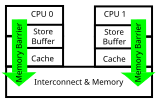
\includegraphics{memorder/SystemArchSB-smb}}
\caption{对称 Memory Barrier 交互}
\label{fig:memorder:Symmetric Memory Barriers Interactions}
\end{figure}

回顾在
\cref{sec:memorder:Rules of Thumb}
中对
\cref{fig:memorder:If-Then Nature of Memory Ordering}
的讨论（在
\cpageref{fig:memorder:If-Then Nature of Memory Ordering} 上），
给定 CPU 的 memory-barrier 指令仅与内存子系统（store buffer、cache 和互连）交互，
而不直接与其他 CPU 交互。
这意味着为了两个 CPU 彼此同步，每个 CPU 都必须执行
memory-barrier 指令，如
\cref{fig:memorder:Symmetric Memory Barriers Interactions}
中 CPU~0 和~1 所示。
考虑到 memory-barrier 配对及其推广 cycle 的需求，这并不令人惊讶。

\QuickQuiz{
	\cref{fig:memorder:Symmetric Memory Barriers Interactions}
	显示 memory barrier 与 store buffer、cache、互连和内存交互。
	但轻量级 memory-ordering 操作（load-acquire、
	store-release 和 PowerPC \co{lwsync} 指令）不是只与
	store buffer 交互吗？
}\QuickQuizAnswer{
	在很多情况下确实如此，如
	\cref{fig:memorder:Light-Weight Symmetric Memory Barriers Interactions}
	所示。

	\begin{figure}
	\centering
	\resizebox{2.5in}{!}{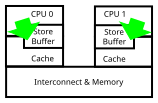
\includegraphics{memorder/SystemArchSB-slmb}}
	\caption{轻量级对称 Memory Barrier 交互}
	\label{fig:memorder:Light-Weight Symmetric Memory Barriers Interactions}
	\end{figure}

	然而，尽管这通常是正确的，但它是一种过度简化。
	轻量级 memory-ordering 操作之所以可以只与 store buffer 交互，
	唯一的原因是 cache-coherence 协议将这些交互传播到
	cache 中，cache 进而将所需的排序通过互连传播，
	如果需要的话，传播到内存。
}\QuickQuizEnd

\begin{figure}
\centering
\resizebox{2.5in}{!}{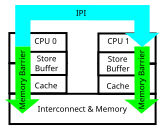
\includegraphics{memorder/SystemArchSB-amb}}
\caption{非对称 Memory Barrier 交互}
\label{fig:memorder:Asymmetric Memory Barriers Interactions}
\end{figure}

\emph{非对称 memory barrier} 背后的技巧是创建一个
\emph{重量级} memory barrier，当给定 CPU 执行它时，
不仅与内存子系统交互，还直接与目标 CPU 交互，
例如，通过向这些 CPU 发送 \IXacrfpl{ipi}。
这些目标 CPU 然后与内存子系统交互，在许多架构上，
这仅通过处理 IPI 就可以发生。
这由
\cref{fig:memorder:Asymmetric Memory Barriers Interactions}
描绘，它显示 CPU~0 执行 memory-barrier 指令但也向 CPU~1 发送 IPI。
当 CPU~1 执行 IPI 处理程序时，它也执行 memory-barrier 指令，
从而提供所需的 memory-barrier 配对，但不需要 CPU~1 自行
执行任何 memory-barrier 指令。
CPU~0 的 memory barrier 结合其 IPI（因此结合 CPU~1 的非自愿
memory barrier）构成了重量级 memory barrier。

然而，CPU~1 不能完全被动，因为编译器可以重排内存引用操作，
这可能会破坏排序。
因此 CPU~1 的代码必须包含 Linux 内核的 \co{barrier()}
编译器指令，这被称为\emph{轻量级} memory barrier。

重量级非对称 memory barrier 可以与对称 memory barrier
（或任何其他提供足够排序的操作）配对，
也可以与重量级或轻量级非对称 memory barrier 配对。
换句话说，重量级非对称 memory barrier 可以与对称
memory barrier 能配对的所有东西配对，它还可以与
轻量级非对称 memory barrier 配对。
然而，轻量级非对称 memory barrier \emph{只能}与
重量级 memory barrier 配对。
% @@@ Double-check this with litmus tests.

许多系统提供对重量级非对称 memory barrier 的用户空间访问。
例如，Linux 提供了 \co{membarrier()} 系统
调用~\cite{Corbet2010membarrier}。
但公平地说，早在 2008 年，Windows 就开始
提供 \co{FlushProcessWriteBuffers()} 系统调用。

\QuickQuiz{
	RCU 不是早在 2000 年之前就作为非对称 memory barrier 的
	一个例子吗？重量级 barrier 由 \co{synchronize_rcu()} 提供，
	轻量级 barrier 则是 \co{rcu_read_lock()} 和
	\co{rcu_read_unlock()} 之间你想要的任何地方的隐式 barrier？
}\QuickQuizAnswer{
	算是吧？

	如果你持这种观点，你可以将非对称 memory barrier
	视为针对特定 RCU 用例的优化。
	毕竟，与 \co{synchronize_rcu()} 不同，重量级非对称
	barrier 无需等待 RCU 静默状态。

	但如果你想追溯到 2008 年之前，2001 年的一个 Linux 内核
	补丁针对 DEC Alpha 上维护地址依赖的特殊情况实现了
	非对称 memory barrier~\cite{McKenney01f}。
	还有未经证实的传言称 DEC 的 Digital UNIX 在 1990 年代
	就使用了非对称 memory barrier。

	但我们可能需要面对这样一个事实：非对称 memory barrier 的
	发明已经消失在时间的沙尘中。
}\QuickQuizEnd

% @@@ Formal verification emulation in ~/paper/cpp-threads/2026/afence.
% @@@ Could add these to LKMM by encoding memory order into function name.
% @@@ Might be able to prototype them in herd7's C++ memory model?

目前，不同的环境中存在不同的非对称 barrier API，
但有一个提案建议向 C++ 标准添加特定的非对称 fence
API~\cite{DavidGoldblatt2022asymmetricFences}。

\subsection{更高层次原语：
	    讨论}
\label{sec:memorder:Higher-Level Primitives: Discussion}

用高层原语而不是该原语特定实现中使用的
低层内存访问来验证代码是非常有益的。
首先，这允许使用这些原语的代码
针对这些原语的抽象表示进行验证，
从而使该代码不太容易受到实现更改的影响。
其次，在 API 边界处划分验证会导致
组合爆炸的内爆，大大减少了形式化
验证的开销。

希望针对高层原语的详细语义进行验证
将大大提高静态分析和模型检查的有效性。

\section{硬件细节}
\label{sec:memorder:Hardware Specifics}
\OriginallyPublished{sec:memorder:Hardware Specifics}{Memory-Barrier Instructions For Specific CPUs}{Linux Journal}{PaulMcKenney2005i,PaulMcKenney2005j}
%
\epigraph{石头赢纸！}{Derek Williams}

每个CPU家族都有自己独特的memory ordering方法，
这可能使可移植性成为挑战，正如你在以下内容中看到的：
\cref{tab:memorder:Summary of Memory Ordering}.

\begin{table*}[tb] % @@@ Omitting 'p' prevents unordered floats in 2c builds
\rowcolors{4}{}{lightgray}
\small
\centering
\newcommand{\cpufml}[1]{\begin{picture}(6,50)(0,0)\rotatebox{90}{#1}\end{picture}}
\renewcommand*{\arraystretch}{1.2}\OneColumnHSpace{-.35in}
\ebresizewidth{
\begin{tabular}{llccccccccc}
	\toprule
	\multicolumn{2}{l}{~} & \multicolumn{9}{c}{CPU Family} \\
	\cmidrule{3-11}
	\multicolumn{2}{c}{\raisebox{.5ex}{Property}}
	& \cpufml{Alpha}
	& \cpufml{\ARMv7-A/R}
	& \cpufml{\ARMv8}
	& \cpufml{Itanium}
	& \cpufml{MIPS}
	& \cpufml{\Power{}}
	& \cpufml{SPARC TSO}
	& \cpufml{x86}
	& \cpufml{z~Systems}
	\\
	\cmidrule(r){1-2} \cmidrule{3-11}
%		 Alpha ARMv8 ARMv7 Itanium MIPS PPC SPARC x86 z Systems
\cellcolor{white}
	Memory Ordering
	& Loads Reordered After Loads or Stores?
		 & Y   & Y   & Y   & Y     & Y  & Y & ~   & ~ & ~ \\
	& Stores Reordered After Stores?
		 & Y   & Y   & Y   & Y     & Y  & Y & ~   & ~ & ~ \\
\cellcolor{white}
	& Stores Reordered After Loads?
		 & Y   & Y   & Y   & Y     & Y  & Y & Y   & Y & Y \\
	& \parbox[c][6ex]{2in}{\raggedright Atomic Instructions Reordered With\par Loads or Stores?}
		 & Y   & Y   & Y   & ~     & Y  & Y & ~   & ~ & ~ \\
\cellcolor{white}
	& Dependent Loads Reordered?
		 & Y   & ~   & ~   & ~     & ~  & ~ & ~   & ~ & ~ \\
	& Dependent Stores Reordered?
		 & ~   & ~   & ~   & ~     & ~  & ~ & ~   & ~ & ~ \\
\cellcolor{white}
	& Non-Sequentially Consistent?
		 & Y   & Y   & Y   & Y     & Y  & Y & Y   & Y & Y \\
	& Non-Multicopy Atomic?
		 & Y   & Y   & Y   & Y     & Y  & Y & Y   & Y & ~ \\
\cellcolor{white}
	& Non-Other-Multicopy Atomic?
		 & Y   & Y   & ~   & Y     & Y  & Y & ~   & ~ & ~ \\
	& Non-Cache Coherent?
		 & ~   & ~   & ~   & Y     & ~  & ~ & ~   & ~ & ~ \\
	\cmidrule(r){1-2} \cmidrule{3-11}
\cellcolor{white}
	Instructions
	& Load-Acquire/Store-Release?
		 & F   & F   & i   & I     & F  & b & ~   & ~ & ~ \\
	& Atomic RMW Instruction Type?
		 & L   & L   & L   & C     & L  & L & C   & C & C \\
\cellcolor{white}
	& Incoherent Instruction Cache/Pipeline?
		 & Y   & Y   & Y   & Y     & Y  & Y & Y   & Y & Y \\
	\bottomrule
\end{tabular}
}

\vspace{5pt}\hfill
\ebresizeverb{.6}{
\framebox[\width]{\footnotesize\setlength{\tabcolsep}{3pt}
\rowcolors{1}{}{}
\renewcommand*{\arraystretch}{1}
\begin{tabular}{llcl}
	{ \bf Key: }
	  & \multicolumn{3}{l}{Load-Acquire/Store-Release?} \\
	~ & ~ & b: & Lightweight memory barrier \\
	~ & ~ & F: & Full memory barrier \\
	~ & ~ & i: & Instruction with lightweight ordering \\
	~ & ~ & I: & Instruction with heavyweight ordering \\
	~ &\multicolumn{3}{l}{Atomic RMW Instruction Type?} \\
	~ & ~ & C: & Compare-and-exchange instruction \\
	~ & ~ & L: & Load-linked/store-conditional instruction \\
\end{tabular}
}
}\OneColumnHSpace{-0.4in}
\caption{Memory Ordering总结}
\label{tab:memorder:Summary of Memory Ordering}
\end{table*}

事实上，某些软件环境甚至完全禁止
直接使用memory-ordering操作，将程序员限制于
在需要的范围内包含这些操作的互斥原语。
请注意，本节并非旨在成为涵盖每个CPU家族
所有（甚至大多数）方面的参考手册，而是
提供粗略比较的高层概述。
有关完整详细信息，请参见感兴趣的CPU的参考手册。

回到
\cref{tab:memorder:Summary of Memory Ordering}，
第一组行查看内存排序属性，
第二组行查看指令属性。
请注意，这些属性在机器指令级别成立。
编译器可以并且确实比硬件更激进地重排。
使用标记的访问（如 \co{READ_ONCE()} 和 \co{WRITE_ONCE()}）
来约束编译器的优化并防止不良重排。

前三行指示给定 CPU 是否允许
加载和存储的四种可能组合被重排，如
\cref{sec:memorder:Ordering: Why and How?} 和
\crefrange{sec:memorder:Load Followed By Load}{sec:memorder:Store Followed By Store} 中所讨论的。
下一行（``原子指令与加载或存储重排？\@''）
指示给定 CPU 是否允许加载和存储
与原子指令重排。

第五和第六行涵盖重排和依赖关系，
在
\crefrange{sec:memorder:Address Dependencies}{sec:memorder:Control Dependencies} 中讨论，
并在
\cref{sec:memorder:Alpha} 中有更详细的解释。
简短的版本是 Alpha 要求链接数据结构的读者和更新者
都使用内存屏障，然而，这些内存屏障
由 v4.15 及更高版本 Linux 内核中的 Alpha 特定代码提供。

下一行，``非顺序一致性''，指示
CPU 的正常加载和存储指令是否受
顺序一致性的约束。
性能考虑决定了没有现代主流
系统是顺序一致的。

接下来三行涵盖 \IXalt{multicopy atomicity}{multi-copy atomic}，
在
\cref{sec:memorder:Multicopy Atomicity} 中定义。
第一个是完全的（且罕见的）
\IXalt{multicopy atomicity}{multi-copy atomic}，第二个是
较弱的 \IXalthy{other-multicopy atomicity}{other-}{multi-copy atomic}，
第三个是最弱的
\IXalthy{non-multicopy atomicity}{non-}{multi-copy atomic}。

下一行，``非缓存一致性''，涵盖多个
thread 对单个变量的访问，在
\cref{sec:memorder:Cache Coherence} 中讨论。

最后三行涵盖指令级别的选择和问题。
第一行指示每个 CPU 如何实现 load-acquire
和 store-release，第二行按原子指令类型对 CPU 进行分类，
第三行即最后一行
指示给定 CPU 是否具有不一致的
指令缓存和流水线。
这类 CPU 需要为自修改代码执行特殊指令。

%Parenthesized CPU names indicate modes that are architecturally allowed,
%but rarely used in practice.

常见的``直接拒绝''内存排序操作方法
在适用的地方是完全合理的，
但在某些环境中（如 Linux 内核），需要直接
使用内存排序操作。
因此，
Linux 提供了一组精心选择的最小公分母
内存排序原语，如下所示：
\begin{description}
\item	[\tco{smp_mb()}] (\IXh{full}{memory barrier}) that orders both loads and
	stores.
	This means that loads and stores preceding the memory barrier
	will be committed to memory before any loads and stores
	following the memory barrier.
\item	[\tco{smp_rmb()}] (\IXh{read}{memory barrier}) that orders only loads.
\item	[\tco{smp_wmb()}] (\IXh{write}{memory barrier}) that orders only stores.
\item	[\tco{smp_mb__before_atomic()}] that forces ordering of accesses
	preceding the \co{smp_mb__before_atomic()} against accesses following
	a later RMW atomic operation.
	This is a noop on systems that fully order atomic RMW operations.
\item	[\tco{smp_mb__after_atomic()}] that forces ordering of accesses
	preceding an earlier RMW atomic operation against accesses
	following the \co{smp_mb__after_atomic()}.
	This is also a noop on systems that fully order atomic RMW operations.
\item	[\tco{smp_mb__after_spinlock()}] that forces ordering of accesses
	preceding a lock acquisition against accesses
	following the \co{smp_mb__after_spinlock()}.
	This is also a noop on systems that fully order lock acquisitions.
\item	[\tco{mmiowb()}] that forces ordering on MMIO writes that are guarded
	by global spinlocks, and is more thoroughly described
	in a 2016 LWN article on MMIO~\cite{PaulEMcKenney2016LinuxKernelMMIO}.
\end{description}
The \co{smp_mb()}、\co{smp_rmb()} 和 \co{smp_wmb()}
原语还强制编译器避免任何会导致
跨屏障重排内存优化的优化。

\QuickQuiz{
	原子操作和
	\co{smp_mb__after_atomic()} 之间的代码会怎样？
}\QuickQuizAnswer{
	首先，请不要这样做！

	但如果你这样做，这段中间代码要么被排在
	原子操作之后，要么被排在
	\co{smp_mb__after_atomic()} 之前，取决于架构，
	但不能同时满足两者。
	这也适用于 \co{smp_mb__before_atomic()} 和
	\co{smp_mb__after_spinlock()}，即中间代码不确定的
	排序以及避免此类代码的请求。
}\QuickQuizEnd

这些原语仅在 SMP 内核中生成代码，但有几个
具有 UP 版本（分别是 \co{mb()}、\co{rmb()} 和 \co{wmb()}），
即使在 UP 内核中也会生成内存屏障。
在大多数情况下应使用 \co{smp_} 版本。
然而，后者在编写驱动程序时很有用，
因为即使在 UP 内核中，MMIO 访问也必须保持有序。
在没有内存排序操作的情况下，CPU 和编译器
都会愉快地重新排列这些访问，
这最好会使设备表现异常，
并可能使内核崩溃甚至损坏硬件。

因此，大多数内核程序员不必担心每个 CPU 的
内存排序特性，只要他们坚持使用这些
接口和完全有序的原子操作即可。\footnote{
	For a full list, expand the patterns in
	\path{Documentation/atomic_t.txt}.}
当然，如果你在给定 CPU 的特定于架构的代码中深入工作，
一切都不可预料。

此外，
Linux 的所有锁原语（自旋锁、读写锁、
信号量、RCU、\ldots）都包含任何需要的排序原语。
因此，如果你使用的代码正确使用了这些原语，
你就不必担心 Linux 的内存排序原语。

话虽如此，深入了解每个 CPU 的
\IXalt{memory-consistency model}{memory model}
在调试时非常有帮助，更不用说在编写
特定于架构的代码或同步原语时了。

此外，俗话说一知半解是非常危险的事情。
想想你拥有大量知识可能造成的损害！
对于那些希望了解更多关于各个 CPU
内存一致性模型的人，接下来的几节描述了一些
流行和重要 CPU 的模型。
虽然没有什么可以替代真正阅读给定 CPU 的
文档，但这些章节确实提供了很好的概述。

\subsection{Alpha}
\label{sec:memorder:Alpha}

谈论一个早已停产的 CPU 似乎有些奇怪，但 Alpha 很有趣，
因为它是唯一一个重排依赖加载的主流 CPU，因此对并发 API（包括
Linux 内核中的 API）产生了巨大影响。
Linux 内核核心代码需要适配 Alpha 的需求
随着 Linux 内核 v4.15 版本而结束，这种适配的所有痕迹
在 v5.9 中随着 \apikh{smp_read_barrier_depends()} 和
\co{read_barrier_depends()} API 的移除而被移除。
本节在第三版中仍然保留，
因为到 2023 年初，仍有一些 Linux 内核黑客
仍在使用 v4.15 之前的 Linux 内核版本。
此外，允许移除这些 API 的 \co{READ_ONCE()} 修改
可能尚未传播到所有可能仍支持 Alpha 的
用户空间项目。

\begin{fcvref}[ln:memorder:Insert and Lock-Free Search (No Ordering)]
Alpha 与其他 CPU 之间的依赖加载差异
由
\cref{lst:memorder:Insert and Lock-Free Search (No Ordering)} 中显示的代码说明。
此 \co{smp_store_release()}
保证 \clnrefrange{init:b}{init:e} 中的元素初始化
在元素通过 \clnref{add} 添加到列表之前执行，
因此无锁搜索将正确工作。
也就是说，它在除 Alpha 之外的所有 CPU 上都做出此保证。
\end{fcvref}

\begin{listing}
\begin{fcvlabel}[ln:memorder:Insert and Lock-Free Search (No Ordering)]
\begin{VerbatimL}[commandchars=\\\[\]]
struct el *insert(long key, long data)
{
	struct el *p;
	p = kmalloc(sizeof(*p), GFP_ATOMIC);
	spin_lock(&mutex);
	p->next = head.next;		\lnlbl[init:b]
	p->key = key;
	p->data = data;			\lnlbl[init:e]
	smp_store_release(&head.next, p); \lnlbl[add]
	spin_unlock(&mutex);
}

struct el *search(long searchkey)
{
	struct el *p;
	p = READ_ONCE_OLD(head.next);	\lnlbl[h:next]
	while (p != &head) {
		/* Prior to v4.15, BUG ON ALPHA!!! */ \lnlbl[BUG]
		if (p->key == searchkey) {	\lnlbl[key]
			return (p);
		}
		p = READ_ONCE_OLD(p->next);	\lnlbl[next]
	};
	return (NULL);
}
\end{VerbatimL}
\end{fcvlabel}
\caption{插入和无锁搜索（无排序）}
\label{lst:memorder:Insert and Lock-Free Search (No Ordering)}
\end{listing}

\begin{fcvref}[ln:memorder:Insert and Lock-Free Search (No Ordering)]
鉴于 \co{READ_ONCE_OLD()} 表示的 v4.15 之前 \co{READ_ONCE()} 的实现，
Alpha 实际上允许
\cref{lst:memorder:Insert and Lock-Free Search (No Ordering)}
中 \clnref{key} 处的代码
看到 \clnrefrange{init:b}{init:e} 初始化之前存在的旧垃圾值。

\Cref{fig:memorder:fig:memorder:Why smp-read-barrier-depends() is Required in Pre-v4.15 Linux Kernels}
展示了这如何在具有分区缓存的
积极并行机器上发生，使得交替的 \IXpl{cache line}
由缓存的不同分区处理。
例如，\cref{lst:memorder:Insert and Lock-Free Search (No Ordering)}
中 \clnref{h:next} 处对 \co{head.next} 的加载
可能访问缓存 bank~0，
\clnref{key} 处对 \co{p->key} 和 \clnref{next} 处对 \co{p->next} 的加载
可能访问缓存 bank~1。
在 Alpha 上，\co{smp_store_release()} 将保证
\cref{lst:memorder:Insert and Lock-Free Search (No Ordering)}
中 \clnrefrange{init:b}{init:e} 执行的缓存失效
（针对 \co{p->next}、\co{p->key} 和 \co{p->data}）
将在 \clnref{add}（针对 \co{head.next}）的缓存失效
之前到达互连，但对通过读取 CPU 的缓存 bank 的
传播顺序不提供任何保证。
例如，读取 CPU 的缓存 bank~1 可能非常繁忙，
但缓存 bank~0 空闲。
这可能导致新元素（\co{p->next}、\co{p->key} 和 \co{p->data}）的
缓存失效被延迟，
使得读取 CPU 加载 \co{head.next} 的新值，
但加载 \co{p->key} 和 \co{p->next} 的旧缓存值。
是的，这确实意味着 Alpha 实际上可以在
获取指针本身之前获取指针指向的数据，奇怪
但确实如此。
\end{fcvref}
更多信息请参见前面提到的文档~\cite{Compaq01,WilliamPugh2000Gharachorloo}，
或者你认为我只是在编造这一切的话。\footnote{
	当然，敏锐的读者已经认识到
	Alpha 远没有它可能的那样恶劣，
	\cref{sec:app:whymb:Ordering-Hostile Architecture}
	中（谢天谢地是虚构的）架构就是一个很好的例子。}
这种不寻常的排序方法的好处是 Alpha 可以使用
更简单的缓存硬件，这反过来在 Alpha 的鼎盛时期
允许了更高的时钟频率。

\begin{figure}
\centering
\resizebox{\twocolumnwidth}{!}{\includegraphics{memorder/Alpha}}
\caption{为什么Pre-v4.15 Linux内核需要\tco{smp_read_barrier_depends()}}
\label{fig:memorder:fig:memorder:Why smp-read-barrier-depends() is Required in Pre-v4.15 Linux Kernels}
\end{figure}

可以在指针获取和解引用之间放置 \co{smp_rmb()} 原语
以强制 Alpha 将指针获取与后续依赖加载排序。
然而，这会在读取侧尊重
\IXalth{address dependencies}{address}{dependency} 的系统
（如 \ARM、Itanium、PPC 和 SPARC）上强加不必要的开销。
因此，在 Linux 内核中添加了 \co{smp_read_barrier_depends()} 原语
以消除这些系统上的开销，但在 Linux 内核 v5.9 中被移除，
取而代之的是增强 Alpha 对 \co{READ_ONCE()} 的定义。
因此，从 v5.9 开始，核心内核代码不再需要关心
DEC Alpha 的这一方面。
\begin{fcvref}[ln:memorder:Safe Insert and Lock-Free Search]
然而，最好使用 \co{rcu_dereference()}，
如
\cref{lst:memorder:Safe Insert and Lock-Free Search} 中 \clnref{deref1,deref2} 所示，
它对所有最近的内核版本都能安全高效地工作。
\end{fcvref}

也可以实现一种软件机制，
用于替代 \co{smp_store_release()} 以强制
所有读取 CPU 按顺序看到写入 CPU 的写入。
这种软件屏障可以通过向所有其他 CPU 发送 \IXacrfpl{ipi}
来实现。
收到这样的 IPI 时，CPU 将执行内存屏障指令，
实现类似 Linux 内核 \co{sys_membarrier()} 系统调用提供的
系统级内存屏障，因此是
\cref{sec:memorder:Asymmetric Memory Barriers} 中讨论的
非对称内存屏障的早期示例。
需要额外的逻辑来避免死锁。
当然，尊重地址依赖的 CPU 会将这样的屏障
简单地定义为 \co{smp_store_release()}。
然而，这种方法被 Linux 社区认为
会施加过多的开销~\cite{McKenney01f}，而且对于具有
激进实时响应要求的系统来说完全不合适。

\begin{listing}
\begin{fcvlabel}[ln:memorder:Safe Insert and Lock-Free Search]
\begin{VerbatimL}[commandchars=\\\[\]]
struct el *insert(long key, long data)
{
	struct el *p;
	p = kmalloc(sizeof(*p), GFP_ATOMIC);
	spin_lock(&mutex);
	p->next = head.next;
	p->key = key;
	p->data = data;
	smp_store_release(&head.next, p);
	spin_unlock(&mutex);
}

struct el *search(long searchkey)
{
	struct el *p;
	p = rcu_dereference(head.next);		\lnlbl[deref1]
	while (p != &head) {
		if (p->key == searchkey) {
			return (p);
		}
		p = rcu_dereference(p->next);	\lnlbl[deref2]
	};
	return (NULL);
}
\end{VerbatimL}
\end{fcvlabel}
\caption{安全的插入和无锁搜索}
\label{lst:memorder:Safe Insert and Lock-Free Search}
\end{listing}

Linux 内存屏障原语的名称取自 Alpha
指令，因此 \co{smp_mb()} 是 \co{mb}，\co{smp_rmb()} 是 \co{rmb}，
\co{smp_wmb()} 是 \co{wmb}。
Alpha 是唯一一个 \co{READ_ONCE()} 包含 \co{smp_mb()} 的 CPU。

\QuickQuizSeries{%
\QuickQuizB{
	Why does Alpha's \co{READ_ONCE()} include an
	\co{mb()} rather than \co{rmb()}?
}\QuickQuizAnswerB{
	Alpha has only \co{mb} and \co{wmb} instructions,
	so \co{smp_rmb()} would be implemented by the Alpha \co{mb}
	instruction in either case.
	In addition, at the time that the Linux kernel started relying on
	dependency ordering, it was not clear that Alpha ordered dependent
	stores, and thus \co{smp_mb()} was therefore the safe choice.

	However, given the aforementioned v5.9 changes to \co{READ_ONCE()}
	and a few of Alpha's atomic read-modify-write operations,
	no Linux-kernel core code need concern itself with DEC Alpha,
	thus greatly reducing Paul E.~McKenney's incentive to remove
	Alpha support from the kernel.
}\QuickQuizEndB
%
\QuickQuizE{
	Isn't DEC Alpha significant as having the weakest possible
	memory ordering?
}\QuickQuizAnswerE{
	Although DEC Alpha does take considerable flak, it does avoid
	reordering reads from the same CPU to the same variable.
	It also avoids the out-of-thin-air problem that plagues
	the Java and C11 memory
	models~\cite{Boehm:2014:OGA:2618128.2618134,conf/esop/BattyMNPS15,MarkBatty2013OOTA-WorkingNote,HansBoehm2020ConcurrentUB,DavidGoldblatt2019NoElegantOOTAfix,AlanJeffrey2014JavaDRF,PaulEMcKenney2020RelaxedGuideRelaxed,PaulEMcKenney2016OOTA,Sevcik:2011:SOS:1993316.1993534,Vafeiadis:2015:CCO:2775051.2676995}.
}\QuickQuizEndE
}

关于 Alpha 的更多信息，请参见其参考手册~\cite{ALPHA2002}。

\subsection{\ARMv7-A/R}
\label{sec:memorder:ARMv7-A/R}

\ARM\ CPU 系列在深度嵌入式应用中很流行，
特别是对于功耗受限的微控制器。
其 \IXalthmr{memory model}{Armv7}{memory model} 类似于 \Power{}
（参见 \cref{sec:memorder:POWER / PowerPC}），但 \ARM\ 使用
不同的内存屏障指令集~\cite{ARMv7A:2010}：

\begin{description}
\item	[\tco{DMB}] (data memory barrier) causes the specified type of
	operations to \emph{appear} to have completed before any
	subsequent operations of the same type.
	The ``type'' of operations can be all operations or can be
	restricted to only writes (similar to the Alpha \co{wmb}
	and the \Power{} \co{eieio} instructions).
	In addition, \ARM\ allows \IX{cache coherence} to have one of three
	scopes:
	Single processor, a subset of the processors
	(``inner'') and global (``outer'').
\item	[\tco{DSB}] (data synchronization barrier) causes the specified
	type of operations to actually complete before any subsequent
	operations (of any type) are executed.
	The ``type'' of operations is the same as that of \co{DMB}.
	The \co{DSB} instruction was called \co{DWB} (drain write buffer
	or data write barrier, your choice) in early versions of the
	\ARM\ architecture.
\item	[\tco{ISB}] (instruction synchronization barrier) flushes the CPU
	pipeline, so that all instructions following the \co{ISB}
	are fetched only after the \co{ISB} completes.
	For example, if you are writing a self-modifying program
	(such as a JIT), you should execute an \co{ISB} between
	generating the code and executing it.
\end{description}

这些指令中没有一个完全匹配 Linux 的
\co{rmb()} 原语的语义，因此必须作为完整的
\co{DMB} 实现。
\co{DMB} 和 \co{DSB} 指令对屏障前后排序的访问
具有递归定义，其效果类似于 \Power{} 的累积性，
两者都比
\cref{sec:memorder:Cumulativity} 中描述的
\IXalthmr{\acr{lkmm}}{Linux kernel}{memory model} 的累积性更强。

\ARM\ also implements \IXalth{control dependencies}{control}{dependency},
so that if a conditional
branch depends on a load, then any store executed after that conditional
branch will be ordered after the load.
然而，条件分支之后的加载 \emph{不会}保证被排序，
除非分支和加载之间有 \co{ISB}
指令。
考虑以下示例：

\begin{fcvlabel}[ln:memorder:ARM:load-store control dependency]
\begin{VerbatimN}[commandchars=\\\[\]]
r1 = x;			\lnlbl[x]
if (r1 == 0)		\lnlbl[if]
	nop();		\lnlbl[nop]
y = 1;			\lnlbl[y]
r2 = z;			\lnlbl[z1]
ISB();			\lnlbl[isb]
r3 = z;			\lnlbl[z2]
\end{VerbatimN}
\end{fcvlabel}

\begin{fcvref}[ln:memorder:ARM:load-store control dependency]
在此示例中，加载-存储控制依赖排序导致
\clnref{x} 处对 \co{x} 的加载被排在
\clnref{y} 处对 \co{y} 的存储之前。
然而，\ARM\ 不尊重加载-加载控制依赖，因此
\clnref{x} 处的加载很可能发生在
\clnref{z1} 处的加载 \emph{之后}。
另一方面，\clnref{if} 处的条件分支和
\clnref{isb} 处的 \co{ISB} 指令的组合确保
\clnref{z2} 处的加载发生在 \clnref{x} 处的加载之后。
注意，在 \clnref{if,z1} 之间的某处插入额外的 \co{ISB} 指令
将强制 \clnref{x,z1} 之间的排序。
\end{fcvref}

\subsection{\ARMv8}
\label{sec:memorder:ARMv8}

\begin{figure}
\centering
\resizebox{2in}{!}{\includegraphics{cartoons/r-2014-LDLAR}}
\caption{半Memory Barrier}
\ContributedBy{fig:memorder:Half Memory Barrier}{Melissa Brossard}
\end{figure}

\ARM's \ARMv8 CPU family~\cite{ARMv8A:2017}
includes 64-bit capabilities,
in contrast to their 32-bit-only CPU described in
\cref{sec:memorder:ARMv7-A/R}.
\IXalthmr{\ARMv8's memory model}{Armv8}{memory model}
closely resembles its \ARMv7 counterpart,
but adds load-acquire (\co{LDLARB}, \co{LDLARH}, and \co{LDLAR})
and store-release (\co{STLLRB}, \co{STLLRH}, and \co{STLLR})
instructions.
这些指令充当``半内存屏障''，因此
\ARMv8 CPU 可以将先前的访问与后续的 \co{LDLAR}
指令重排，但不允许将较早的 \co{LDLAR}
指令与后续访问重排，如
\cref{fig:memorder:Half Memory Barrier} 所示。
类似地，\ARMv8 CPU 可以将较早的 \co{STLLR} 指令与
后续访问重排，但不允许将
先前的访问与后续的 \co{STLLR} 指令重排。
正如人们可能期望的，这意味着这些指令直接支持
C11 的 load-acquire 和 store-release 概念。

然而，\ARMv8 通过要求在某些情况下
store-release 和 load-acquire 的组合作为完全屏障
而远远超越了 C11 内存模型。
例如，在 \ARMv8 中，给定一个存储后跟一个 store-release，再后跟
一个 load-acquire，再后跟一个加载，所有操作针对不同的变量且都来自
单个 CPU，所有 CPU
都将同意初始存储先于最终加载。
有趣的是，大多数 TSO 架构（包括 x86 和
大型机）不做这个保证，因为两个加载可以
在两个存储之前被重排。

\ARMv8 是仅有的两个需要
\co{smp_mb__after_spinlock()} 原语作为完全屏障的架构之一，
这是由于其在 Linux 内核中
相对较弱的锁获取实现。

\ARMv8 还具有成为第一个由其供应商公开
使用可执行形式模型定义其内存排序的 CPU 的殊荣~\cite{ARMv8A:2017}。

\subsection{Itanium}
\label{sec:memorder:Itanium}

Itanium 提供 \IXalth{weak consistency}{weak}{memory consistency}
\IXalthmr{model}{Itanium}{memory model}，因此在没有显式
内存屏障指令或依赖关系的情况下，Itanium 有权
任意重排内存引用~\cite{IntelItanium02v2}。
Itanium 有一个名为 \co{mf} 的内存围栏指令，但还有
``半内存围栏''修饰符用于加载、存储和一些原子
指令~\cite{IntelItanium02v3}。
\co{acq} 修饰符阻止后续内存引用指令
在 \co{acq} 之前被重排，但允许
先前的内存引用指令在 \co{acq} 之后被重排，
类似于 \ARMv8 的 load-acquire 指令。
类似地，\co{rel} 修饰符阻止先前的内存引用
指令在 \co{rel} 之后被重排，但允许
后续内存引用指令在 \co{rel} 之前被重排。

这些半内存围栏对临界区很有用，因为
将操作推入临界区是安全的，但允许它们
泄漏出去可能是致命的。
然而，作为少数具有此属性的 CPU 之一，Itanium 曾经
定义了 Linux 与锁获取和释放相关的内存排序语义。\footnote{
	PowerPC 现在是拥有这一可疑特权的架构。}
奇怪的是，据传实际的 Itanium 硬件将
load-acquire 和 store-release 指令都实现为完全屏障。
尽管如此，Itanium 是第一个将 load-acquire 和 store-release 的概念
（如果不是现实的话）引入其指令集的主流 CPU。

\QuickQuiz{
	Given that hardware can have a half memory barrier, why don't
	locking primitives allow the compiler to move memory-reference
	instructions into lock-based critical sections?
}\QuickQuizAnswer{
	In fact, as we saw in \cref{sec:memorder:ARMv8} and will
	see in \cref{sec:memorder:POWER / PowerPC}, hardware really does
	implement partial memory-ordering instructions and it also turns
	out that these really are used to construct locking primitives.
	However, these locking primitives use full compiler barriers,
	thus preventing the compiler from reordering memory-reference
	instructions both out of and into the corresponding critical
	section.

\begin{listing}
\begin{fcvlabel}[ln:memorder:synchronize-rcu]
\begin{VerbatimL}[commandchars=\@\[\]]
static inline int rcu_gp_ongoing(unsigned long *ctr)
{
	unsigned long v;

	v = LOAD_SHARED(*ctr);@lnlbl[load]
	return v && (v != rcu_gp_ctr);
}

static void update_counter_and_wait(void)
{
	struct rcu_reader *index;

	STORE_SHARED(rcu_gp_ctr, rcu_gp_ctr + RCU_GP_CTR);
	barrier();
	list_for_each_entry(index, &registry, node) {@lnlbl[loop]
		while (rcu_gp_ongoing(&index->ctr))@lnlbl[call2]
			msleep(10);
	}
}

void synchronize_rcu(void)
{
	unsigned long was_online;

	was_online = rcu_reader.ctr;
	smp_mb();
	if (was_online)@lnlbl[if]
		STORE_SHARED(rcu_reader.ctr, 0);@lnlbl[store]
	mutex_lock(&rcu_gp_lock);@lnlbl[acqmutex]
	update_counter_and_wait();@lnlbl[call1]
	mutex_unlock(&rcu_gp_lock);
	if (was_online)
		STORE_SHARED(rcu_reader.ctr, LOAD_SHARED(rcu_gp_ctr));
	smp_mb();
}
\end{VerbatimL}
\end{fcvlabel}
\caption{用户空间RCU代码重排}
\label{lst:memorder:Userspace RCU Code Reordering}
\end{listing}

	To see why the compiler is forbidden from doing reordering that
	is permitted by hardware, consider the following sample code
	in \cref{lst:memorder:Userspace RCU Code Reordering}.
	This code is based on the userspace RCU update-side
	code~\cite[Supplementary Materials Figure 5]{MathieuDesnoyers2012URCU}.

\begin{fcvref}[ln:memorder:synchronize-rcu]
	Suppose that the compiler reordered \clnref{if,store} into
	the critical section starting at \clnref{acqmutex}.
	Now suppose that two updaters start executing \co{synchronize_rcu()}
	at about the same time.
	Then consider the following sequence of events:
	\begin{enumerate}
	\item	CPU~0 acquires the lock at \clnref{acqmutex}.
	\item	\Clnref{if} determines that CPU~0 was online, so it clears
		its own counter at \clnref{store}.
		(Recall that \clnref{if,store} have been reordered by the
		compiler to follow \clnref{acqmutex}).
	\item	CPU~0 invokes \co{update_counter_and_wait()} from
		\clnref{call1}.
	\item	CPU~0 invokes \co{rcu_gp_ongoing()} on itself at
		\clnref{call2}, and \clnref{load} sees that CPU~0 is
		in a quiescent state.
		Control therefore returns to \co{update_counter_and_wait()},
		and \clnref{loop} advances to CPU~1.
	\item	CPU~1 invokes \co{synchronize_rcu()}, but because CPU~0
		already holds the lock, CPU~1 blocks waiting for this
		lock to become available.
		Because the compiler reordered \clnref{if,store} to follow
		\clnref{acqmutex}, CPU~1 does not clear its own counter,
		despite having been online.
	\item	CPU~0 invokes \co{rcu_gp_ongoing()} on CPU~1 at
		\clnref{call2}, and \clnref{load} sees that CPU~1 is
		not in a quiescent state.
		The \co{while} loop at \clnref{call2} therefore never
		exits.
	\end{enumerate}

	So the compiler's reordering results in a deadlock.
	In contrast, hardware reordering is temporary, so that CPU~1
	might undertake its first attempt to acquire the mutex on
	\clnref{acqmutex} before executing \clnref{if,store}, but it
	will eventually execute \clnref{if,store}.
	Because hardware reordering only results in a short delay, it
	can be tolerated.
	On the other hand, because compiler reordering results in a
	deadlock, it must be prohibited.

	Some research efforts have used hardware transactional memory
	to allow compilers to safely reorder more aggressively, but
	the overhead of hardware transactions has thus far made
	such optimizations unattractive.
	% @@@ Citation for compilers use of HTM in this manner?
\end{fcvref}
}\QuickQuizEnd

Itanium 的 \co{mf} 指令用于 Linux 内核中的 \co{smp_rmb()}、
\co{smp_mb()} 和 \co{smp_wmb()} 原语。
尽管有持续的相反传言，\qco{mf} 助记符代表
``内存围栏''。

Itanium 还为释放操作提供全局总序，
包括 \co{mf} 指令。
这提供了传递性的概念，即如果给定代码片段
看到某个访问已经发生，任何后续代码片段
也会看到该先前访问已经发生。
也就是说，假设所有涉及的代码片段都正确使用了
内存屏障。

最后，Itanium 是支持 Linux 内核的唯一一个
可以对同一变量的正常加载进行重排的架构。
Linux 内核避免了这个问题，因为 \co{READ_ONCE()} 发出
一个 \co{volatile} 加载，它被编译为 \co{ld,acq} 指令，
这强制给定 CPU 的所有 \co{READ_ONCE()} 调用的排序，
包括对同一变量的调用。

\subsection{MIPS}

\IXhmr{MIPS}{memory model}~\cite[page~479]{MIPSvII-A-2016}
似乎类似于 \ARM、Itanium 和 \Power{}，
默认弱排序但尊重依赖关系。
MIPS 有多种内存屏障指令，但将它们
不是与硬件考虑联系起来，而是与 Linux 内核
和 C++11 标准~\cite{RichardSmith2019N4800} 提供的
用例联系起来，类似于 \ARMv8 的添加：

\begin{description}[style=nextline]
\item[\tco{SYNC}]
	Full barrier for a number of hardware operations in addition
	to memory references, which is used to implement the v4.13
	Linux kernel's \co{smp_mb()} for OCTEON systems.
\item[\tco{SYNC_WMB}]
	Write memory barrier, which can be used on OCTEON systems
	to implement the
	\co{smp_wmb()} primitive in the v4.13 Linux kernel via the
	\co{syncw} mnemonic.
	Other systems use plain \co{sync}.
\item[\tco{SYNC_MB}]
	Full memory barrier, but only for memory operations.
	This may be used to implement the
	C++ \co{atomic_thread_fence(memory_order_seq_cst)}.
\item[\tco{SYNC_ACQUIRE}]
	Acquire memory barrier, which could be used to implement
	C++'s \co{atomic_thread_fence(memory_order_acquire)}.
	In theory, it could also be used to implement the v4.13 Linux-kernel
	\co{smp_load_acquire()} primitive, but in practice
	\co{sync} is used instead.
\item[\tco{SYNC_RELEASE}]
	Release memory barrier, which may be used to implement
	C++'s \co{atomic_thread_fence(memory_order_release)}.
	In theory, it could also be used to implement the v4.13 Linux-kernel
	\co{smp_store_release()} primitive, but in practice
	\co{sync} is used instead.
\item[\tco{SYNC_RMB}]
	Read memory barrier, which could in theory be used to implement the
	\co{smp_rmb()} primitive in the Linux kernel, except that current
	MIPS implementations supported by the v4.13 Linux kernel do not
	need an explicit instruction to force ordering.
	Therefore, \co{smp_rmb()} instead simply constrains the compiler.
\item[\tco{SYNCI}]
	Instruction-cache synchronization, which is used in conjunction with
	other instructions to allow self-modifying code, such as that produced
	by just-in-time (JIT) compilers.
\end{description}

与 MIPS 架构师的非正式讨论表明，MIPS 具有类似于
\ARM\ 和 \Power{} 的传递性或累积性定义。
然而，不同的 MIPS 实现可能具有
不同的内存排序属性，因此查阅
你正在使用的特定 MIPS 实现的文档非常重要。

\subsection{\Power{} / PowerPC}
\label{sec:memorder:POWER / PowerPC}

\Power{} 和 PowerPC CPU 系列有多种内存屏障
指令~\cite{PowerPC94,MichaelLyons05a}：
\begin{description}
\item	[\tco{sync}] causes all preceding operations to {\em appear to have}
	completed before any subsequent operations are started.
	This instruction is therefore quite expensive.
\item	[\tco{lwsync}] (lightweight sync) orders loads with respect to
	subsequent loads and stores, and also orders stores.
	However, it does {\em not} order stores with respect to subsequent
	loads.
	The \co{lwsync} instruction may be used to implement
	load-acquire and store-release operations.
	Interestingly enough, the \co{lwsync} instruction enforces
	the same within-CPU ordering as does x86, z~Systems, and coincidentally,
	SPARC TSO\@.
	However, placing the \co{lwsync} instruction between each
	pair of memory-reference instructions will \emph{not}
	result in x86, z~Systems, or SPARC TSO memory ordering.
	On these other systems, if a pair of CPUs independently execute
	stores to different variables, all other CPUs will agree on the
	order of these stores.
	Not so on PowerPC, even with an \co{lwsync} instruction between each
	pair of memory-reference instructions, because PowerPC is
	\IXalthy{non-multicopy atomic}{non-}{multi-copy atomic}.
\item	[\tco{eieio}] (enforce in-order execution of I/O, in case you
	were wondering) causes all preceding cacheable stores to appear
	to have completed before all subsequent stores.
	However, stores to cacheable memory are ordered separately from
	stores to non-cacheable memory, which means that \co{eieio}
	will not force an MMIO store to precede a spinlock release.
	This instruction may well be unique in having a five-vowel mnemonic.
\item	[\tco{isync}] forces all preceding instructions to appear to have
	completed before any subsequent instructions start execution.
	This means that the preceding instructions must have progressed
	far enough that any traps they might generate have either happened
	or are guaranteed not to happen, and that any side-effects of
	these instructions (for example, page-table changes) are seen by the
	subsequent instructions.
	However, it does \emph{not} force all memory references to be
	ordered, only the actual execution of the instruction itself.
	Thus, the loads might return old still-cached values and the
	\co{isync} instruction does not force values previously stored
	to be flushed from the store buffers.
\end{description}

不幸的是，这些指令中没有一个与 Linux 的
\co{wmb()} 原语完全对齐，后者要求\emph{所有}存储被排序，
但不需要 \co{sync} 指令的其他高开销操作。
\co{rmb()} 原语也没有匹配的轻量级指令。
但别无选择：
{ppc64} 版本的 \co{wmb()}、\co{rmb()} 和 \co{mb()} 被定义为
重量级的 \co{sync} 指令。
然而，Linux 的 \co{smp_wmb()} 原语从不用于 MMIO
（毕竟驱动程序必须在 UP 和 SMP 内核中仔细排序 MMIO），
因此它被定义为更轻量级的
\co{eieio} 或 \co{lwsync} 指令~\cite{PaulEMcKenney2016LinuxKernelMMIO}。
\co{smp_mb()} 原语也被定义为 \co{sync}
指令，而 \co{smp_rmb()} 被定义为更轻量级的
\co{lwsync} 指令。

\Power{} 具有``累积性''，可用于获得传递性。
如果使用得当，任何看到较早代码片段
结果的代码也将看到该较早代码片段
本身看到的访问。
更多信息可从
McKenney 和 Silvera~\cite{PaulEMcKenneyN2745r2009} 获得。

\Power{} 以与 \ARM\ 基本相同的方式尊重控制依赖，
例外是 \Power{} 的 \co{isync} 指令
替代了 \ARM\ 的 \co{ISB} 指令。

与 \ARMv8 一样，\Power{} 要求 \co{smp_mb__after_spinlock()} 作为
完全内存屏障。
此外，\Power{} 是唯一要求
\co{smp_mb__after_unlock_lock()} 作为完全内存屏障的架构。
在这两种情况下，这是因为 \Power{} 锁原语的弱排序属性，
由于使用 \co{lwsync} 指令为获取和释放都提供排序。

\Power{} 架构的许多成员具有不一致的指令
缓存，因此对内存的存储不一定会反映在指令缓存中。
值得庆幸的是，现在很少有人编写自修改代码，但 JIT
和编译器一直在这样做。
此外，从 CPU 的角度来看，重新编译最近运行的程序
看起来就像自修改代码。
\co{icbi} 指令（指令缓存块无效化）从
指令缓存中使指定的缓存行无效化，
可在这些情况下使用。

\subsection{SPARC TSO}

虽然 SPARC 的 TSO（总存储顺序）被 Linux 和
Solaris 使用，但该架构还定义了 PSO（部分存储顺序）和 RMO
（宽松内存顺序）。
任何在 RMO 中运行的程序也将在 PSO 或 TSO 中运行，类似地，
任何在 PSO 中运行的程序也将在 TSO 中运行。
向相反方向移动共享内存并行程序可能需要
仔细插入内存屏障。

虽然 SPARC 的 PSO 和 RMO 模式现在不常使用，但它们
确实催生了一个非常灵活的内存屏障指令~\cite{SPARC94}，
允许对排序进行细粒度控制：
\begin{description}
\item	[\tco{StoreStore}] orders preceding stores before subsequent stores.
	(This option is used by the Linux \co{smp_wmb()} primitive.)
\item	[\tco{LoadStore}] orders preceding loads before subsequent stores.
\item	[\tco{StoreLoad}] orders preceding stores before subsequent loads.
\item	[\tco{LoadLoad}] orders preceding loads before subsequent loads.
	(This option is used by the Linux \co{smp_rmb()} primitive.)
\item	[\tco{Sync}] fully completes all preceding operations before starting
	any subsequent operations.
\item	[\tco{MemIssue}] completes preceding memory operations before subsequent
	memory operations, important for some instances of memory-mapped
	I/O.
\item	[\tco{Lookaside}] does the same as MemIssue,
	but only applies to preceding stores
	and subsequent loads, and even then only for stores and loads that
	access the same memory location.
\end{description}

那么，为什么需要 \qco{membar #MemIssue}？
因为 \qco{membar #StoreLoad} 可能允许后续
加载从 store buffer 获取其值，如果写入的是
对要读取的值产生副作用的 MMIO 寄存器，这将是灾难性的。
相比之下，\qco{membar #MemIssue} 将等到 store buffer
被刷新后才允许加载执行，
从而确保加载实际上从 MMIO 寄存器获取其值。
驱动程序可以改用 \qco{membar #Sync}，但在不需要
更昂贵的 \qco{membar #Sync} 的额外功能的情况下，
更倾向于使用更轻量级的 \qco{membar #MemIssue}。

\qco{membar #Lookaside} 是 \qco{membar #MemIssue} 的更轻量级版本，
当写入给定 MMIO 寄存器会影响将从该寄存器读取的下一个值时很有用。
但是，当写入给定 MMIO 寄存器会影响将从{\em 某个其他} MMIO 寄存器
读取的下一个值时，必须使用更重量级的 \qco{membar #MemIssue}。

SPARC 要求在指令流被修改和这些指令被执行之间
使用 \co{flush} 指令~\cite{SPARC94}。
这是为了从 SPARC 的指令缓存中刷新该位置的任何先前值。
注意 \co{flush} 接受一个地址，只会从指令缓存中
刷新该地址。
在 SMP 系统上，所有 CPU 的缓存都会被刷新，但没有
方便的方法来确定何时 CPU 外的刷新完成，
尽管有一个实现说明的引用。

但同样，Linux 内核在 TSO 模式下运行 SPARC，因此
上述所有 \co{membar} 变体严格来说只是历史兴趣。
特别是，\co{smp_mb()} 原语只需要使用 \co{#StoreLoad}，
因为其他三种重排被 TSO 禁止。

\subsection{x86}

历史上，x86 CPU 提供了``进程排序''，使所有 CPU
就给定 CPU 对内存的写入顺序达成一致。
这使得 \co{smp_wmb()}
原语对 CPU 来说是空操作~\cite{IntelXeonV3-96a}。
当然，还需要编译器指令来防止
跨 \co{smp_wmb()} 原语的重排优化。
在古代，某些 x86 CPU 不为加载提供排序保证，因此
\co{smp_mb()} 和 \co{smp_rmb()} 原语扩展为 \co{lock;addl}。
这个原子指令同时充当加载和存储的屏障。

但那些是古代的事情了。
最近，Intel 发布了 x86 的
\IXalthmr{memory model}{x86}{memory model}~\cite{Intelx86MemoryOrdering2007}。
事实证明，Intel 的现代 CPU 执行的排序比
先前规范中声称的更严格，因此该模型只是强制执行
这种现代行为。
更近期，Intel 发布了 x86 的更新内存模型~\cite[Section 8.2]{Intel64IA32v3A2011}，
它强制存储的全局总序，尽管仍然允许各个 CPU
看到自己的存储比这个全局总序指示的更早发生。
这种总序的例外是允许涉及 store buffer 的
重要硬件优化所必需的。
此外，x86 提供了
\IXalthy{other-multicopy atomicity}{other-}{multi-copy atomic}，例如，
如果 CPU~0 看到 CPU~1 的存储，那么 CPU~0 保证看到
CPU~1 在其存储之前看到的所有存储。
软件可以使用原子操作来覆盖这些硬件优化，
这是原子操作往往比其非原子对应物更昂贵的原因之一。

同样重要的是要注意，操作给定内存位置的原子指令
都应该具有相同的大小~\cite[Section 8.1.2.2]{Intel64IA32v3A2016}。
例如，如果你编写的程序中一个 CPU 原子递增一个字节
而另一个 CPU 在同一位置执行 4 字节原子递增，
后果自负。

一些 SSE 指令是弱排序的（\co{clflush}
和非临时移动指令~\cite{IntelXeonV2b-96a}）。
使用这些非临时移动指令的代码
可以使用 \co{mfence} 作为 \co{mb()}，
\co{lfence} 作为 \co{rmb()}，\co{sfence} 作为 \co{wmb()}。\footnote{
	\co{smp_mb()}, \co{smp_rmb()}, and \co{smp_wmb()} don't suffice
	for ordering non-temporal move instructions since Linux v4.15.}
A few older variants of the x86 CPU have a mode bit that enables out-of-order
stores, and for these CPUs, \co{smp_wmb()} must also be defined to
be \co{lock;addl}.

A 2017 kernel commit by Michael S.~Tsirkin replaced \co{mfence} with
\co{lock;addl} in \co{smp_mb()}, achieving a 60 percent performance
boost~\cite{Tsirkin2017}.
该更改使用从 \co{SP} 的 4 字节负偏移来避免
由于假数据依赖导致的缓慢，而不是直接
访问 \co{SP} 指向的内存。
\co{clflush} 用户仍然需要使用 \co{mfence} 进行排序。
因此，它们被转换为使用 \co{mb()}（与之前一样使用 \co{mfence}），
而不是 \co{smp_mb()}。

虽然较新的 x86 实现无需任何特殊指令即可适应自修改代码，
但为了与过去和潜在未来的 x86 实现完全兼容，
给定 CPU 必须在修改代码和执行代码之间
执行跳转指令或序列化指令（例如 \co{cpuid}）~\cite[Section 8.1.3]{Intel64IA32v3A2011}。

\subsection{z Systems}

z~Systems 机器构成了 IBM 大型机系列，以前
被称为 360、370、390 和 zSeries~\cite{IBMzSeries04a}。
并行性对 z~Systems 来说来得较晚，但考虑到这些大型机
于 1960 年代中期首次出货，这并不算什么。
\qco{bcr 15,0} 指令用于 Linux 的 \co{smp_mb()} 原语，
但编译器约束足以满足 \co{smp_rmb()} 和 \co{smp_wmb()} 原语。
它还具有强大的内存排序语义，如
\cref{tab:memorder:Summary of Memory Ordering} 所示。
特别是，所有 CPU 将就来自不同 CPU 的不相关存储的
顺序达成一致，即 z~Systems CPU 系列是
\IXalt{fully multicopy atomic}{multi-copy atomic}，
并且是唯一具有此属性的商用系统。

与大多数 CPU 一样，z~Systems 架构不保证
缓存一致的指令流，因此自修改代码必须在更新指令和执行指令之间
执行序列化指令。
话虽如此，许多实际的 z~Systems 机器确实可以在没有序列化指令的
情况下适应自修改代码。
z~Systems 指令集提供了大量序列化指令，
包括比较并交换、某些类型的分支（例如前面提到的
\qco{bcr 15,0} 指令）和测试并设置。

\subsection{硬件细节：
	    讨论}
\label{sec:memorder:Hardware Specifics: Discussion}

这些CPU家族之间存在相当大的差异，本节
仅触及了几个被大量使用或具有历史意义的家族的表面。
想要更多细节的人可以参考相关的参考手册。

然而，Linux内核memory model的最大好处可能是
在编写与架构无关的Linux内核代码时可以忽略这些细节。

\QuickQuizAnswersChp{qqzmemorder}
